\documentclass[oneside,doublespacing,flushright]{lsuthesis}

%% Establish encoding - Using LSU template default fonts (CMU)
% \usepackage{ifluatex}
% \ifluatex
%   \usepackage{fontspec,unicode-math}
%   % Set consistent OpenType fonts for LuaLaTeX/XeLaTeX
%   \setmainfont{TeX Gyre Termes}[Ligatures=TeX,Scale=1.0]
%   \setsansfont{TeX Gyre Heros}[Scale=1.0]
%   \setmonofont{TeX Gyre Cursor}[Scale=1.0]
%   \setmathfont{TeX Gyre Termes Math}
% \else
%   \usepackage[utf8]{inputenc}
%   \usepackage[T1]{fontenc}
%   \usepackage{lmodern} % consistent scalable fonts for pdfLaTeX
%   \usepackage{textcomp}
% \fi

% LSU template handles font sizing and chapter/section formatting
% \AtBeginDocument{\fontsize{12}{14}\selectfont}
% \usepackage{titlesec}
% \titleformat{\chapter}[display]{\normalfont\bfseries\Large\centering}{\chaptername\ \thechapter}{0.5em}{}
% \titleformat{\section}{\normalfont\bfseries\large}{\thesection}{0.5em}{}
% \titleformat{\subsection}{\normalfont\bfseries\normalsize}{\thesubsection}{0.5em}{}
% \usepackage[font=small,labelfont=bf]{caption}

% Improve micro-typography (pdfLaTeX and LuaLaTeX)
\usepackage{microtype}

%% Always bring in amsmath
\usepackage{amsmath,amssymb}

%% Additional packages
\usepackage{graphicx}
\graphicspath{{media/}}
\DeclareGraphicsExtensions{.png,.pdf,.jpg,.jpeg}
\usepackage[style=apa,backend=biber,natbib=true]{biblatex}
\addbibresource{references.bib}
\usepackage{url}
\usepackage{hyperref}
\usepackage{bookmark}
\usepackage{xcolor}

% LSU template handles text justification and hyphenation
% \usepackage{ragged2e}
% \usepackage[none]{hyphenat}


\hypersetup{
  hidelinks,
  pdfcreator={LaTeX via lsuthesis}
}

%% Title information
\usepackage{lsutitle}
\title{LAND SUBSIDENCE SUSCEPTIBILITY MAPPING AND SPATIO-TEMPORAL FORECASTING BY INTEGRATING SENTINEL-1 INSAR IMAGERY WITH MACHINE AND DEEP LEARNING MODELS}
\thesistype{Thesis}
\department{The Department of Civil and Environmental Engineering}
\soughtdegree{Master of Science }
\author{Desmond Kangah}
\degrees{B.S., University of Mines and Technology, 2023}
\graduationdate{May 2025}


\begin{document}

%% The command "\frontmatter" switches to lowercase roman page numbers and
%% unnumbered chapter headings without the word "Chapter".
\frontmatter

\maketitle

\begin{centeredpage}
This thesis is dedicated to me
\end{centeredpage}

\chapter[Acknowledgments]{\centering Acknowledgments}
The is my Acknowledgments

%%TABLE OF CONTENTS
\clearpage
\phantomsection
\tableofcontents

%% LIST OF TABLES
\clearpage
\phantomsection
\listoftables

%%LIST OF FIGURES
\clearpage
\phantomsection
\listoffigures

% \chapter[Abbreviations]{\centering Abbreviations}

\chapter*{\centering\mbox{Abstract}}
\addcontentsline{toc}{chapter}{Abstract}

Land subsidence has become an escalating geohazard in rapidly urbanizing regions such as East Baton Rouge Parish (EBRP), 
Louisiana, where groundwater extraction, infrastructure loading, and geomorphological variability jointly drive ground 
deformation. This study presents an integrated framework for subsidence susceptibility mapping and spatio-temporal 
forecasting by combining Sentinel-1 SBAS-InSAR observations with machine learning and deep learning models. 
Multi-temporal SBAS-InSAR data spanning 2017-2025 (246 descending scenes) were analyzed alongside fifteen geospatial 
conditioning factors (geology, LULC, DEM, slope, aspect, TPI, curvature, TWI, precipitation, and distances to rivers,
roads, faults, railways, bridges, and groundwater wells). Gaussian noise-based data augmentation was applied to enhance 
model generalization. Susceptibility mapping identified Extra Trees Regressor as the optimal spatial model, achieving 
test $R^2$ of 0.9237 versus Random Forest $R^2 = 0.8825$. A physics-informed LSTM approach with adaptive stabilization
forecasted subsidence with $R^2$ of 0.834 and strong Pearson correlation of 0.918, explaining 83.4\% of variance in 
subsidence rates. SHAP, LIME and MDI analysis highlighted LULC, fault proximity, Well and River-DEM interactions as dominant drivers. 
Projections to 2030 indicate gradual stabilization, with mean velocity of $-0.530$~mm/year and cumulative 
displacement of $-6.42$~mm.




%% The command "\mainmatter" switches to regular page numbers and
%% chapter headings that include the word "Chapter".
\mainmatter

\chapter[Introduction]{\centering Introduction}
\section{Background}

Land subsidence is a gradual or sudden downward displacement of the Earth's surface caused by both natural and anthropogenic processes. 
While natural mechanisms such as sediment consolidation, glacial isostatic adjustment, and tectonic motion contribute to subsidence,
 human activities are now recognized as the dominant drivers in most severe global cases, accounting for more than 80\% of documented 
 high-impact events worldwide \citep{Higgins2016}.
Excessive groundwater extraction, aquifer-system compaction, soil consolidation, and static loading from urban infrastructure 
significantly increase subsidence rates, posing substantial risks to infrastructure stability, groundwater sustainability, flood 
resilience, and environmental systems in rapidly urbanizing regions.
East Baton Rouge Parish (EBRP), Louisiana, represents a prominent subsidence-prone urban area where geological, hydrological, and 
anthropogenic factors interact in a complex manner. The region is characterized by low-relief topography and unconsolidated sediments, 
making it highly sensitive to pore-pressure reduction caused by intensive pumping from the Southern Hills Aquifer System. Rapid urban 
expansion and heavy infrastructure loading further exacerbate ground deformation. Structural controls such as the Baton Rouge and 
Denham Springs fault systems introduce spatially heterogeneous and non-linear deformation patterns, increasing vulnerability to flooding, 
pipeline rupture, and foundation failure \citep{Zou2016, Abdalla2024}.

Traditional land-subsidence monitoring techniques, including geotechnical surveys, levelling campaigns, and Global Navigational Satellite systems (GNSS) 
/ Global Positioning System (GPS) measurements, 
provide high accuracy at discrete locations but are limited by sparse spatial coverage, high operational costs, and insufficient temporal 
resolution for regional-scale risk assessment. The advent of satellite-based Interferometric Synthetic Aperture Radar (InSAR) has transformed 
subsidence monitoring by enabling millimetre-level deformation measurements over large areas. In particular, time-series approaches such as 
Persistent Scatterer InSAR (PS-InSAR) and Small Baseline Subset InSAR (SBAS-InSAR) have proven effective for detecting subtle, long-term 
deformation in urban and mixed land-cover environments \citep{Ferretti2001, Berardino2002, Ferretti2011}.

Despite these advances, converting large-scale InSAR observations into reliable and interpretable spatio-temporal forecasts remains 
challenging due to the non-linear, multi-factor nature of subsidence processes. Physically based numerical models offer insight into
 deformation mechanisms but often require detailed soil and hydrogeological parameters that are rarely available at regional scales 
 \citep{Zhou2022}. Recent developments in machine learning have demonstrated strong potential for addressing these challenges by learning 
 complex relationships between deformation and environmental controls directly from data. In particular, tree-based ensemble models such 
 as the Extra Trees Regressor have shown strong performance in spatial susceptibility mapping due to their robustness to 
multicollinearity, ability to model non-linear interactions, and reduced overfitting compared to conventional Random Forest approaches \citep{HosseinzadehLLand2024}.

While ensemble tree models are well suited for spatial susceptibility analysis, they do not explicitly capture temporal dependencies. 
Long Short-Term Memory (LSTM) networks address this limitation by modelling sequential deformation dynamics and long-term temporal 
dependencies within InSAR time series. However, purely data-driven LSTM models may generate physically unrealistic trends when 
extrapolated beyond the observation period. To overcome this limitation, recent studies have emphasized the integration of deep 
learning with physics-based constraints to improve forecast stability and geomechanical plausibility \citep{Zhu2024}.

Guided by this framework, the present study integrates SBAS-InSAR--derived deformation, Extra Trees--based spatial susceptibility mapping, 
and a physics-informed LSTM spatio-temporal forecasting approach enhanced with explainable artificial intelligence. This integrated methodology 
provides a robust, interpretable, and geomechanically consistent framework for assessing present-day subsidence patterns and generating reliable
 projections of ground deformation in East Baton Rouge Parish through 2030.



\section{Thesis Objectives}
\label{sec:objectives}

The main research objectives are to:

\begin{enumerate}
\def\labelenumi{\roman{enumi}.}
\item
  Generate  high-resolution land-subsidence map for East Baton Rouge Parish using 
  Sentinel-1 SBAS-InSAR data (2017--2025)
\item
  Identify and rank key environmental and anthropogenic drivers for land subsidence
 using Extra Trees and Random Forest machine-learning model with explainable AI techniques (SHAP, LIME, and MDI).
\item
  Develop a physics-informed LSTM-based spatio-temporal model to forecast land subsidence from 
  InSAR time-series data, ensuring geomechanically consistent projections through 2030.
\end{enumerate}


\section{Thesis Organization}

This thesis is structured into six chapters as follows:

Chapter 1, this chapter, introduces the research topic of land subsidence susceptibility mapping and spatio-temporal forecasting. It provides background information, outlines research objectives, and presents the thesis organization.

Chapter 2 presents the study area characteristics of East Baton Rouge Parish, including its geological setting, hydrogeological conditions, and historical subsidence patterns that make it vulnerable to ground deformation.

Chapter 3 provides a comprehensive literature review covering: advances in InSAR monitoring techniques for subsidence, machine learning applications in susceptibility mapping, deep learning approaches for time-series forecasting, hybrid modeling frameworks, and methods for analyzing subsidence driving factors. The chapter concludes by identifying research gaps this study aims to address.

Chapter 4 details the methodology employed, including: SBAS-InSAR processing of Sentinel-1 data, preparation of 15 environmental and anthropogenic predictor variables, development of machine learning models (Random Forest and Extra Trees) for susceptibility mapping, implementation of physics-informed LSTM for temporal forecasting, and SHAP-based interpretation methods for explainability.

Chapter 5 presents the analysis results and discussion, covering: spatial patterns of observed subsidence, relative importance of driving factors, performance evaluation of individual and ensemble models, and validation against ground-truth measurements. The implications for urban planning and groundwater management are also discussed.

Chapter 6 summarizes key conclusions, provides recommendations for land subsidence monitoring and mitigation in East Baton Rouge, acknowledges study limitations, and suggests directions for future research.



\chapter[Study Area and Materials]{\centering Study Area and Materials}

\section{Study Area}

This study is conducted in EBRP, located in southeastern
Louisiana, United States, within the Baton Rouge Capital Area.
The parish covers approximately 471 square miles and extends between 30\textdegree18'--30\textdegree36'N 
latitude and 91\textdegree06'--90\textdegree48'W longitude (Figure~\ref{fig:study_area}).
The study area is bounded by major hydrological systems, including the Mississippi 
River to the west and the Comite River to the east.
It is characterized by low-relief floodplains, forested wetlands, and extensive 
alluvial deposits typical of the Gulf Coast region.
This geographic setting places EBRP within a broader zone of 
documented subsidence and aquifer-system response associated with sedimentary basins 
in the southern United States \citep{HosseinzadehLLand2024}.

Geologically, EBRP is underlain by thick sequences of 
unconsolidated Holocene and Pleistocene deltaic and fluvial sediments, composed 
primarily of clay, silt, and fine sand.
These young, poorly consolidated materials exhibit high compressibility and low 
shear strength, making the region particularly susceptible to land subsidence and 
soil deformation when subjected to changes in effective stress \citep{Higgins2016}.
Such geological conditions are characteristic of sedimentary basin and coastal plain 
environments, where compaction-driven subsidence is commonly observed.

Land subsidence in EBRP is driven predominantly by anthropogenic activities, 
especially long-term groundwater extraction from the Baton Rouge aquifer system.
Sustained withdrawal of groundwater reduces pore pressure within aquifer systems, 
leading to aquifer-system compaction and progressive lowering of the land surface 
\citep{HosseinzadehLLand2024}.
These effects may be irreversible where inelastic compaction occurs.
Subsidence associated with groundwater depletion has been widely documented across 
sedimentary basins in the United States and is increasingly mapped using geodetic 
techniques \citep{Higgins2016}.

In addition to groundwater withdrawal, urban development and surface loading 
contribute to subsidence processes within EBRP.
Expansion of infrastructure and increased building density impose additional loads 
on compressible sediments, accelerating consolidation in low-lying areas.
The combined effects of fluid withdrawal and surface loading produce complex 
deformation patterns that vary spatially and temporally, emphasizing the need for 
spatially continuous monitoring approaches such as InSAR \citep{Ferretti2001,Crosetto2016}.

Climatic and hydrological conditions further influence ground deformation in the 
study area.
East Baton Rouge Parish experiences a humid subtropical climate, with high annual 
precipitation, intense rainfall events, and periodic flooding.
Seasonal variations in groundwater levels, soil moisture, and surface water storage 
can induce transient and non-linear deformation signals, which may be superimposed 
on long-term subsidence trends.
These effects complicate the interpretation of InSAR time series and require careful 
consideration of atmospheric and hydrologic contributions to observed displacement 
\citep{Berardino2002,Fattahi2015}.

Given the combined influence of compressible deltaic sediments, intensive groundwater 
extraction, urban loading, and hydro-climatic variability, East Baton Rouge Parish 
represents an ideal natural laboratory for investigating land subsidence using 
Sentinel-1 time-series InSAR.
The spatial extent of the study area supports high-resolution deformation mapping and 
facilitates integration with GNSS control points for validation and uncertainty 
assessment.
Improved understanding of the spatial and temporal characteristics of subsidence in 
EBRP is essential for sustainable groundwater management, infrastructure resilience, 
and long-term planning in sedimentary basin environments 
\citep{Crosetto2016,Higgins2016}.

\begin{figure}[!t]
\centering
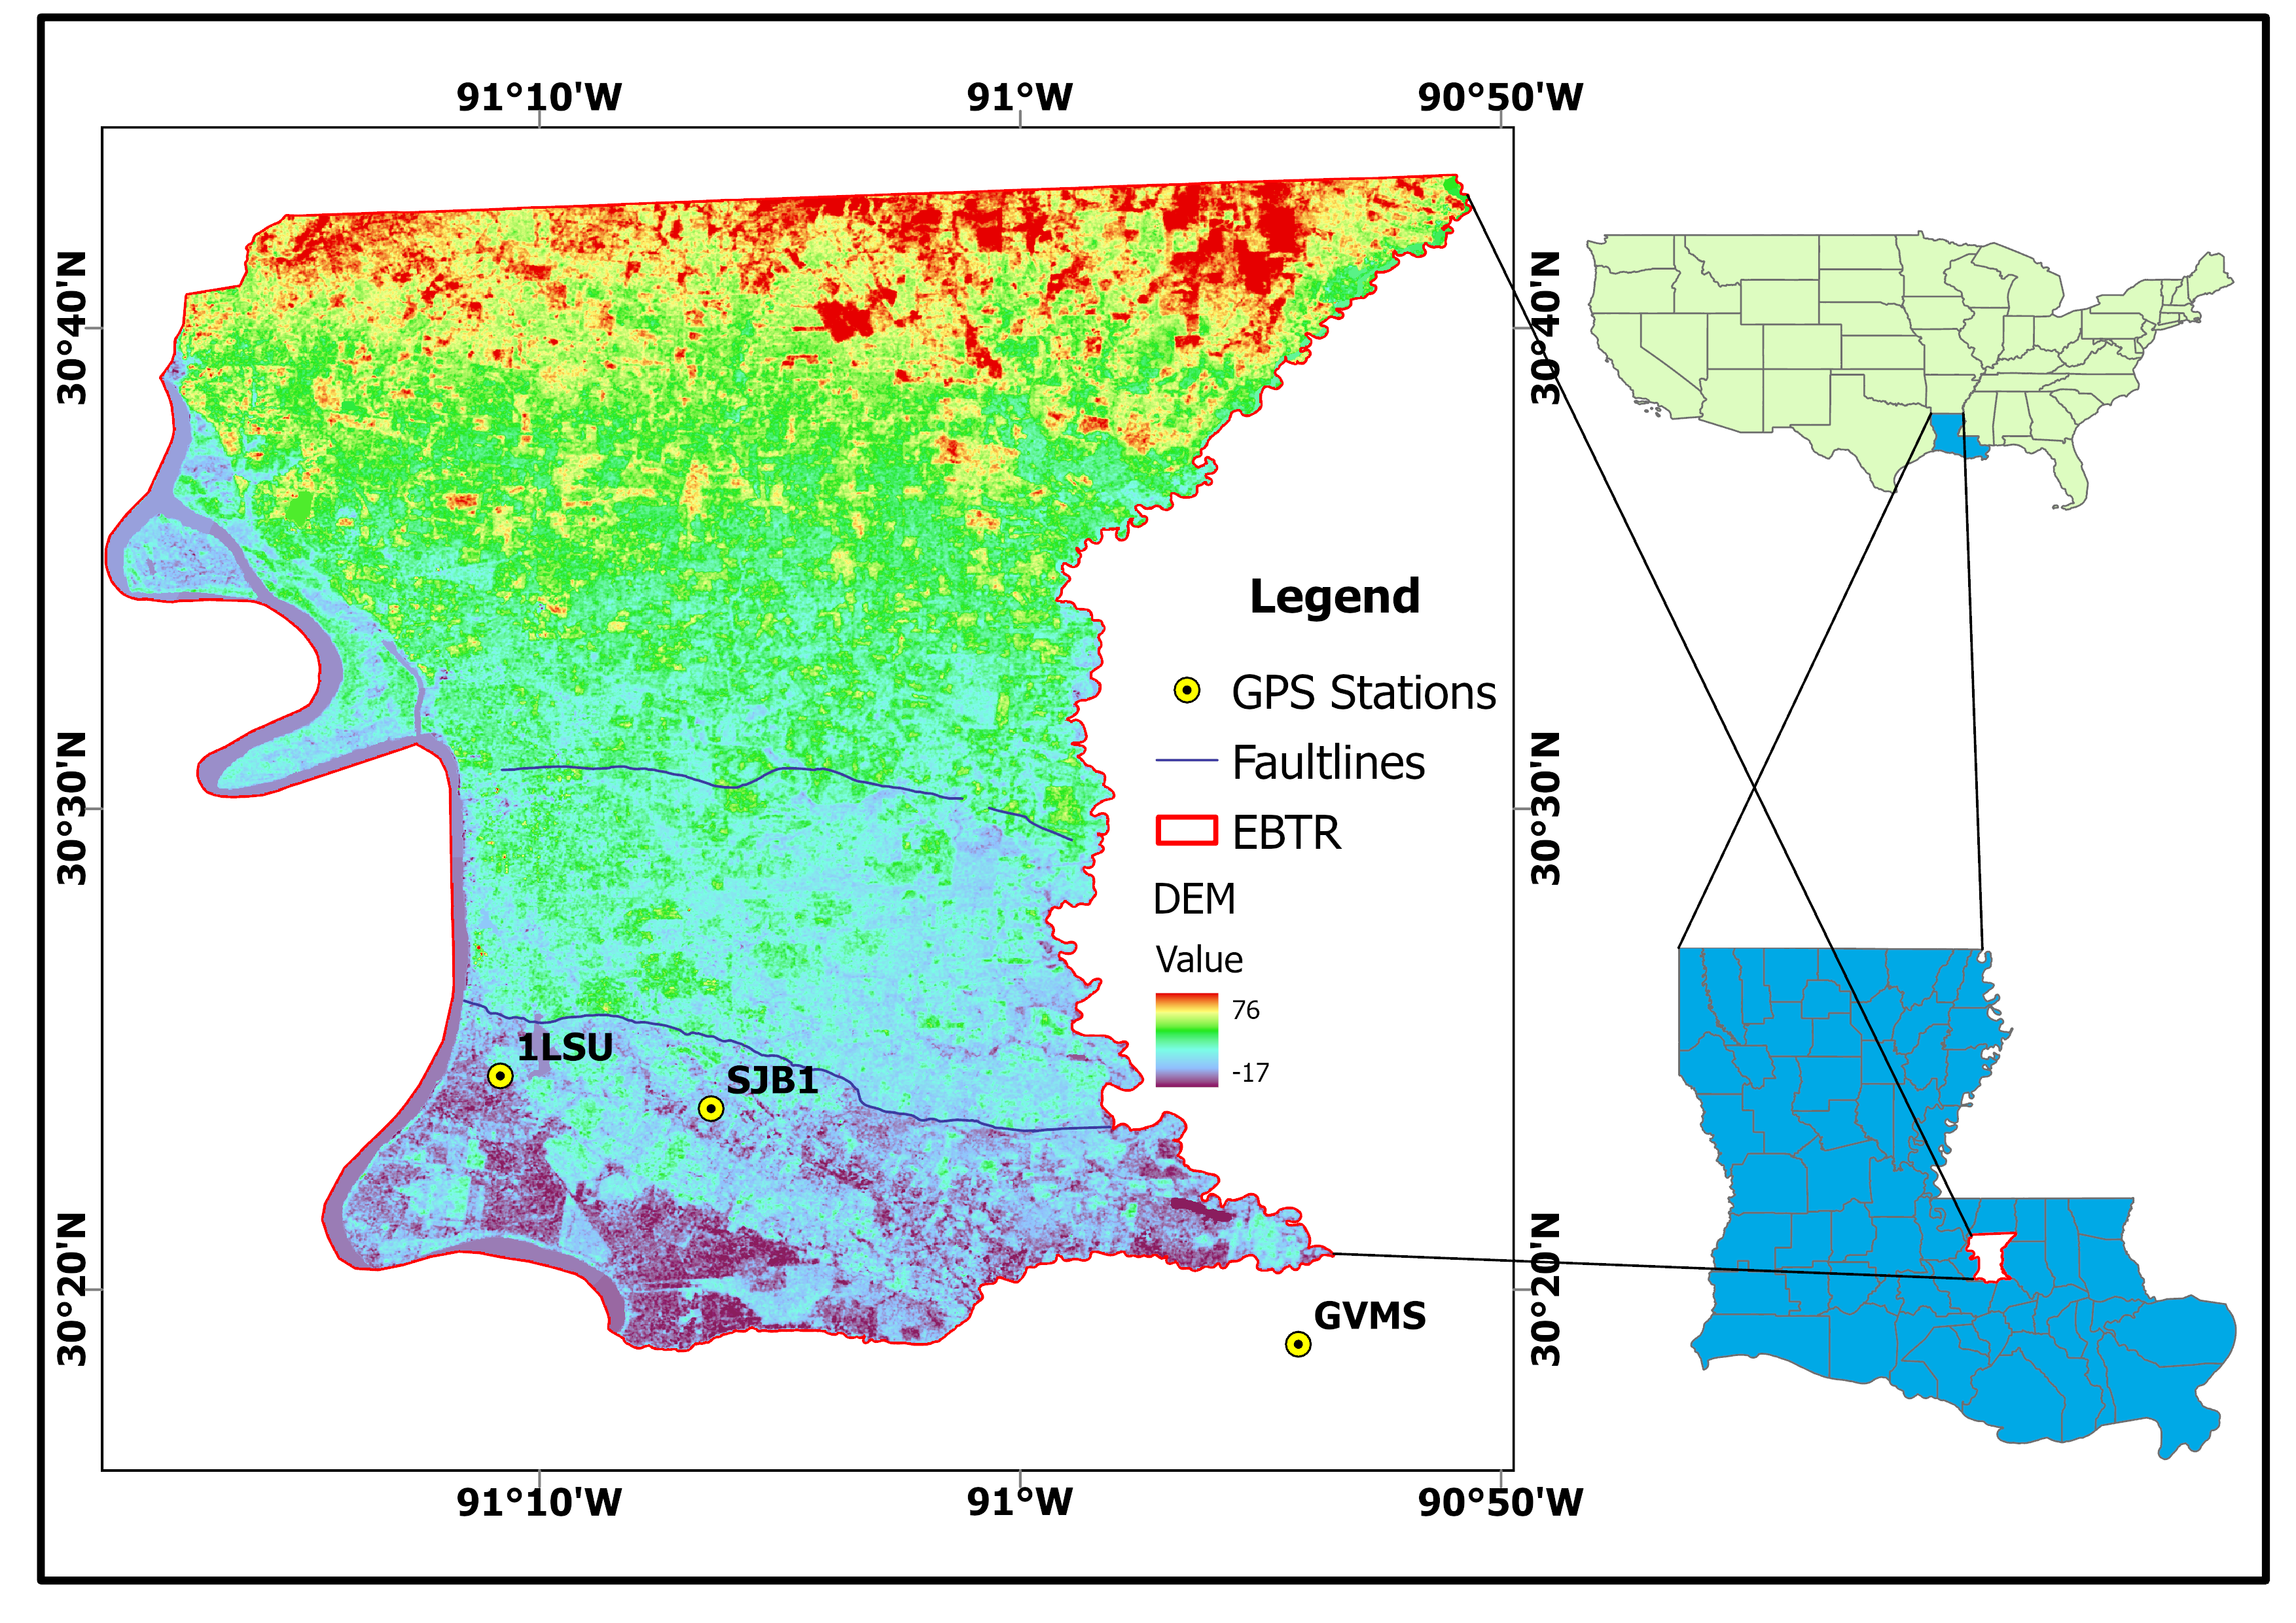
\includegraphics[width=\textwidth,keepaspectratio]{media/AreaLayout.png}
\caption{Location map of East Baton Rouge Parish}
\label{fig:study_area}
\end{figure}

Having established the geophysical and environmental context of EBRP, the following chapter reviews the current state of knowledge in InSAR-based subsidence monitoring, machine learning susceptibility mapping, and temporal forecasting approaches that form the methodological foundation of this study.

\section{Materials}
This study utilises a comprehensive set of satellite data, auxiliary geospatial datasets,
atmospheric products, and open-source software tools to derive eight (8) years (2017-2025) of ground 
deformation and velocity estimates using timeseries SBAS-InSAR techniques.
The materials used are described in detail below.
\subsection{Sentinel-1 SAR Dataset}
The primary SAR dataset consists of 246 Sentinel-1A Single Look Complex (SLC) images acquired in Interferometric Wide (IW) swath mode with VV polarisation. Sentinel-1 is a C-band (5.405 GHz) SAR mission operated by the European Space Agency (ESA) and provides systematic, long-term observations suitable for deformation monitoring. The key acquisition parameters are summarized in Table~\ref{tab:sar_parameters}.

\begin{table}[!t]
\centering
\caption{Main parameters of Sentinel-1A SAR images used in this study}
\label{tab:sar_parameters}
\begin{tabular}{ll}
\hline
\textbf{Parameter} & \textbf{Value} \\
\hline
Product type & Sentinel-1A \\
Data type & SLC \\
Wavelength & C (5.63 cm) \\
Beam mode & IW \\
Revisit period & 12 days \\
Polarization & VV \\
Start time & January 2017 \\
End time & July 2025 \\
Path & 63 \\
Frame & 92 \\
Orbit direction & Ascending \\
Incidence angle & 39.6$^\circ$ \\
Resolution & 5m$\times$20m \\
\hline
\end{tabular}
\end{table}

The Sentinel-1 frame (Path 63, Frame 92) covers a broad geographic extent across southeastern Louisiana, with corner coordinates at 30$^\circ$17$'$52.54$''$N, 93$^\circ$20$'$30.29$''$W (northwest), 30$^\circ$43$'$10.97$''$N, 90$^\circ$43$'$51.95$''$W (northeast), 29$^\circ$5$'$39.31$''$N, 90$^\circ$23$'$52.42$''$W (southeast), and 28$^\circ$40$'$51.69$''$N, 92$^\circ$57$'$3.61$''$W (southwest). East Baton Rouge Parish constitutes a small subset within this larger frame, and the SBAS-InSAR processing was applied to the full frame extent before extracting the study area domain. This approach ensures consistent atmospheric correction and phase unwrapping across regional scales while enabling focused analysis of EBRP.

\subsection{Precise Orbit Ephemerides}
Precise Orbits Ephemerides (POEORB) provided by the ESA were applied to all Sentinel-1 acquisitions
prior to interferometric processing. Compared to restituted orbits, POEORB significantly improves 
satellite position accuracy, reducing residual orbital errors and mitigating long-wavelength phase ramps
in interferograms \citep{Ferretti2001}.

\subsection{Digital Elevation Model and Atmospheric Data}
A 30 m resolution Digital Elevation Model (DEM) was used to correct for topographic phase contributions 
in interferograms generation. The DEM also served as the basis for deriving topographic conditioning factors
used in the susceptibility analysis. 

To mitigate atmospheric artefacts, particularly stratified tropospheric delays, ERA5
(Fifth Generation ECMWF Atmospheric Reanalysis) data were incorporated during timeseries 
processing. ERA5 provides high-resolution global estimates of atmospheric state variables and has been 
widely adopted for atmospheric phase screen correction in InSAR studies \citep{HosseinzadehLLand2024}.

\subsection{Geospatial Conditioning Factors}
A total of fifteen (15) geospatial conditioning factors were prepared at 30 m resolution and 
aligned to a common spatial grid for land subsidence susceptibility modelling.
These factors were grouped into topographic, geological, hydrological, structural/tectonic, infrastructure, climatic, and anthropogenic categories, reflecting the multi-causal nature of land subsidence processes (Figures~\ref{fig:topo_factors}--\ref{fig:anthro_factors}).

\subsubsection{Topographic Factors}
Six topographic attributes were derived from the 30 m DEM: elevation, slope, aspect, Topographic Position Index (TPI), curvature, and Topographic Wetness Index (TWI). These parameters characterize terrain morphology and control surface water flow, soil moisture distribution, and differential loading conditions that influence subsidence susceptibility.

\begin{figure}[htbp]
\centering
\begin{tabular}{cc}
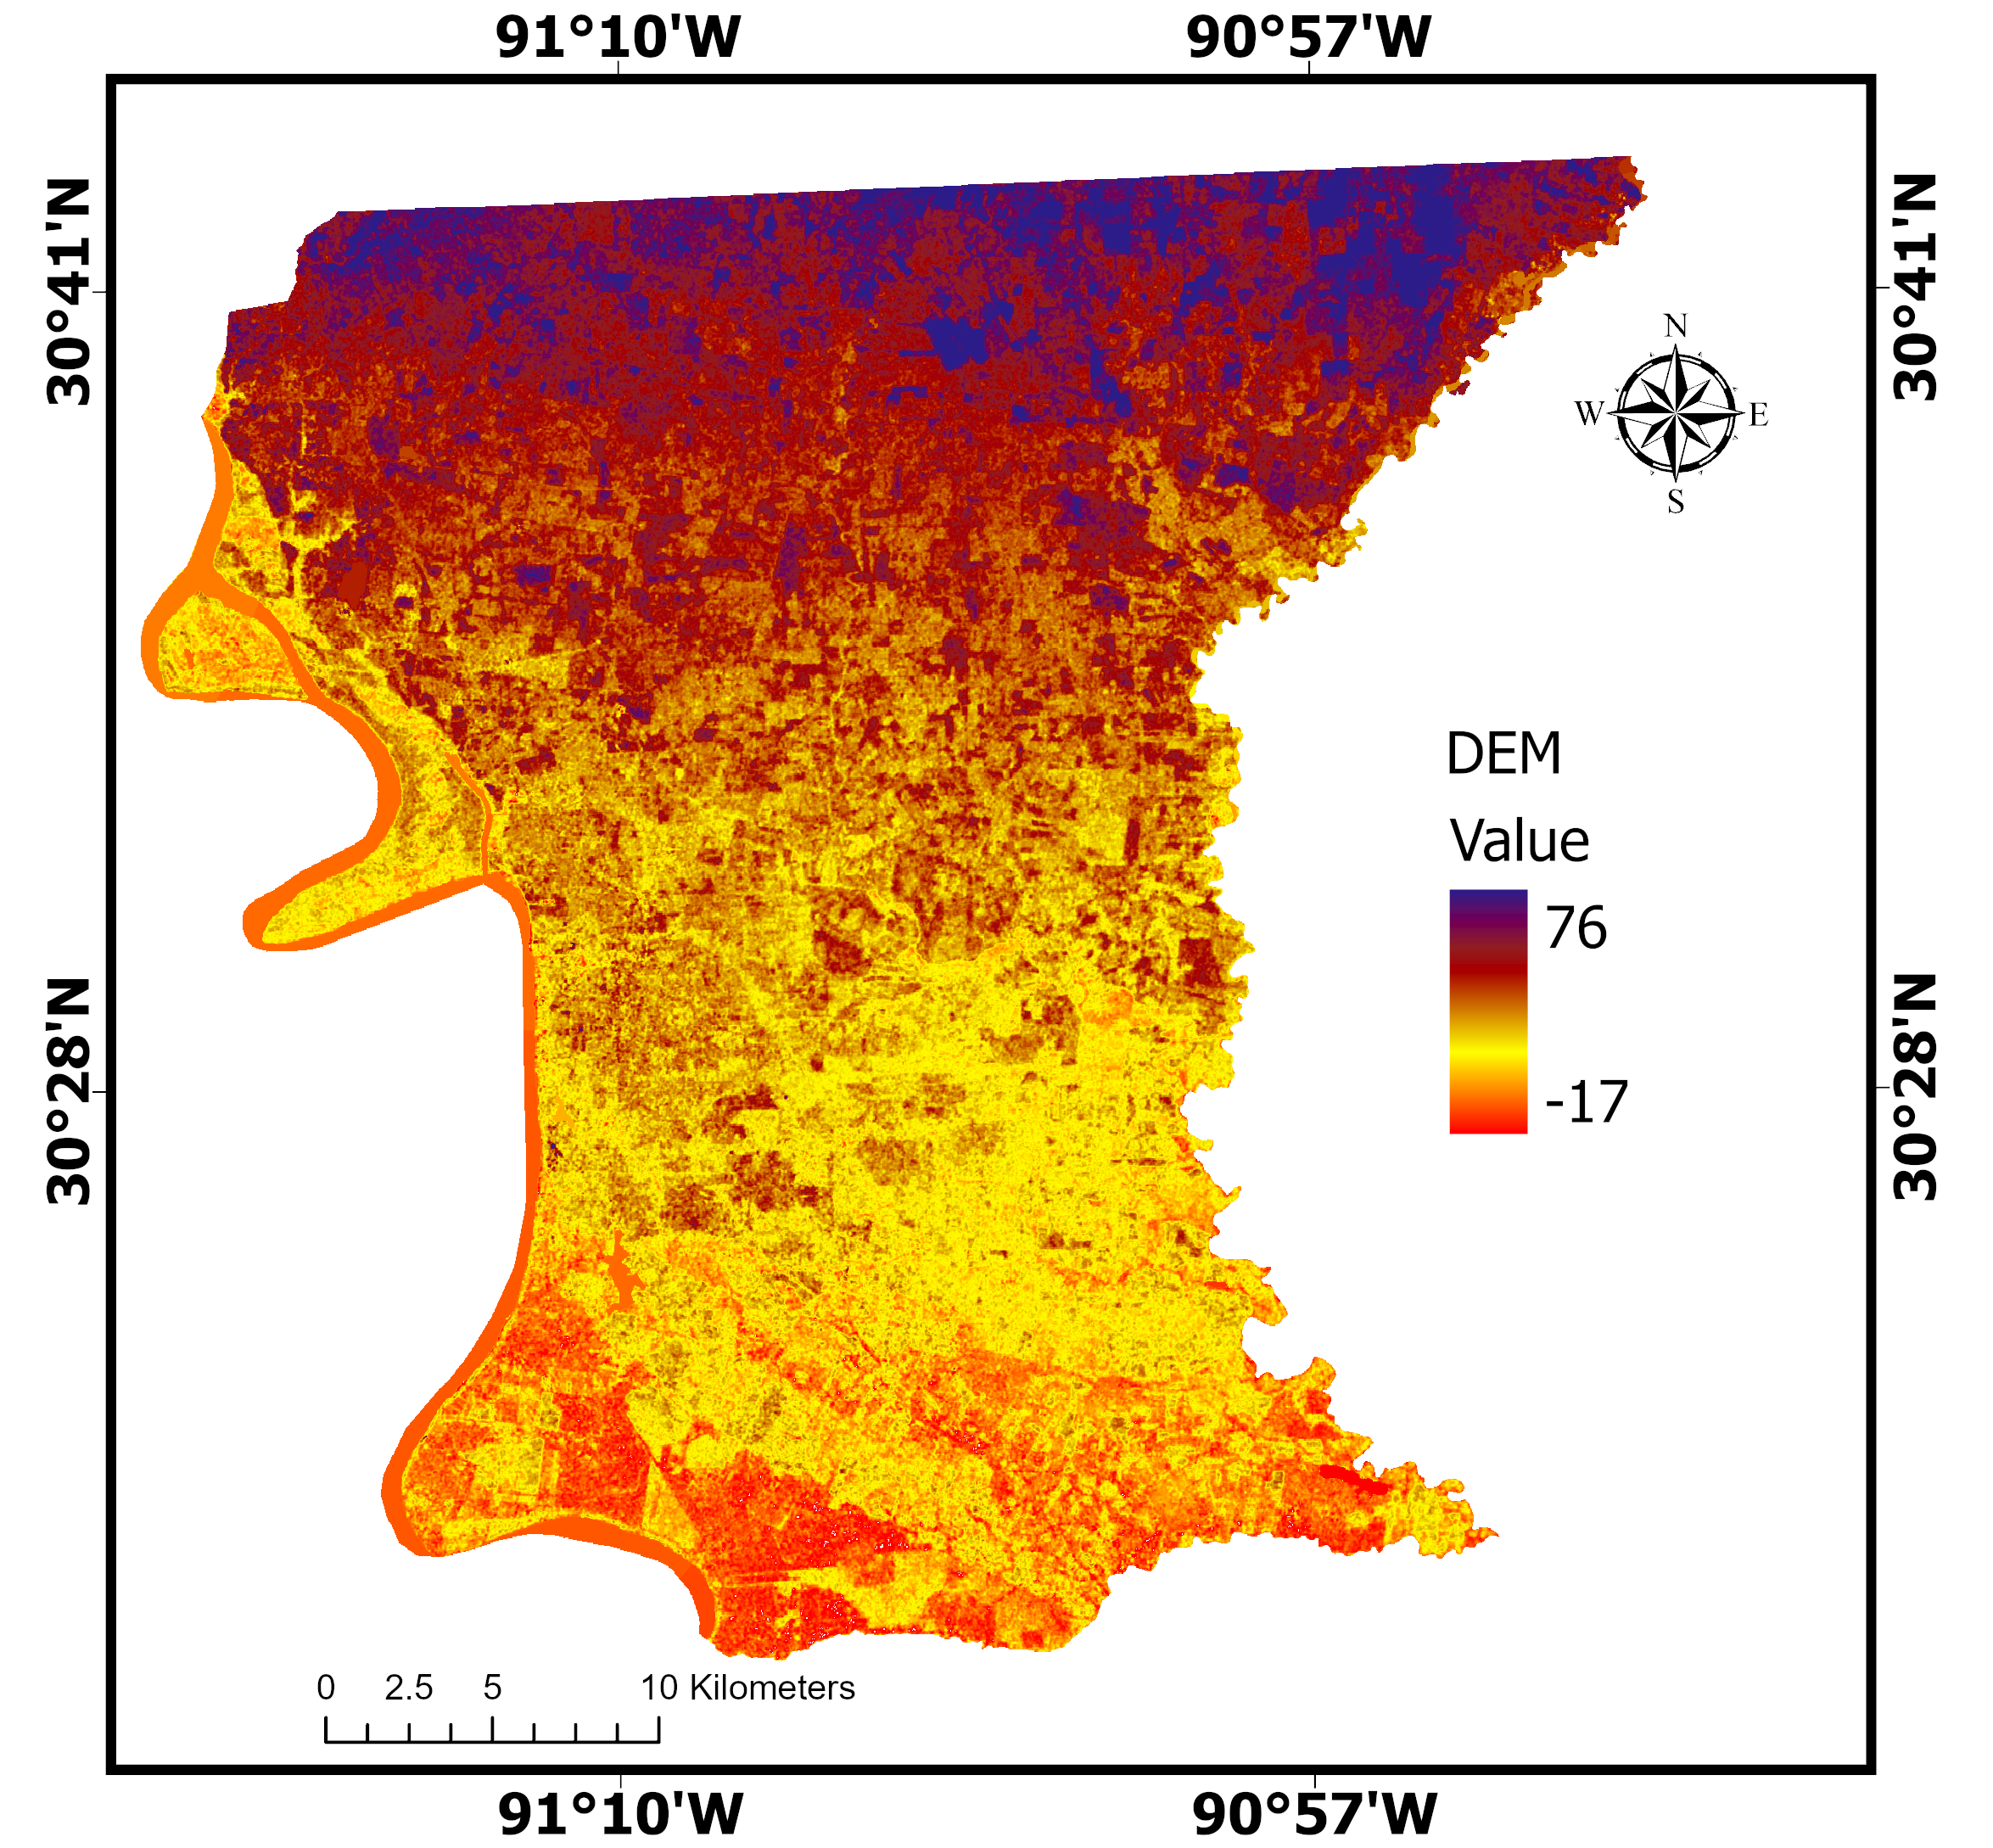
\includegraphics[width=0.48\textwidth]{All_layers/dem.png} &
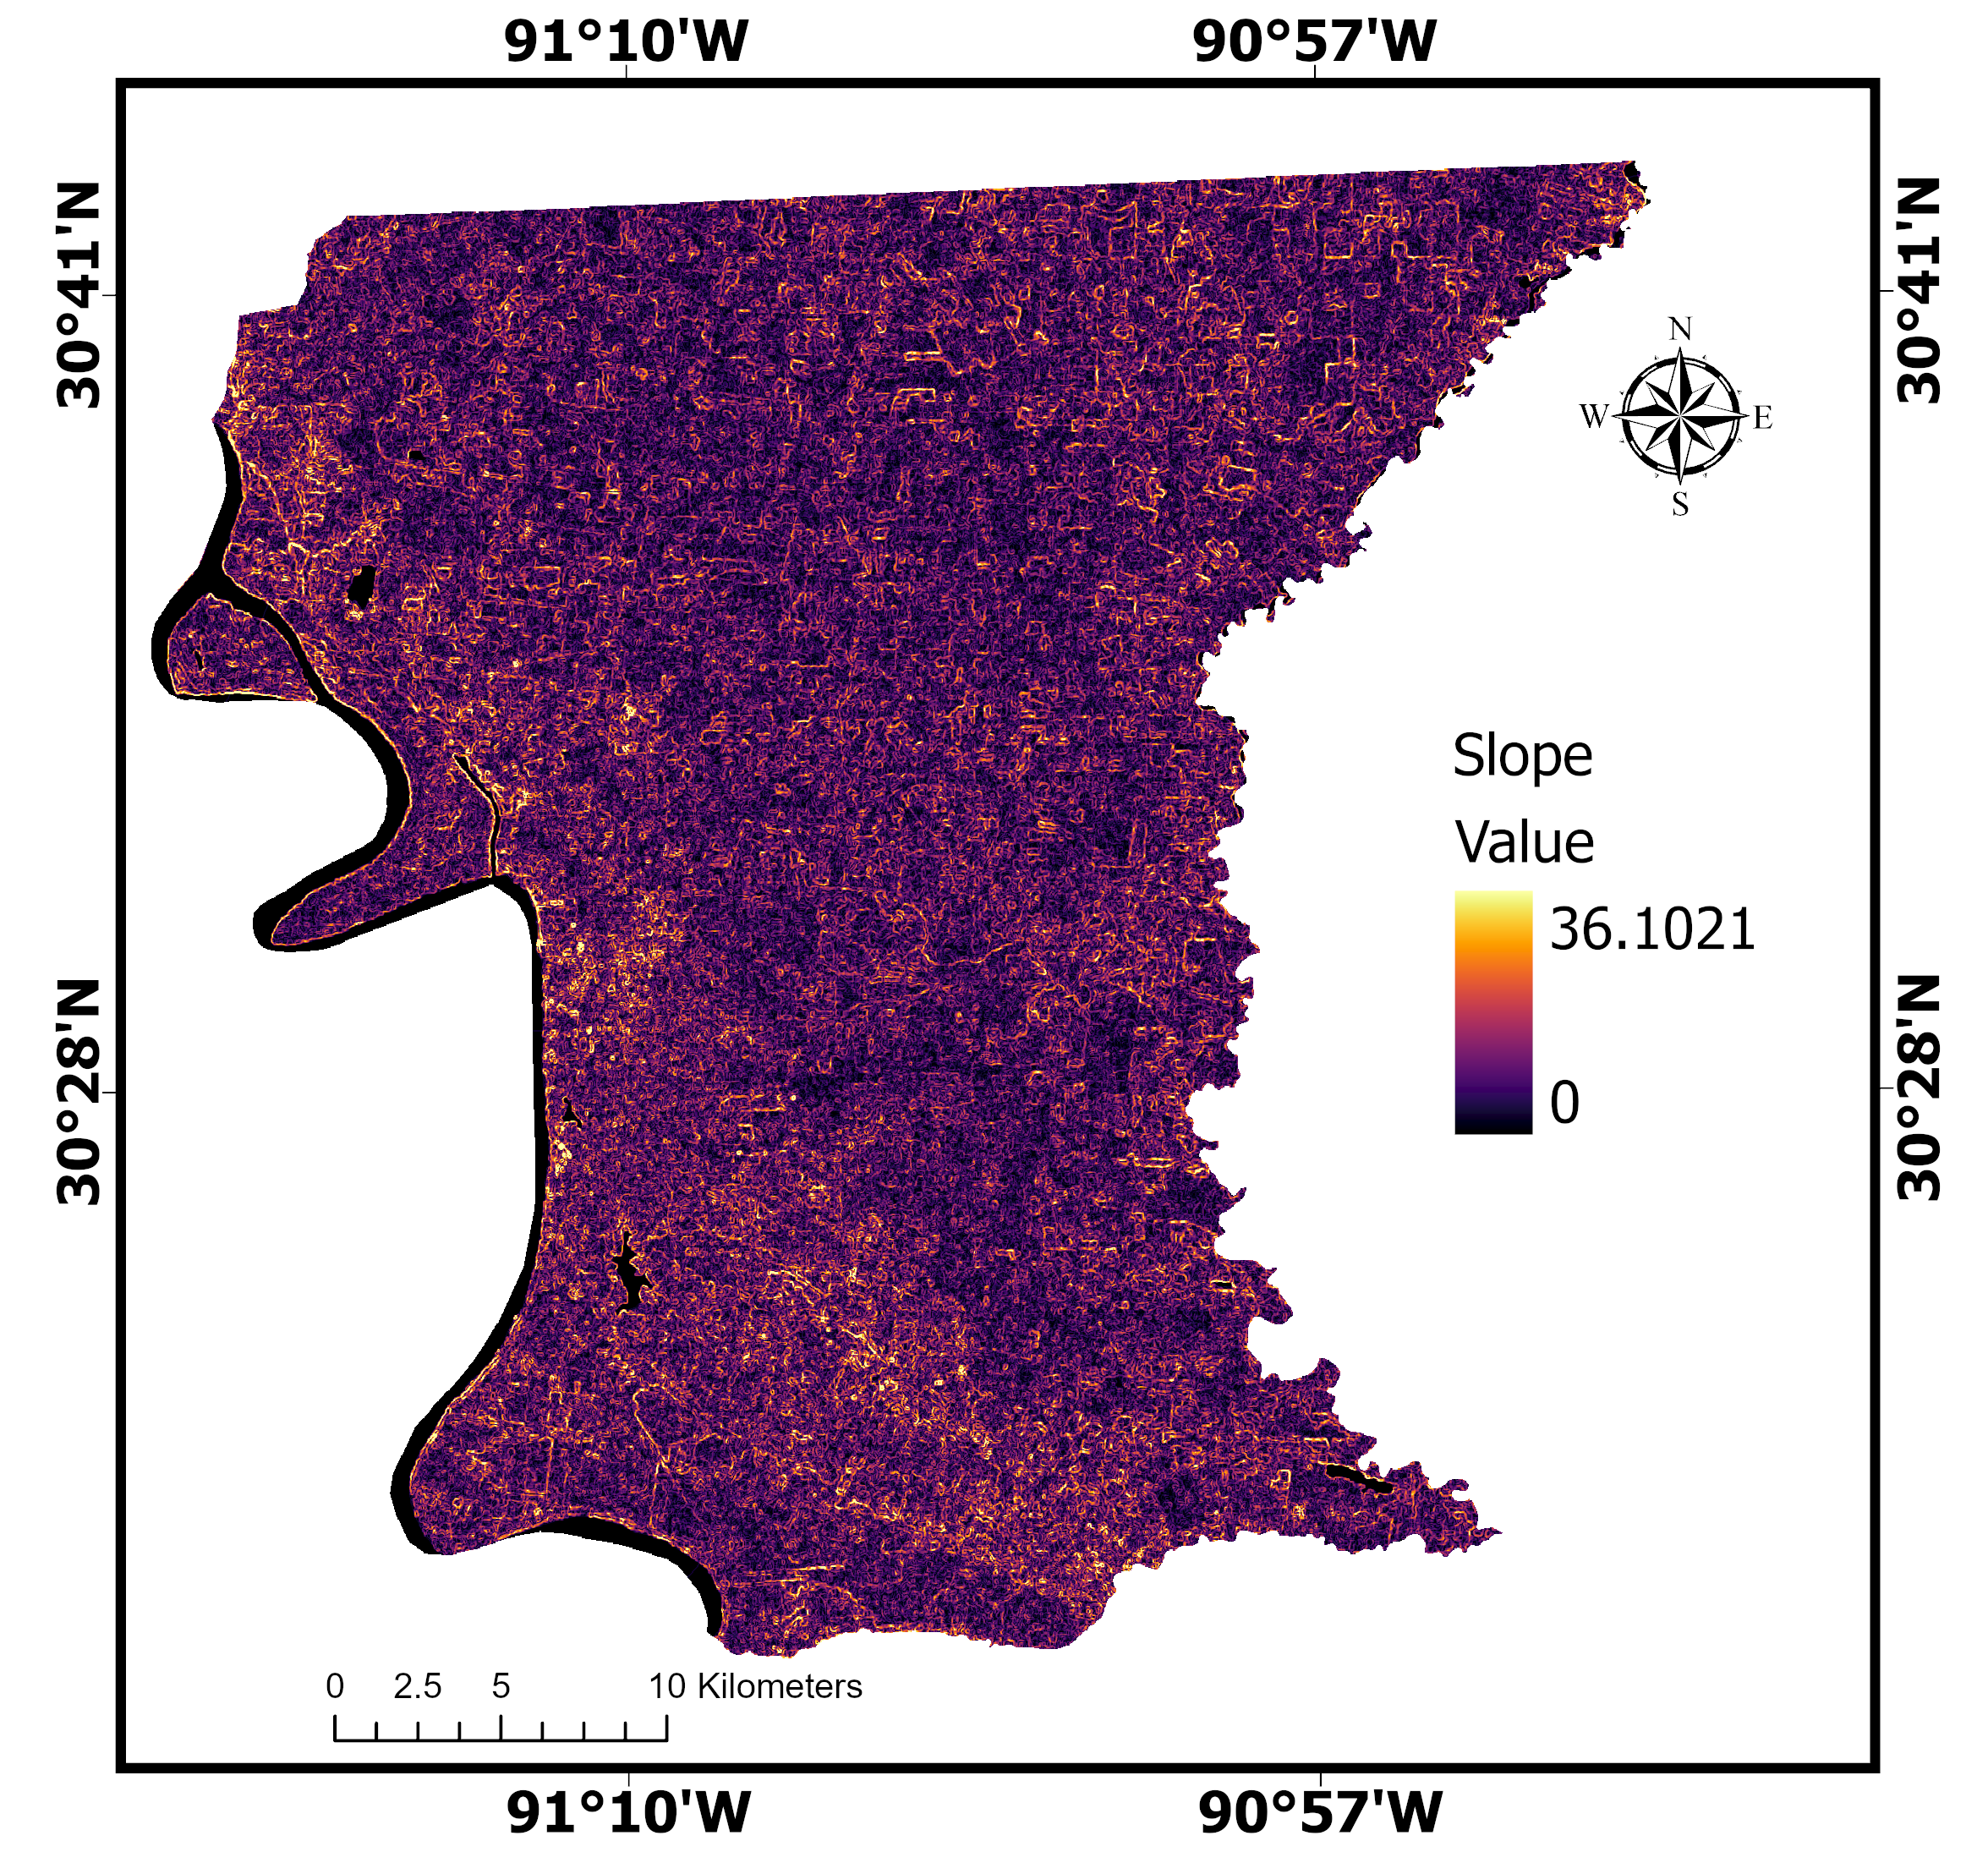
\includegraphics[width=0.48\textwidth]{All_layers/slope.png} \\
(a) Digital Elevation Model & (b) Slope \\
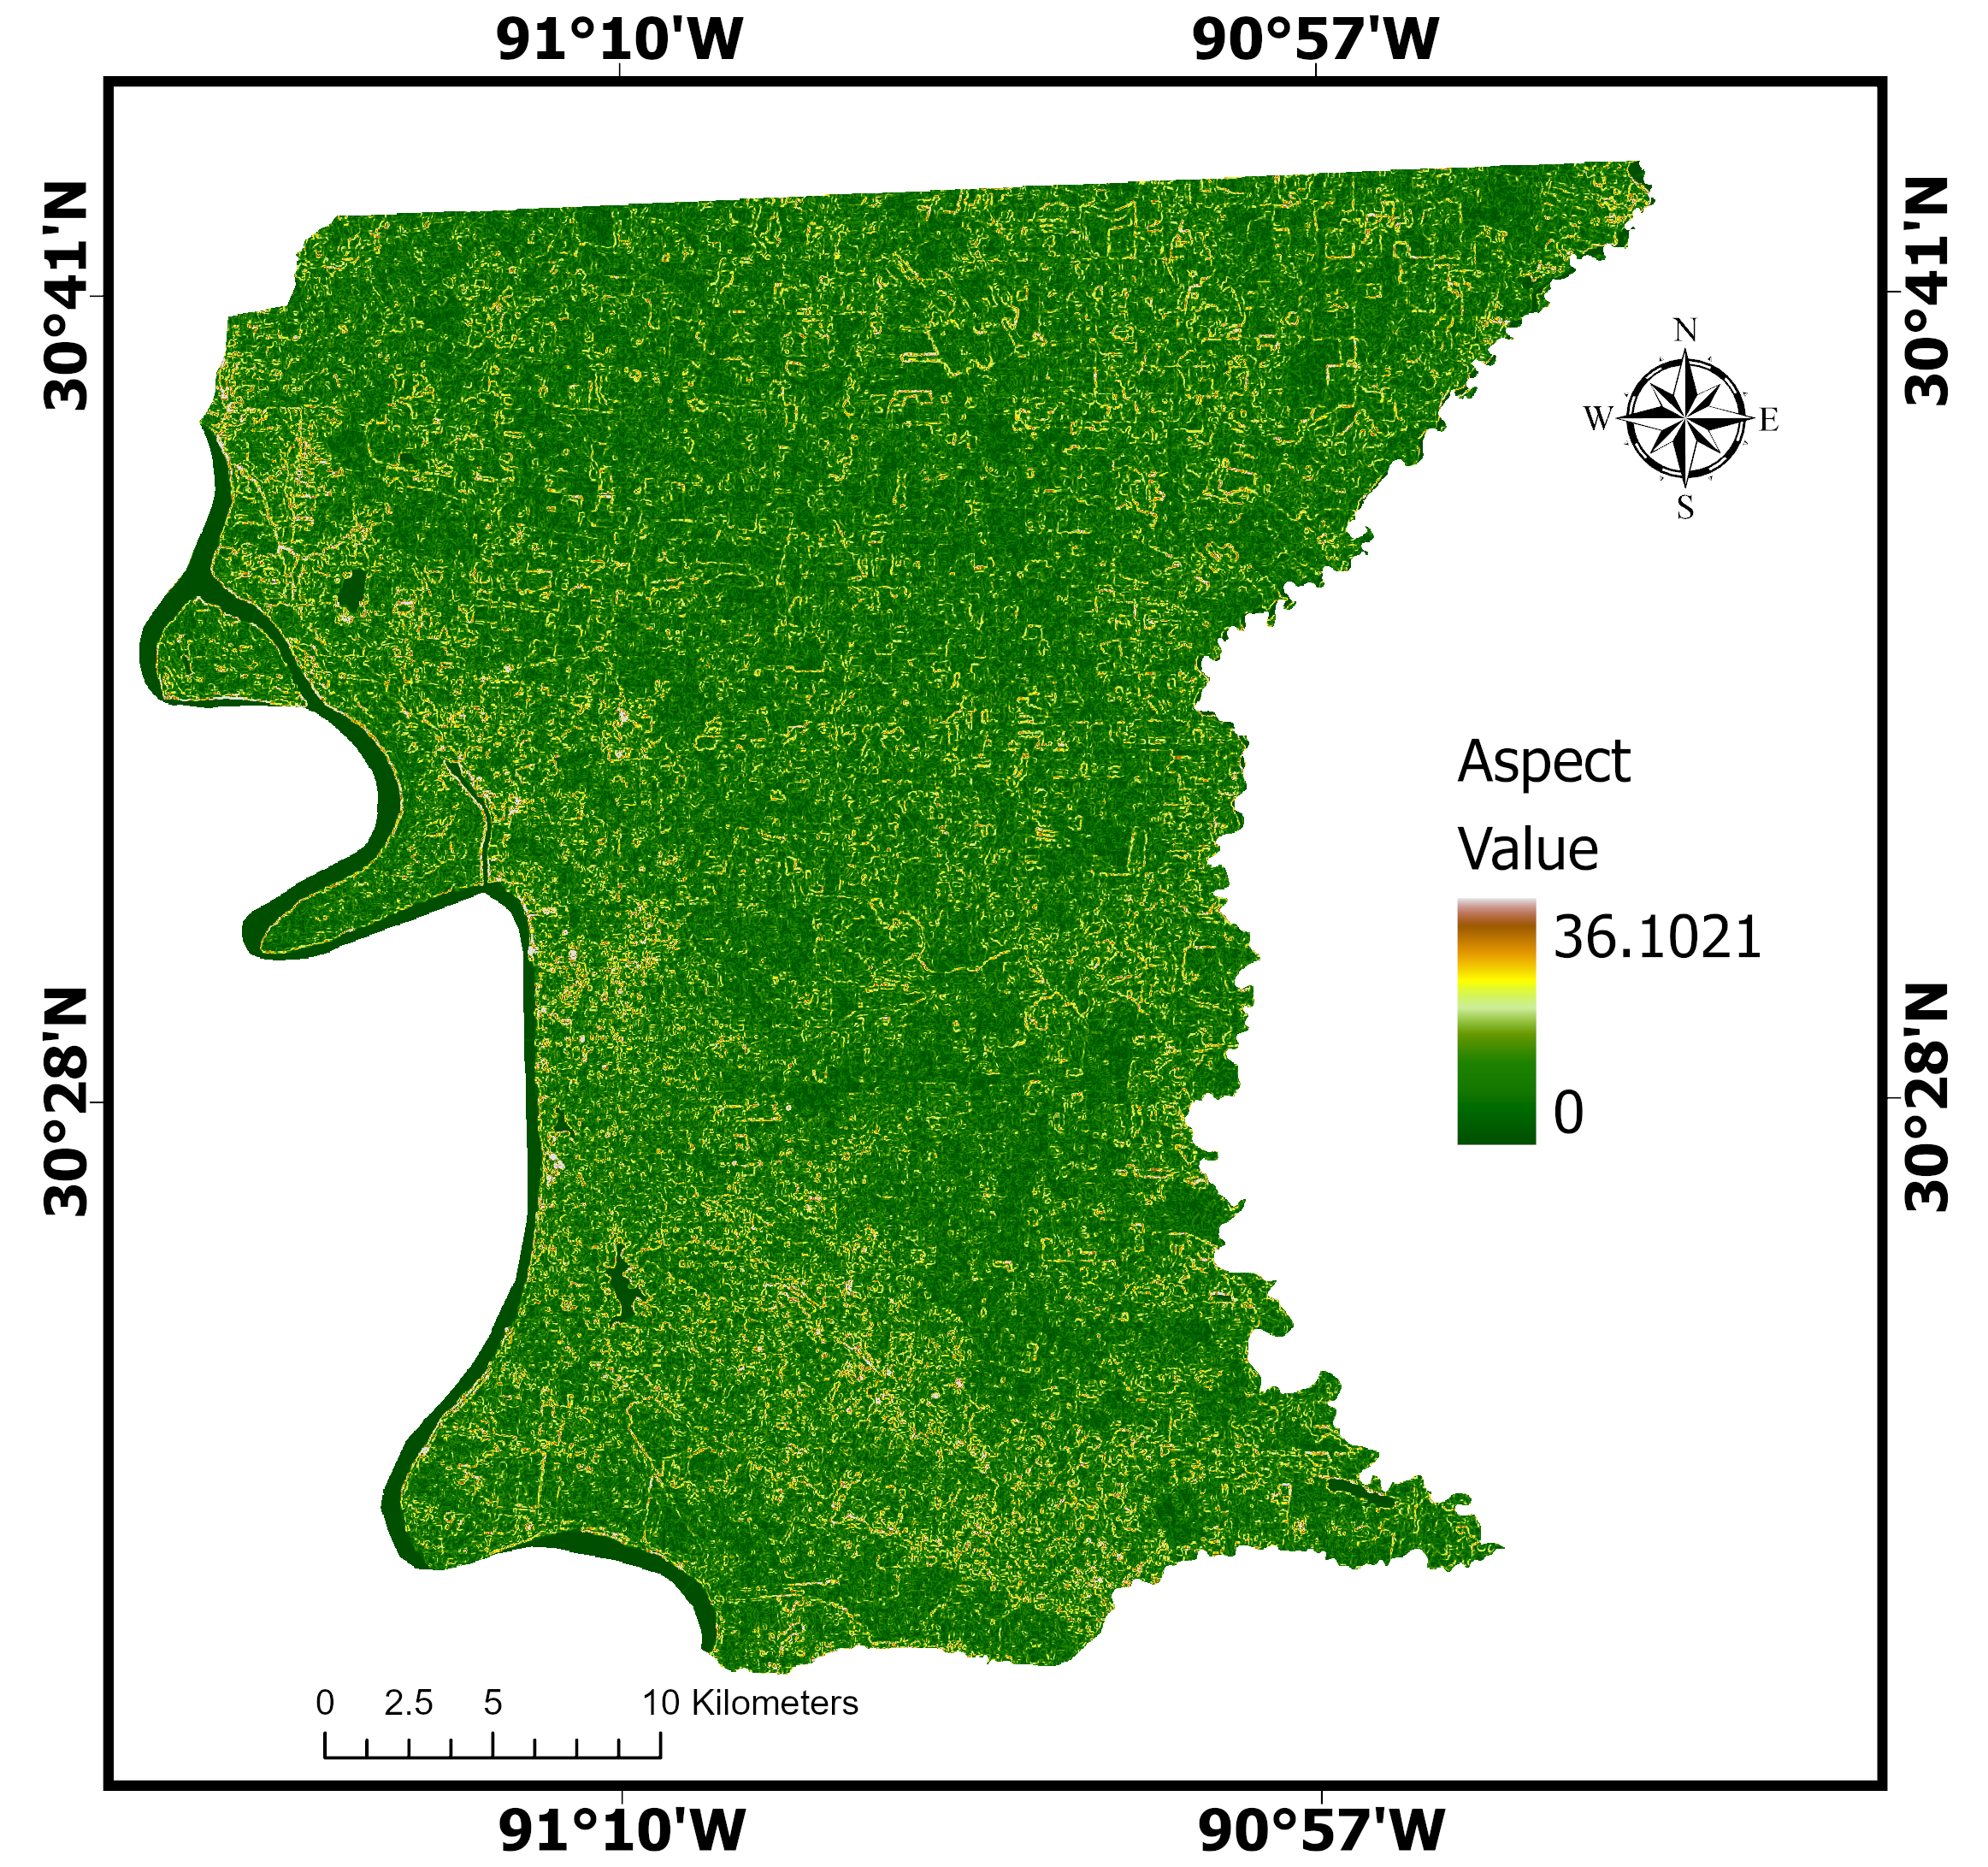
\includegraphics[width=0.48\textwidth]{All_layers/aspect.png} &
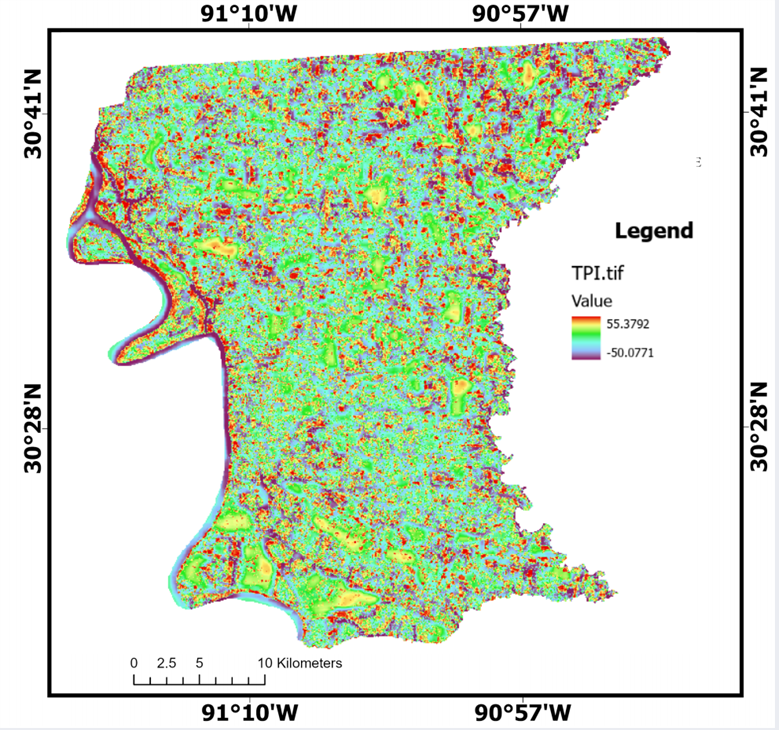
\includegraphics[width=0.48\textwidth]{All_layers/TPI.png} \\
(c) Aspect & (d) Topographic Position Index \\
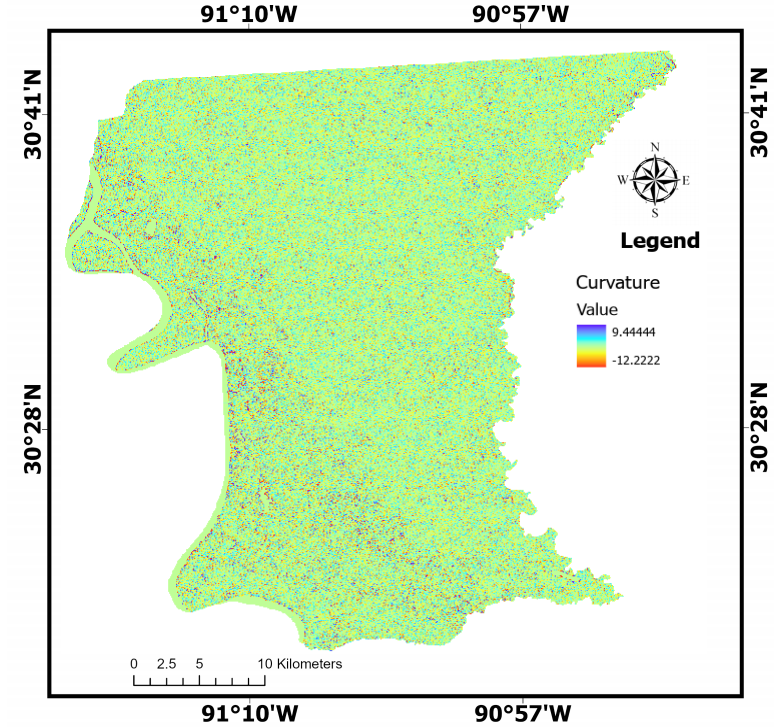
\includegraphics[width=0.48\textwidth]{All_layers/Curvature.png} &
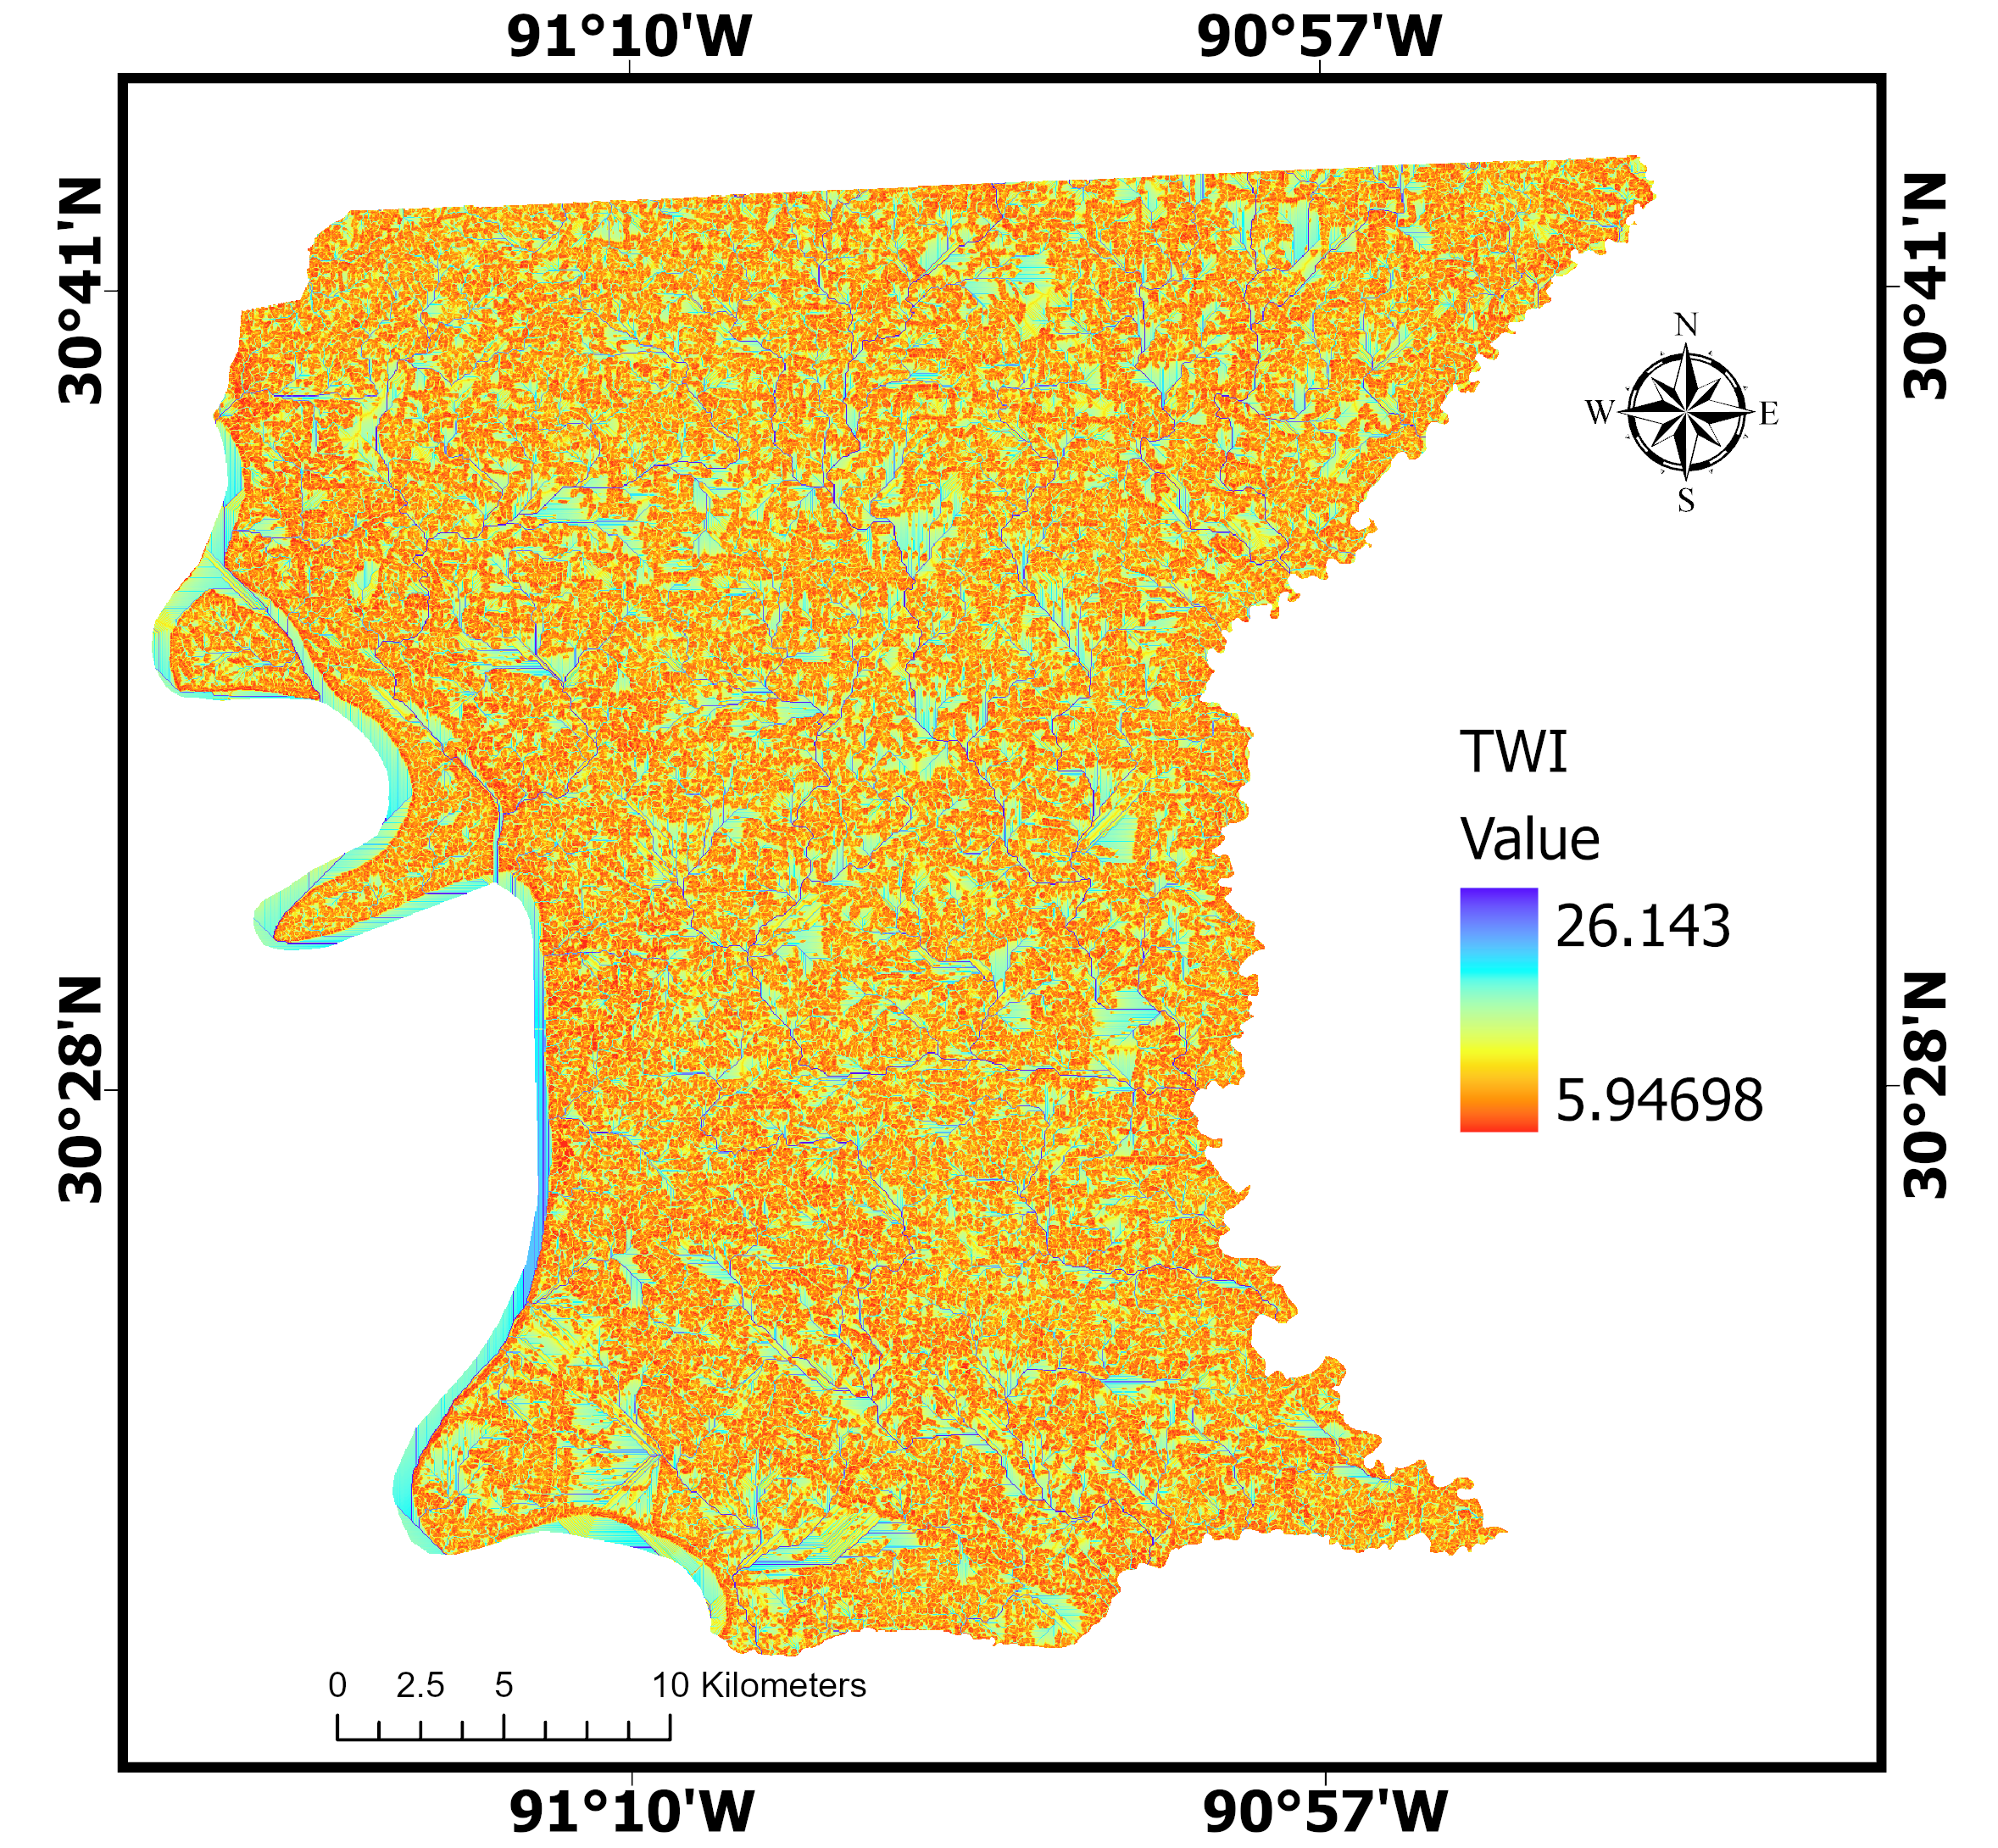
\includegraphics[width=0.48\textwidth]{All_layers/twi.png} \\
(e) Curvature & (f) Topographic Wetness Index
\end{tabular}
\caption{Topographic conditioning factors for subsidence susceptibility mapping}
\label{fig:topo_factors}
\end{figure}

\subsubsection{Geological Factors}
Geological characteristics include bedrock geology and Land Use/Land Cover (LULC), which control subsurface compressibility and surface loading patterns (Figure~\ref{fig:geo_factors}).

\begin{figure}[htbp]
\centering
\begin{tabular}{cc}
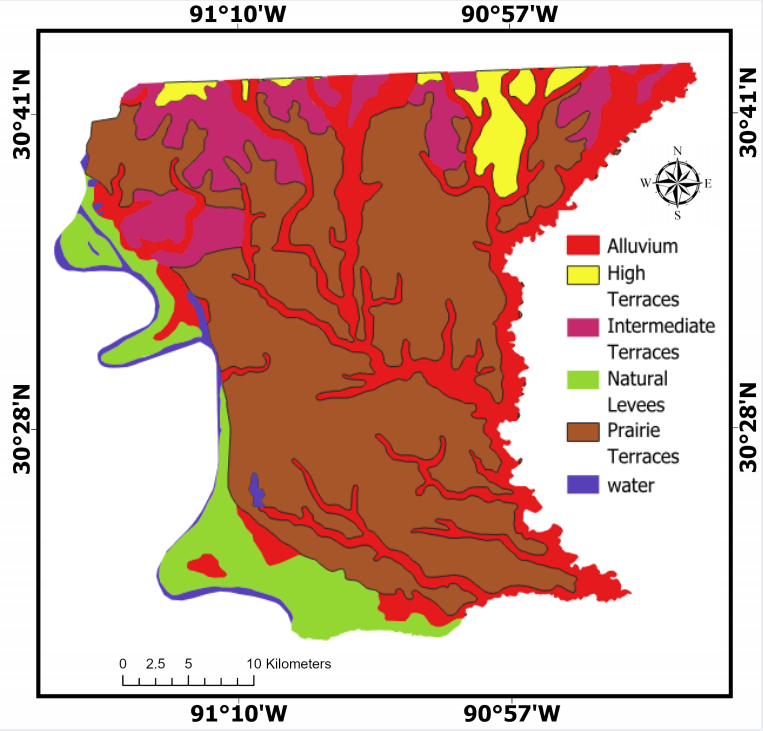
\includegraphics[width=0.48\textwidth]{All_layers/geology.png} &
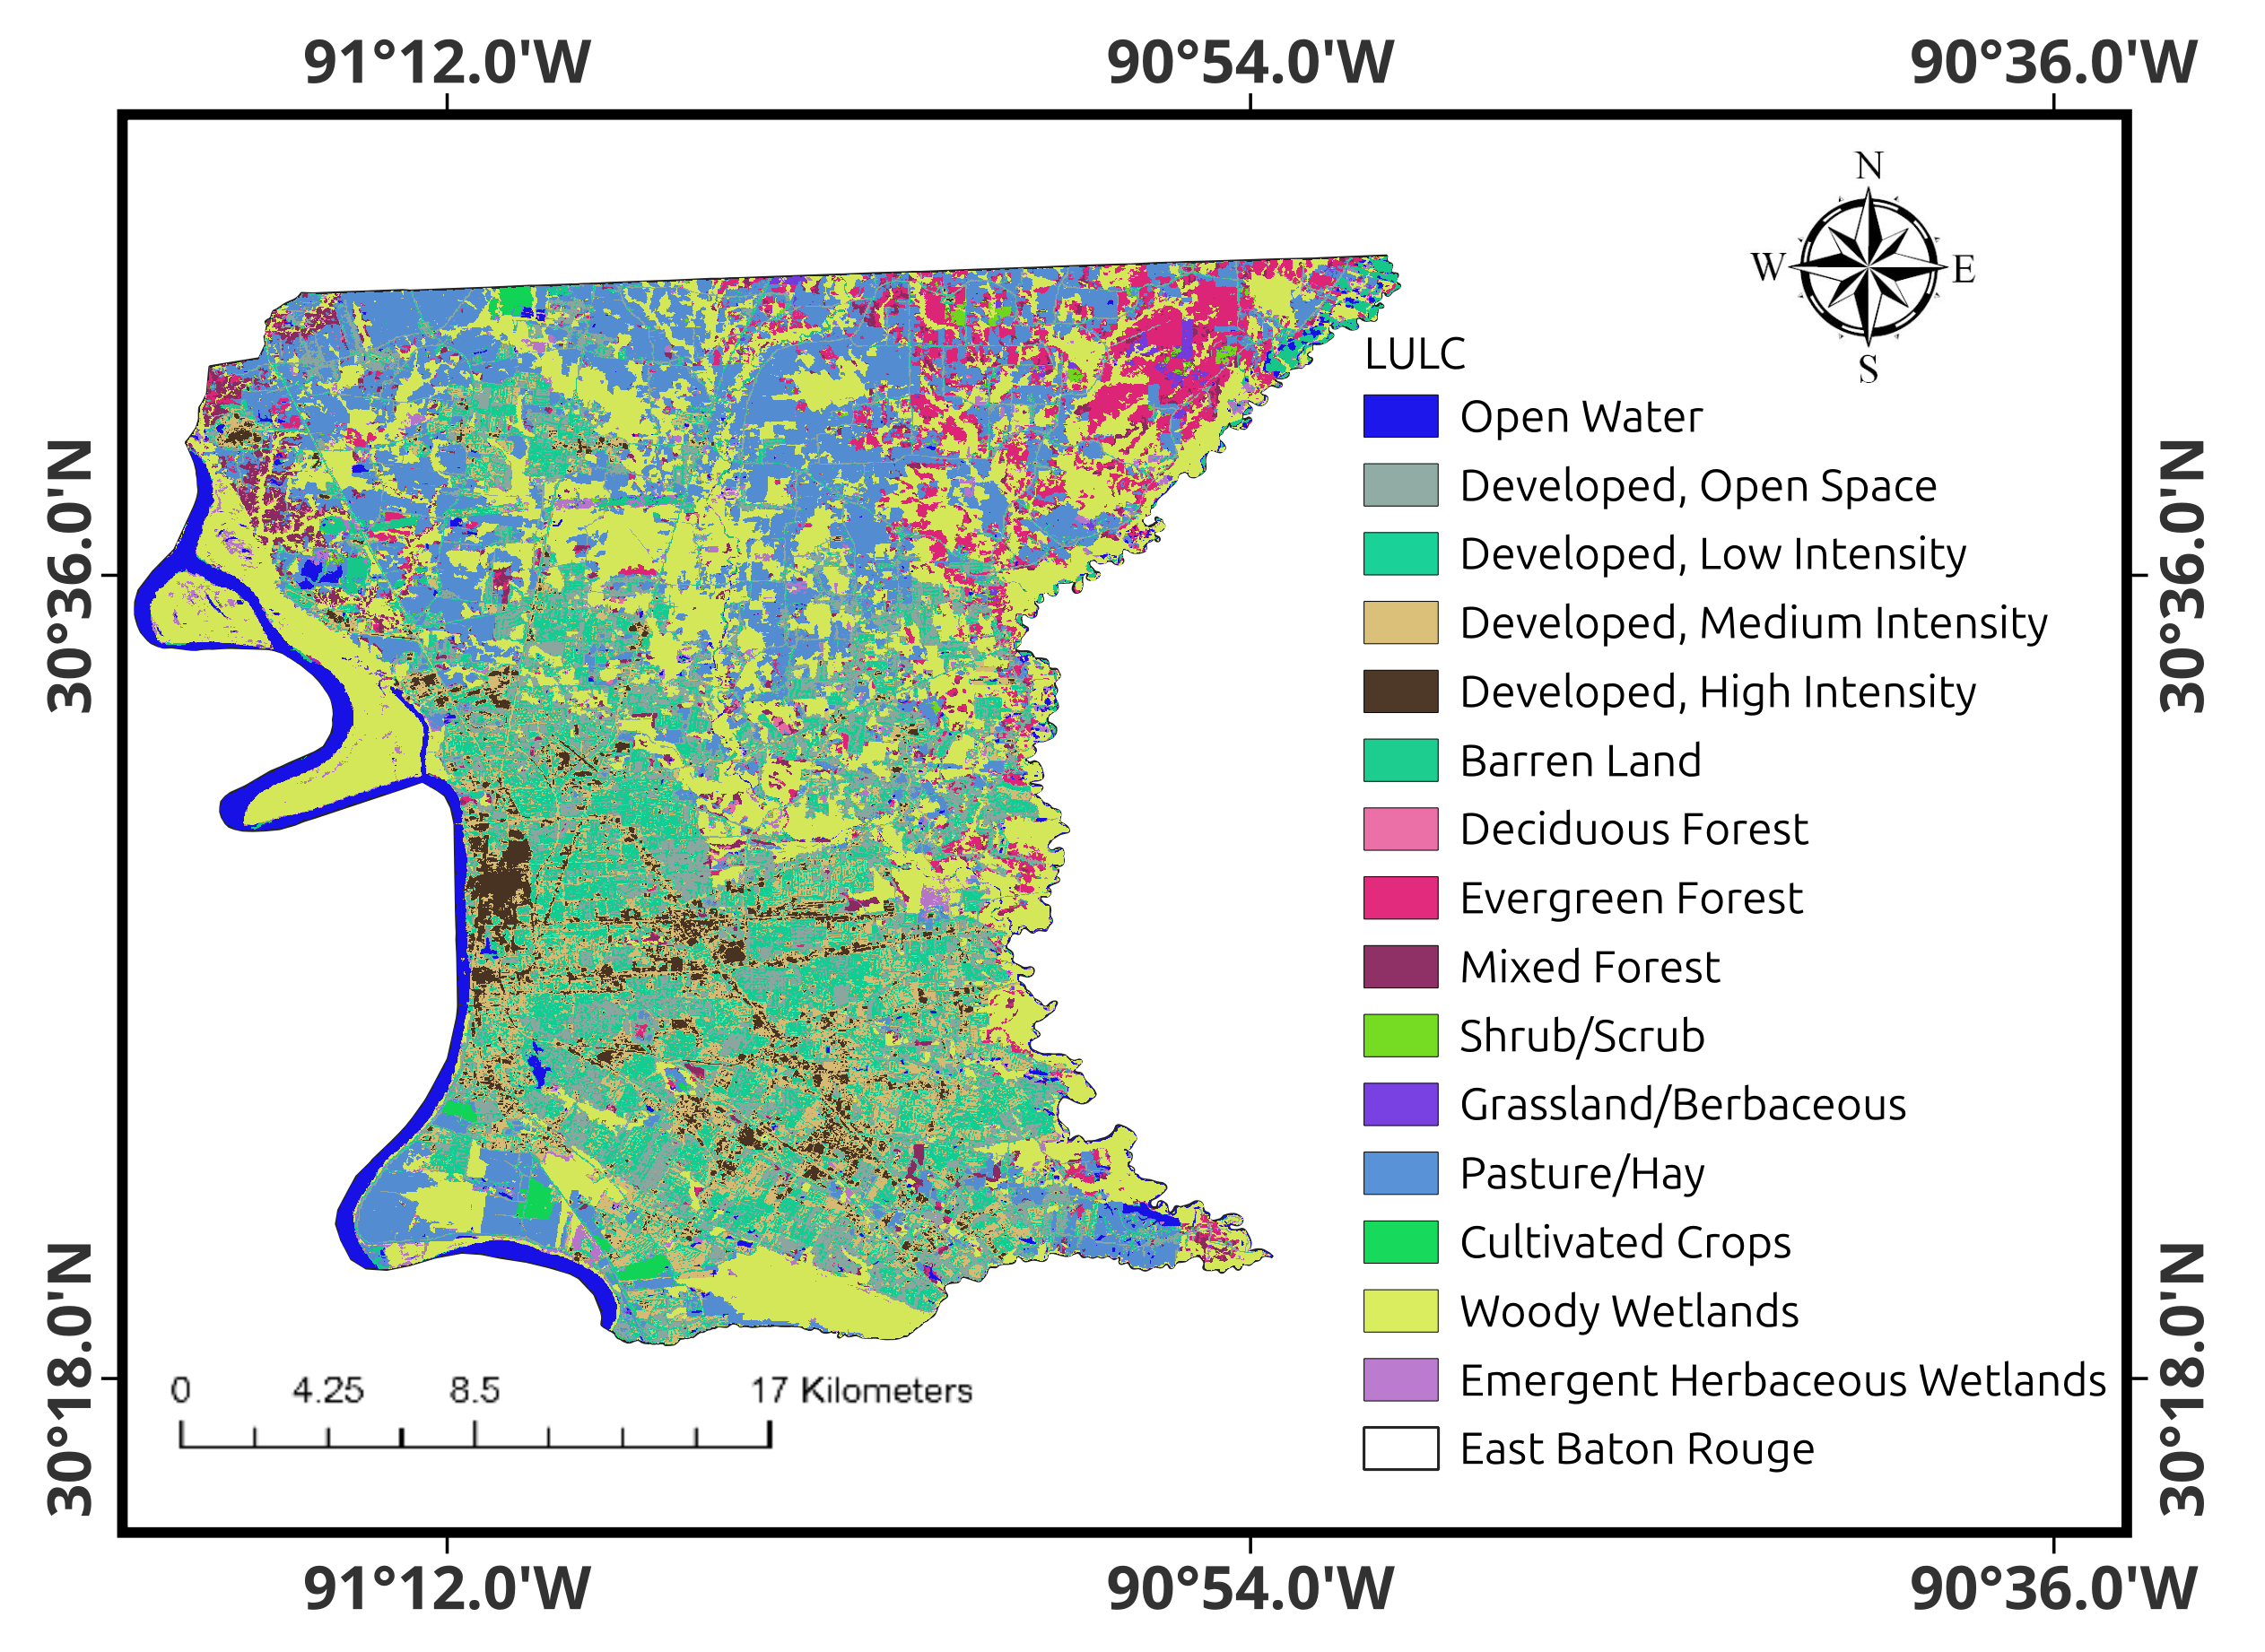
\includegraphics[width=0.48\textwidth]{All_layers/lulcnew.png} \\
(a) Geology & (b) Land Use/Land Cover
\end{tabular}
\caption{Geological conditioning factors}
\label{fig:geo_factors}
\end{figure}

\subsubsection{Hydrological and Structural Factors}
Distance from rivers and faults represent hydrological connectivity and structural controls on subsidence (Figure~\ref{fig:hydro_struct_factors}). The Baton Rouge and Denham Springs fault systems introduce spatially heterogeneous deformation patterns.

\begin{figure}[htbp]
\centering
\begin{tabular}{cc}
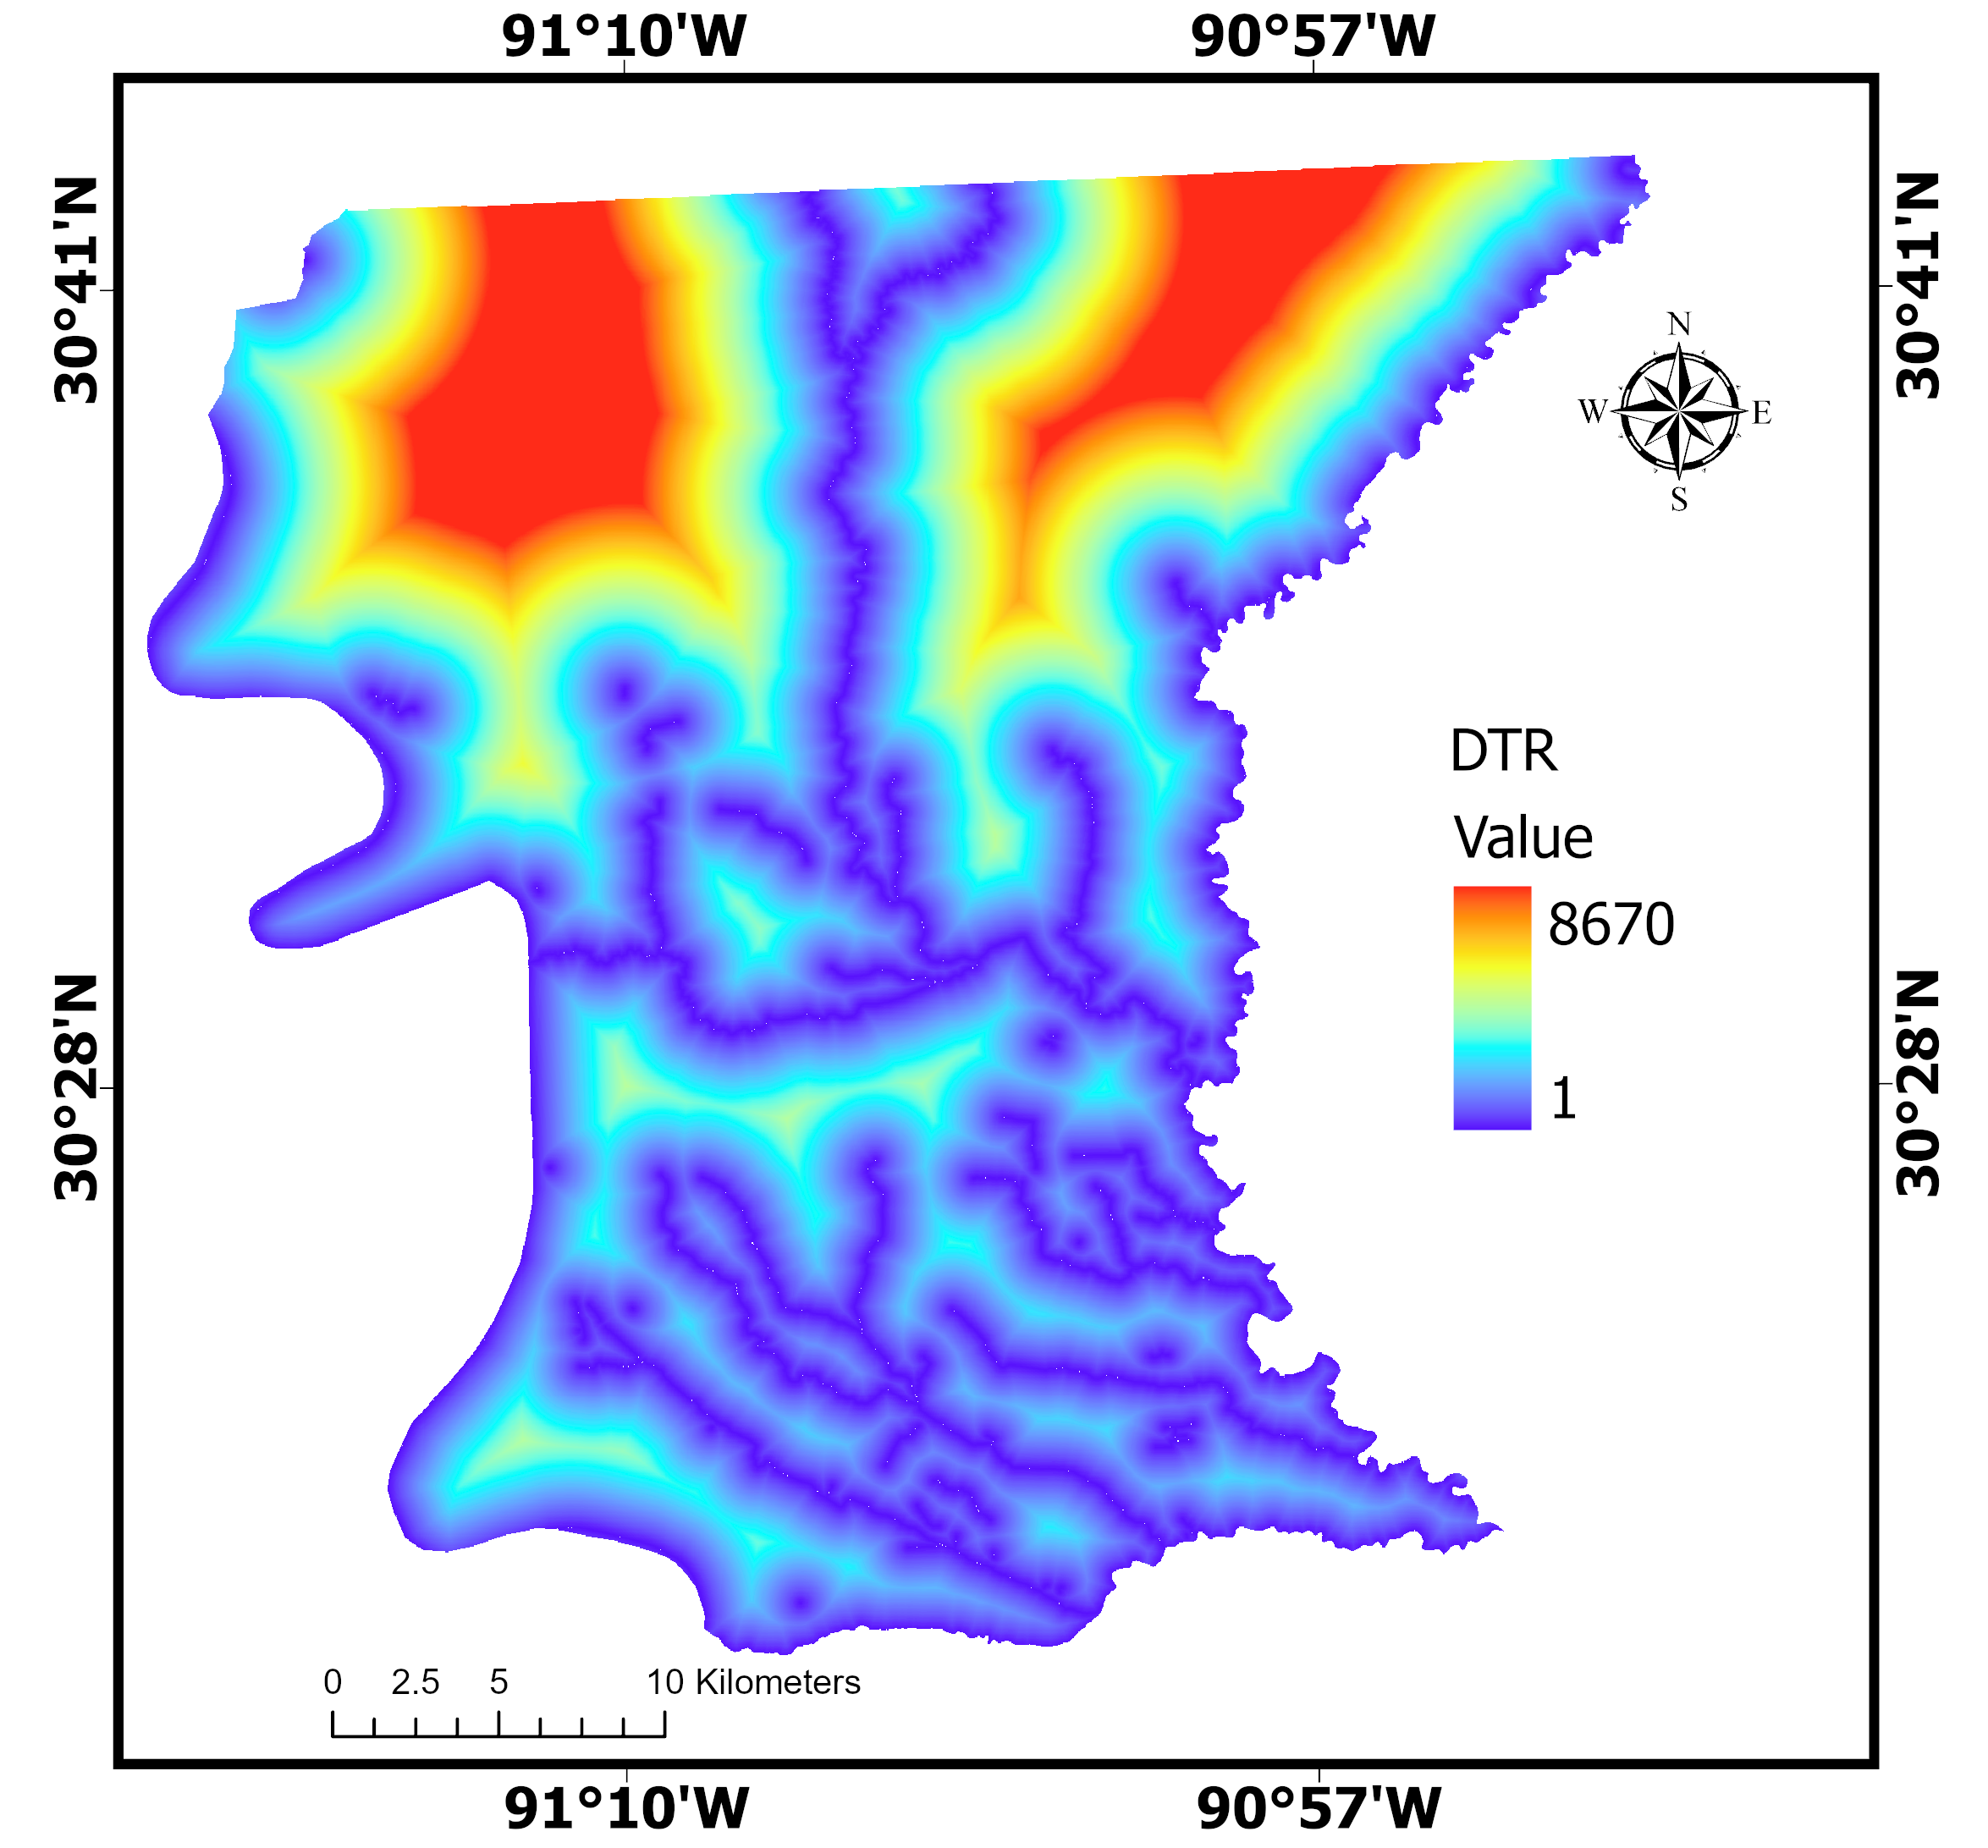
\includegraphics[width=0.48\textwidth]{All_layers/distanceriver.png} &
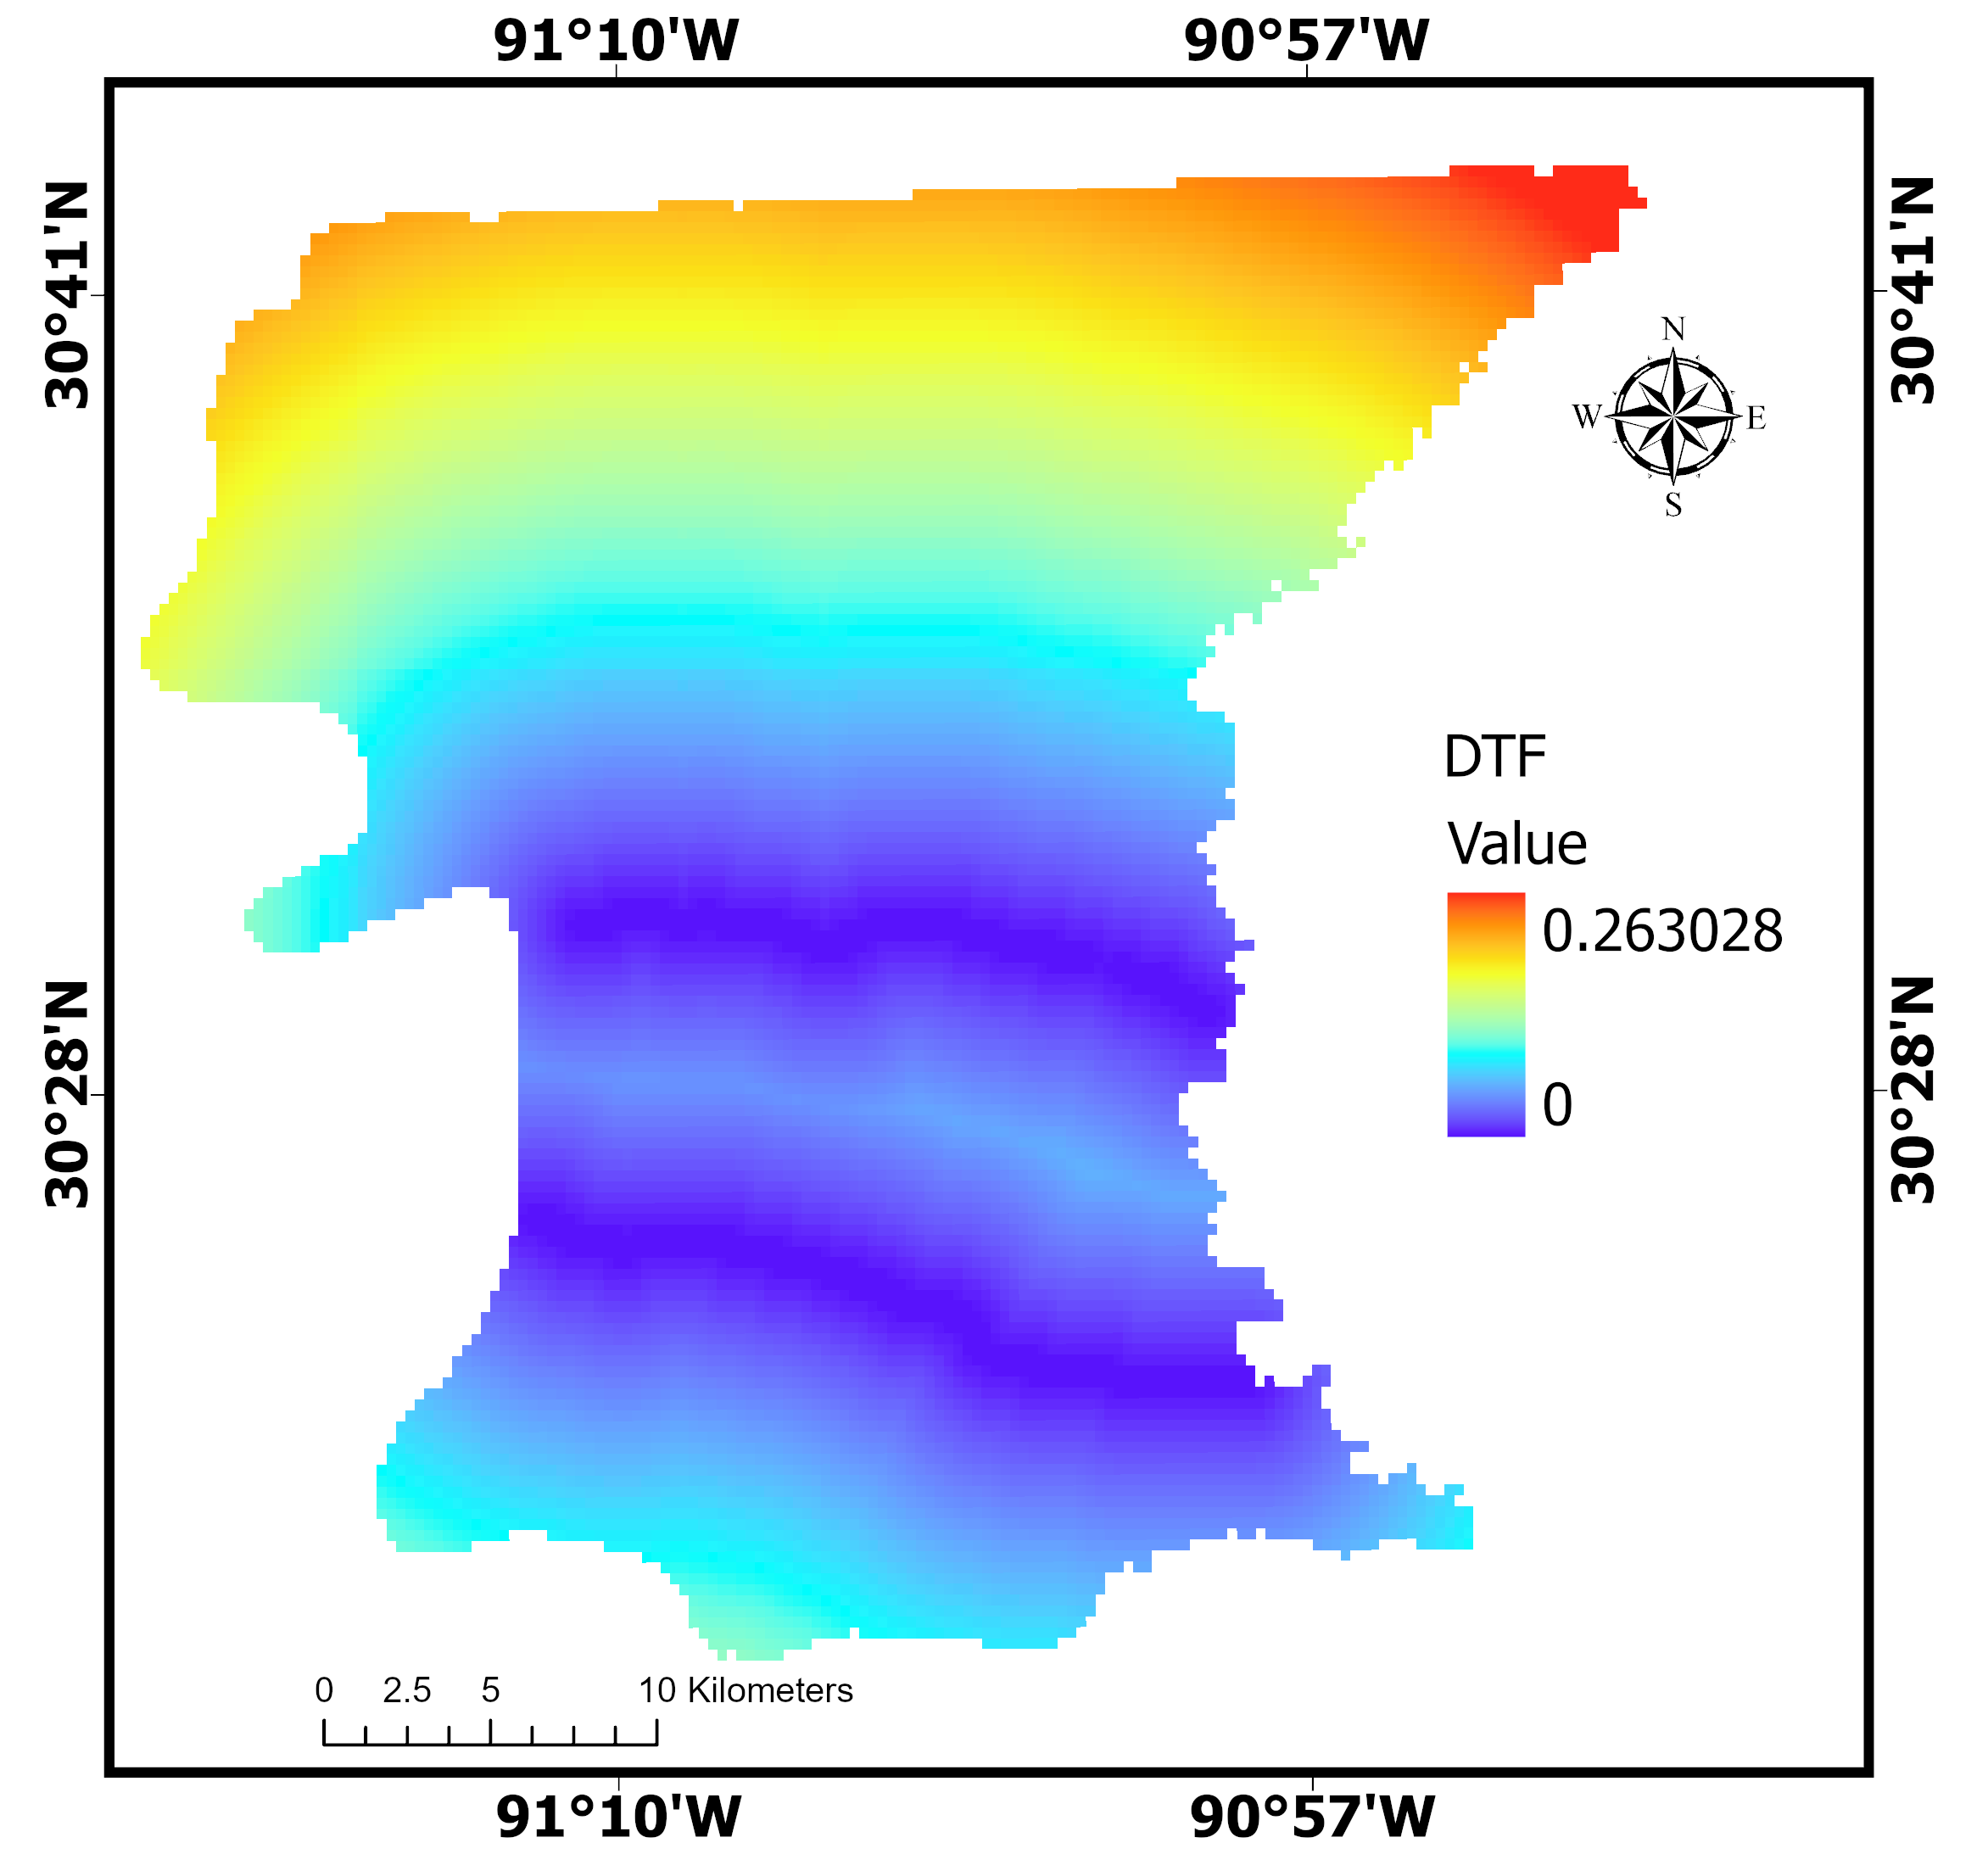
\includegraphics[width=0.48\textwidth]{All_layers/dtf.png} \\
(a) Distance to River & (b) Distance to Fault
\end{tabular}
\caption{Hydrological and structural conditioning factors}
\label{fig:hydro_struct_factors}
\end{figure}

\subsubsection{Infrastructure Factors}
Proximity to roads, railways, and bridges quantifies surface loading from built infrastructure (Figure~\ref{fig:infra_factors}).

\begin{figure}[htbp]
\centering
\begin{tabular}{ccc}
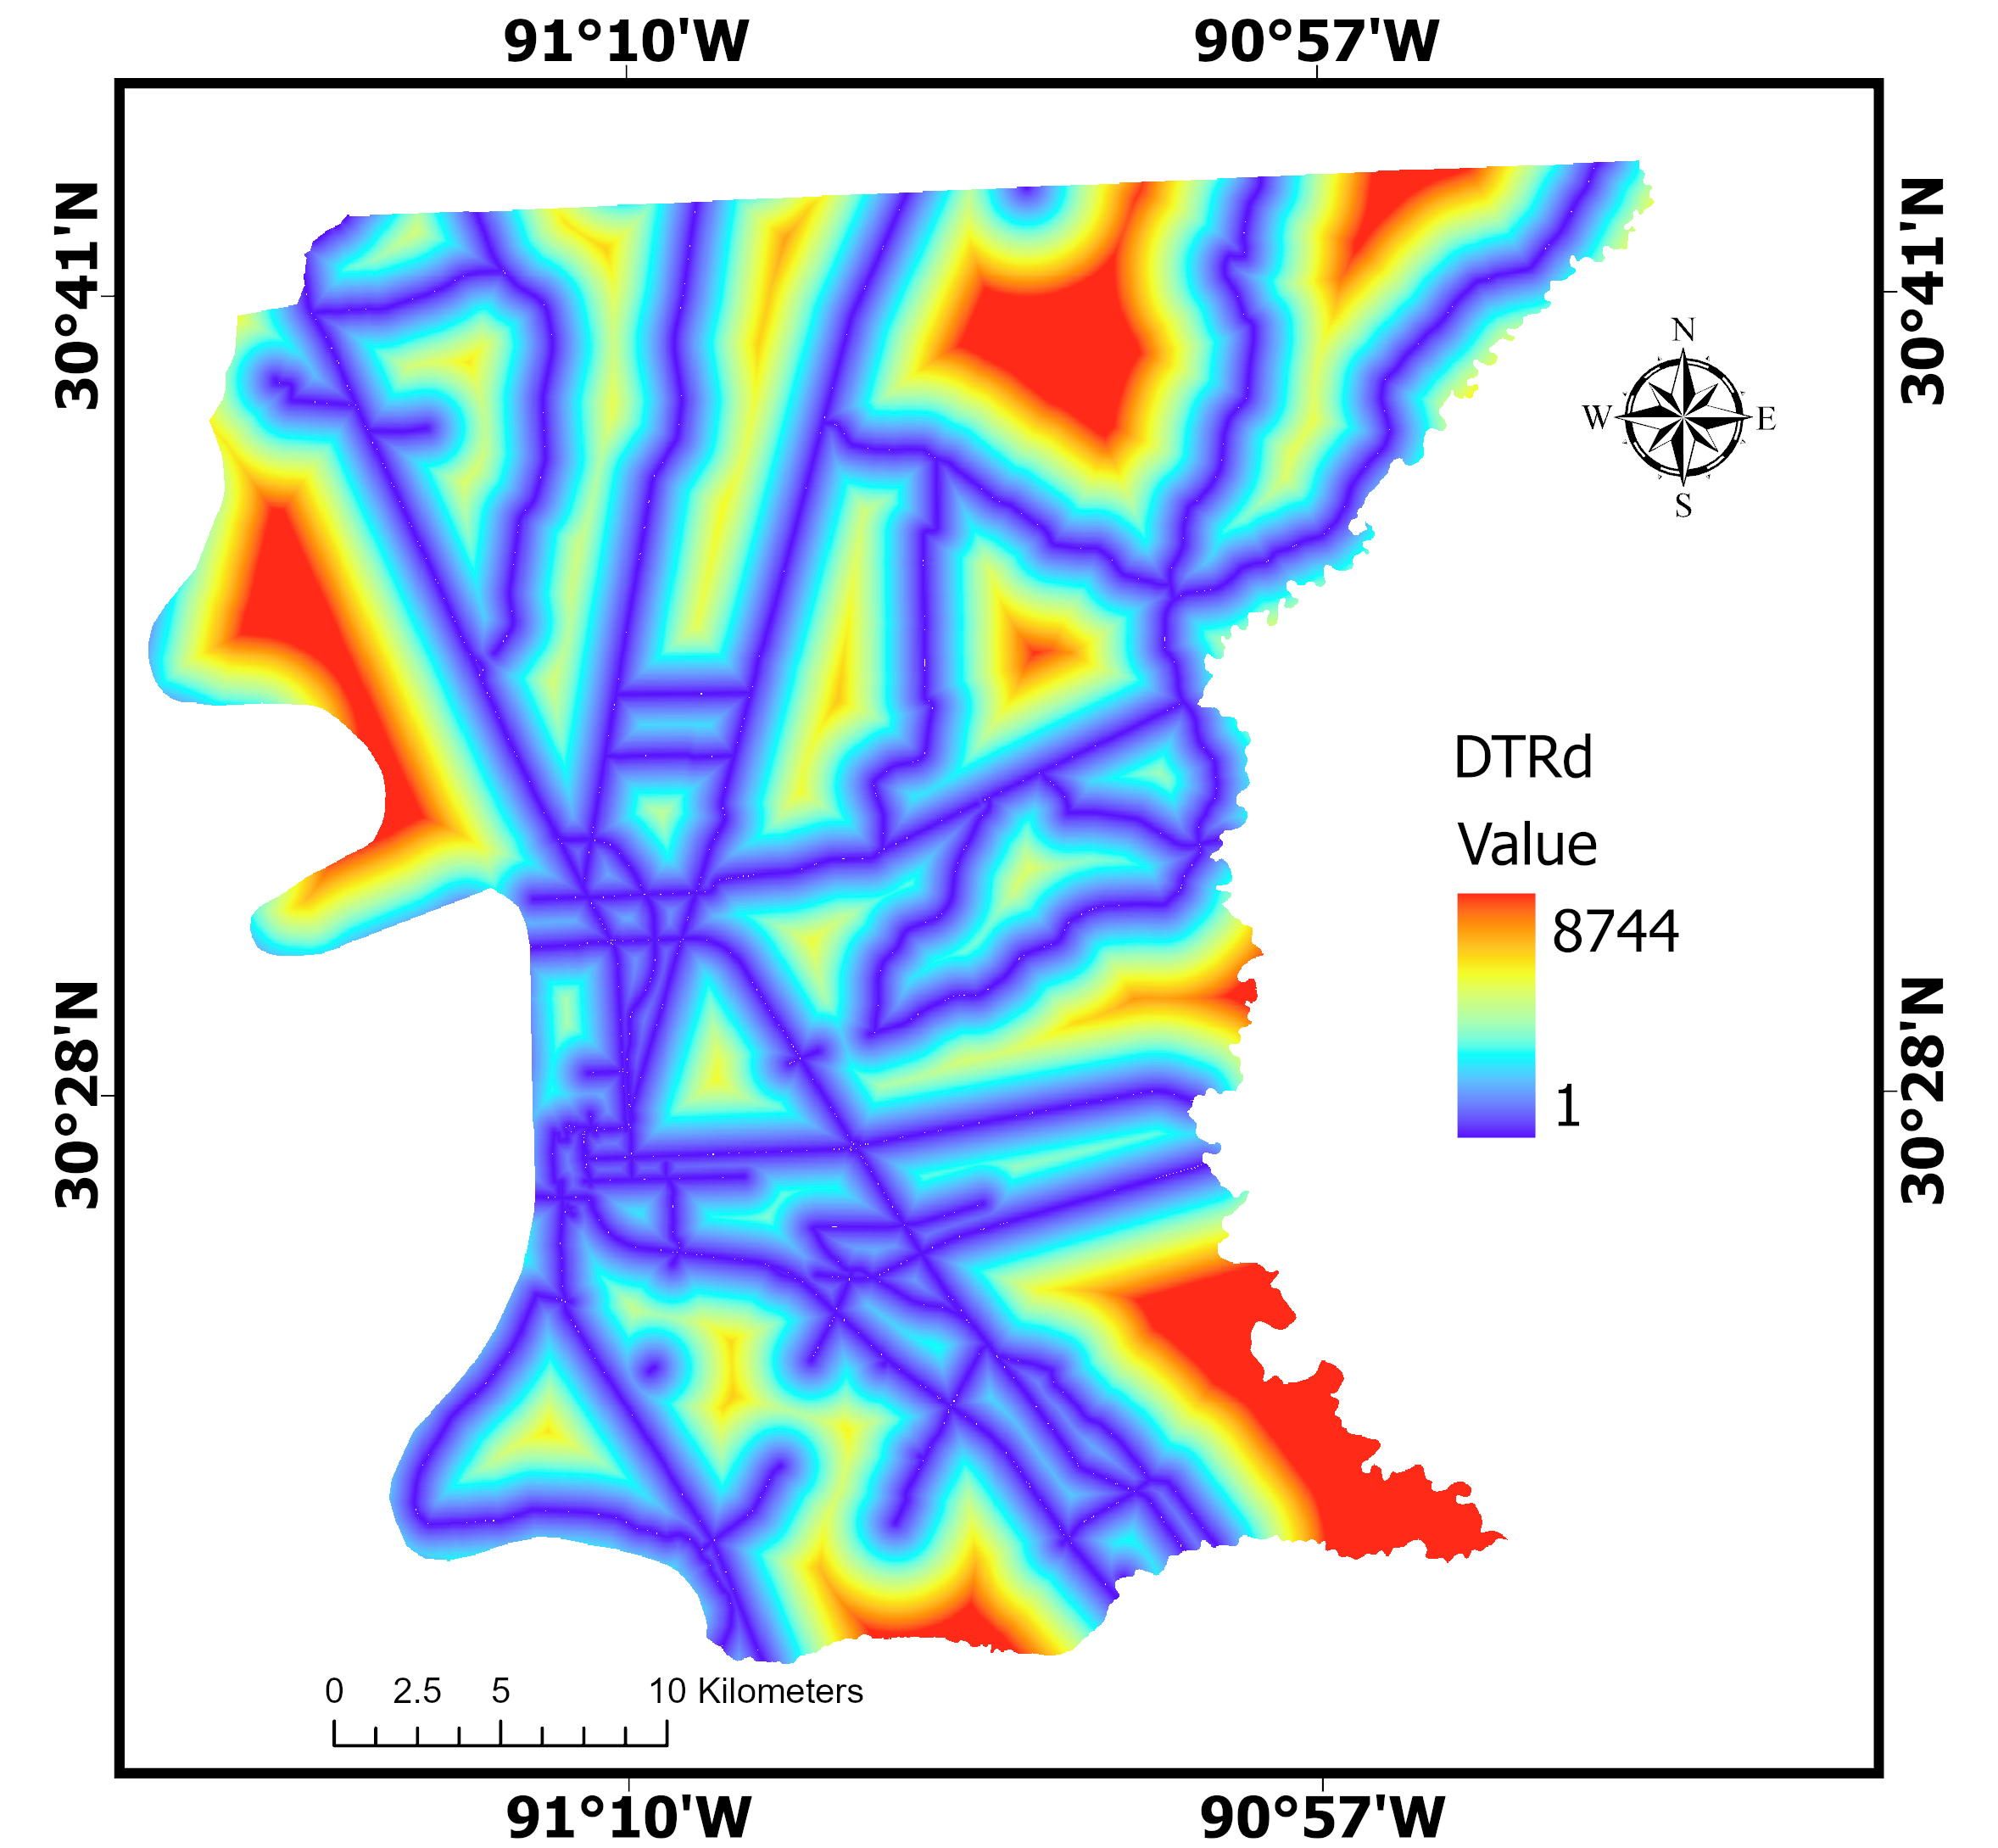
\includegraphics[width=0.32\textwidth]{All_layers/distancefrod.png} &
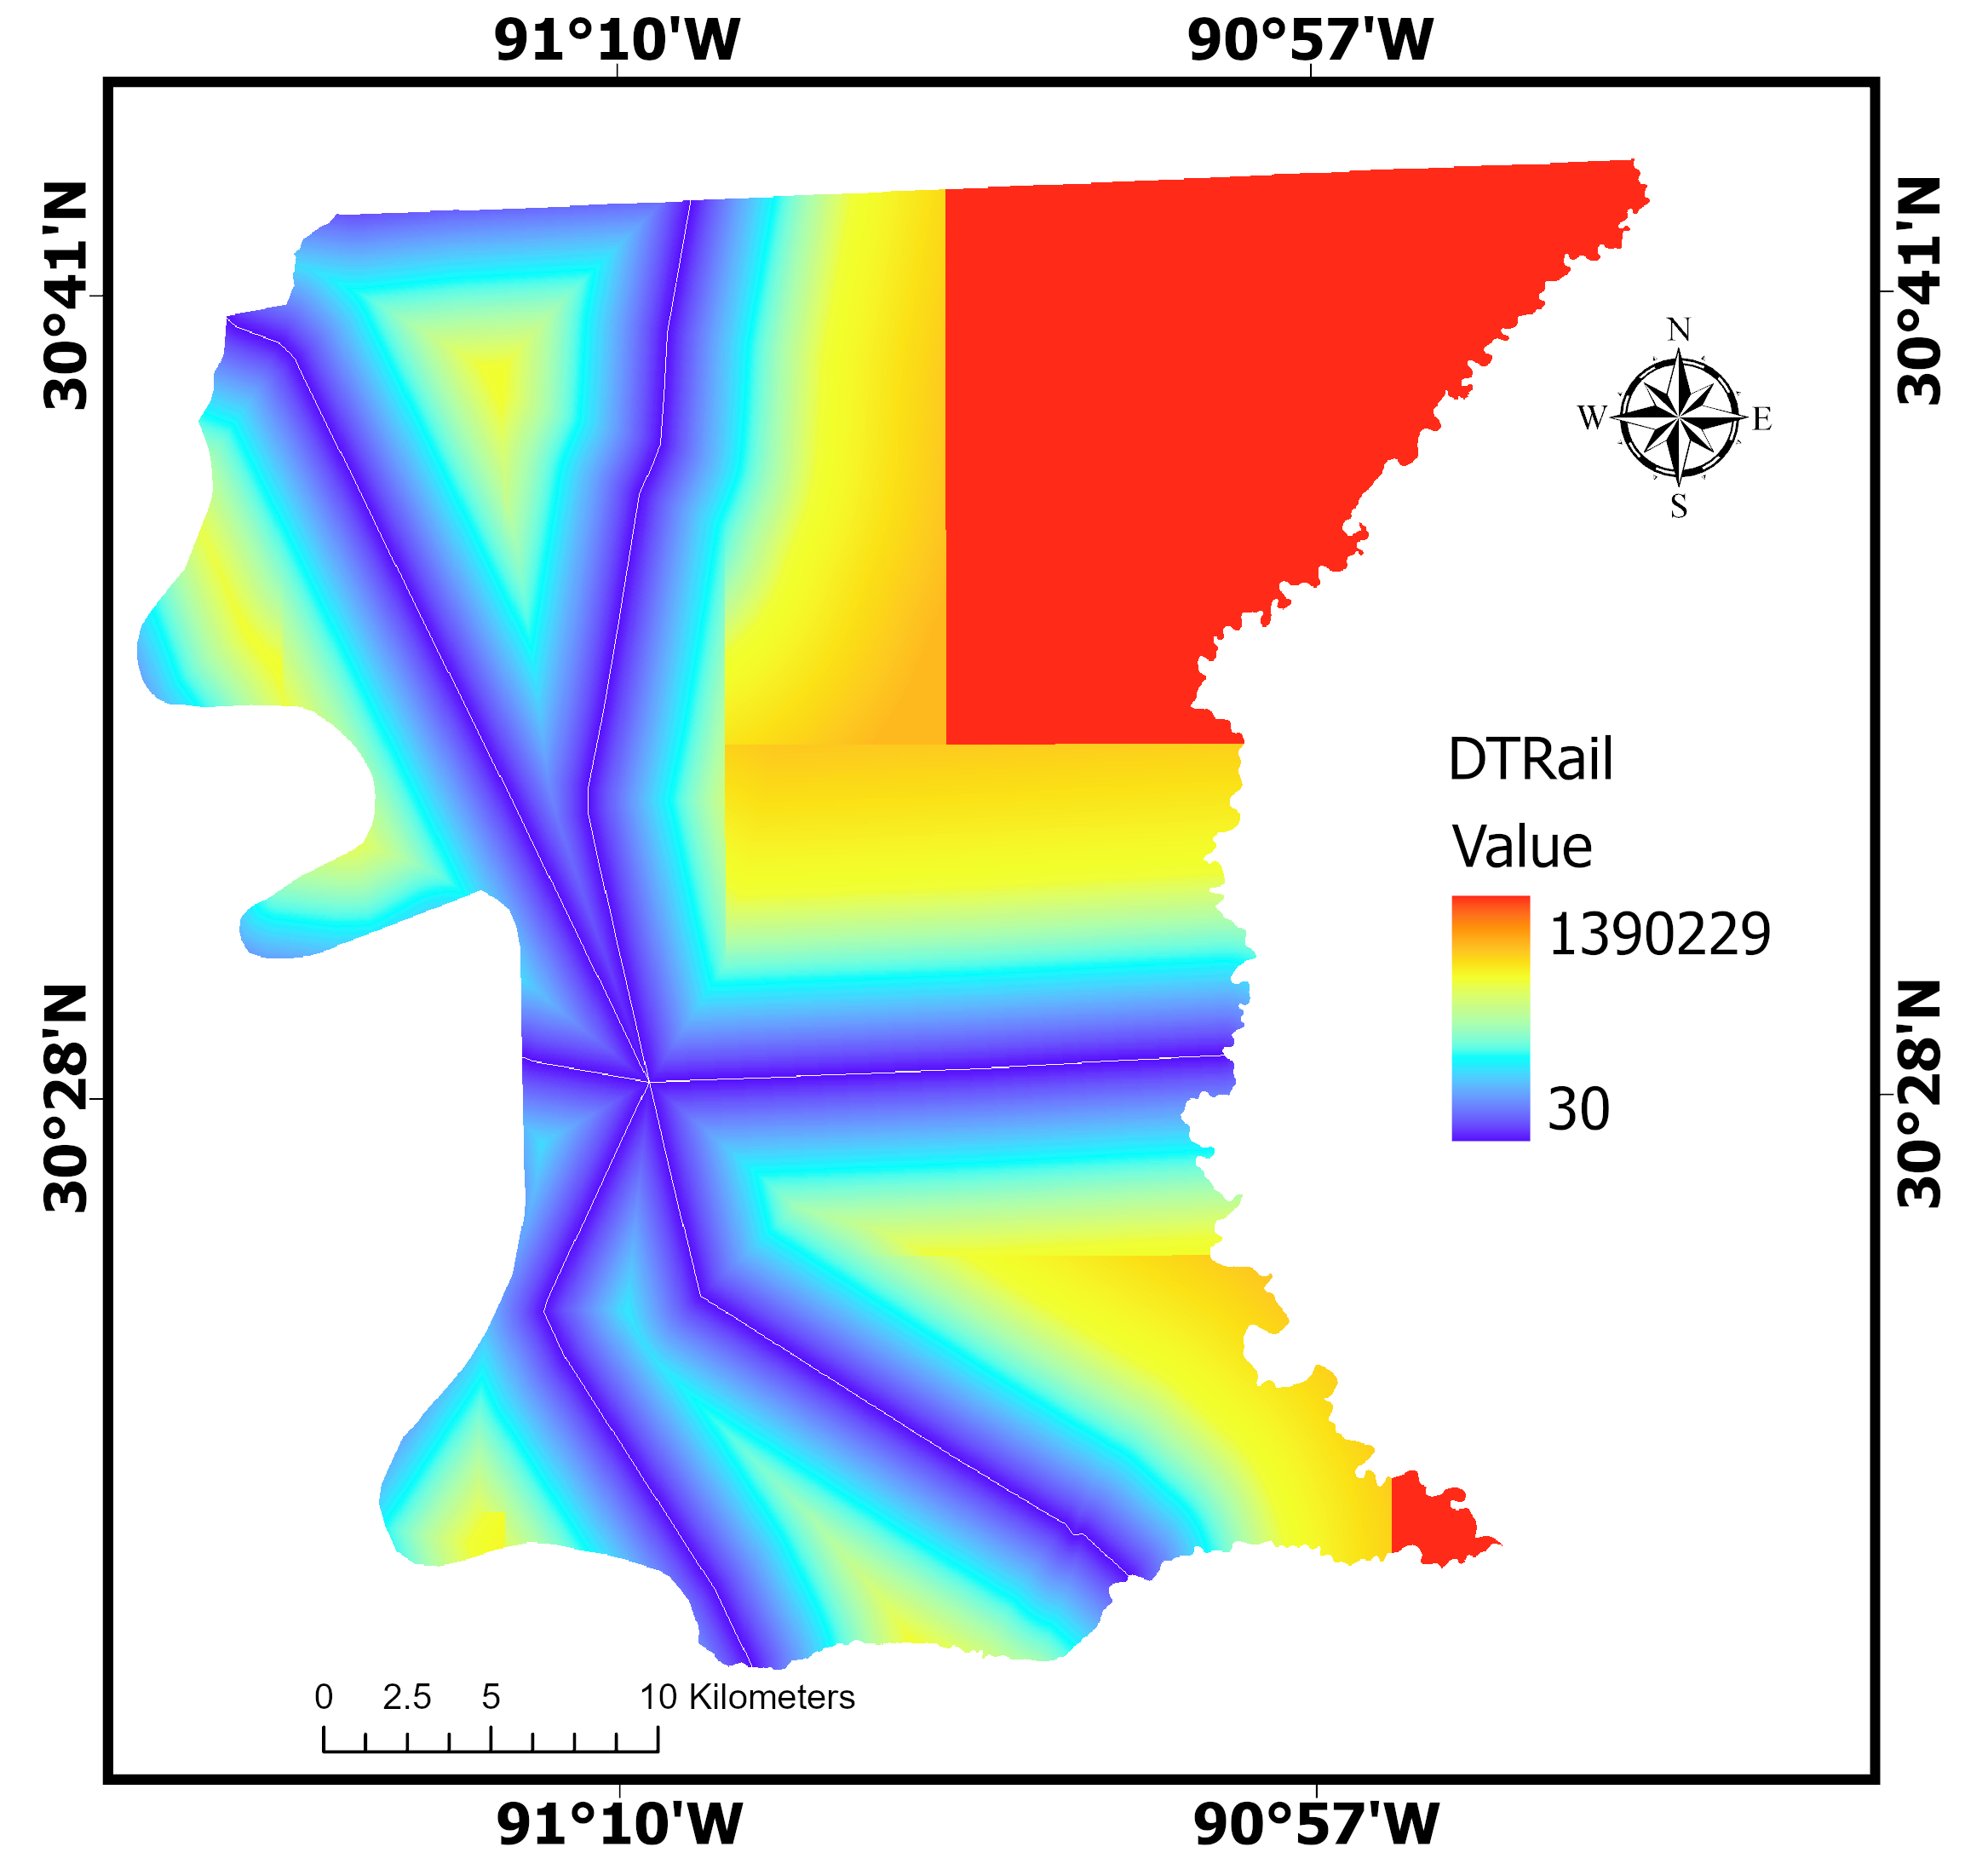
\includegraphics[width=0.32\textwidth]{All_layers/distancerail.png} &
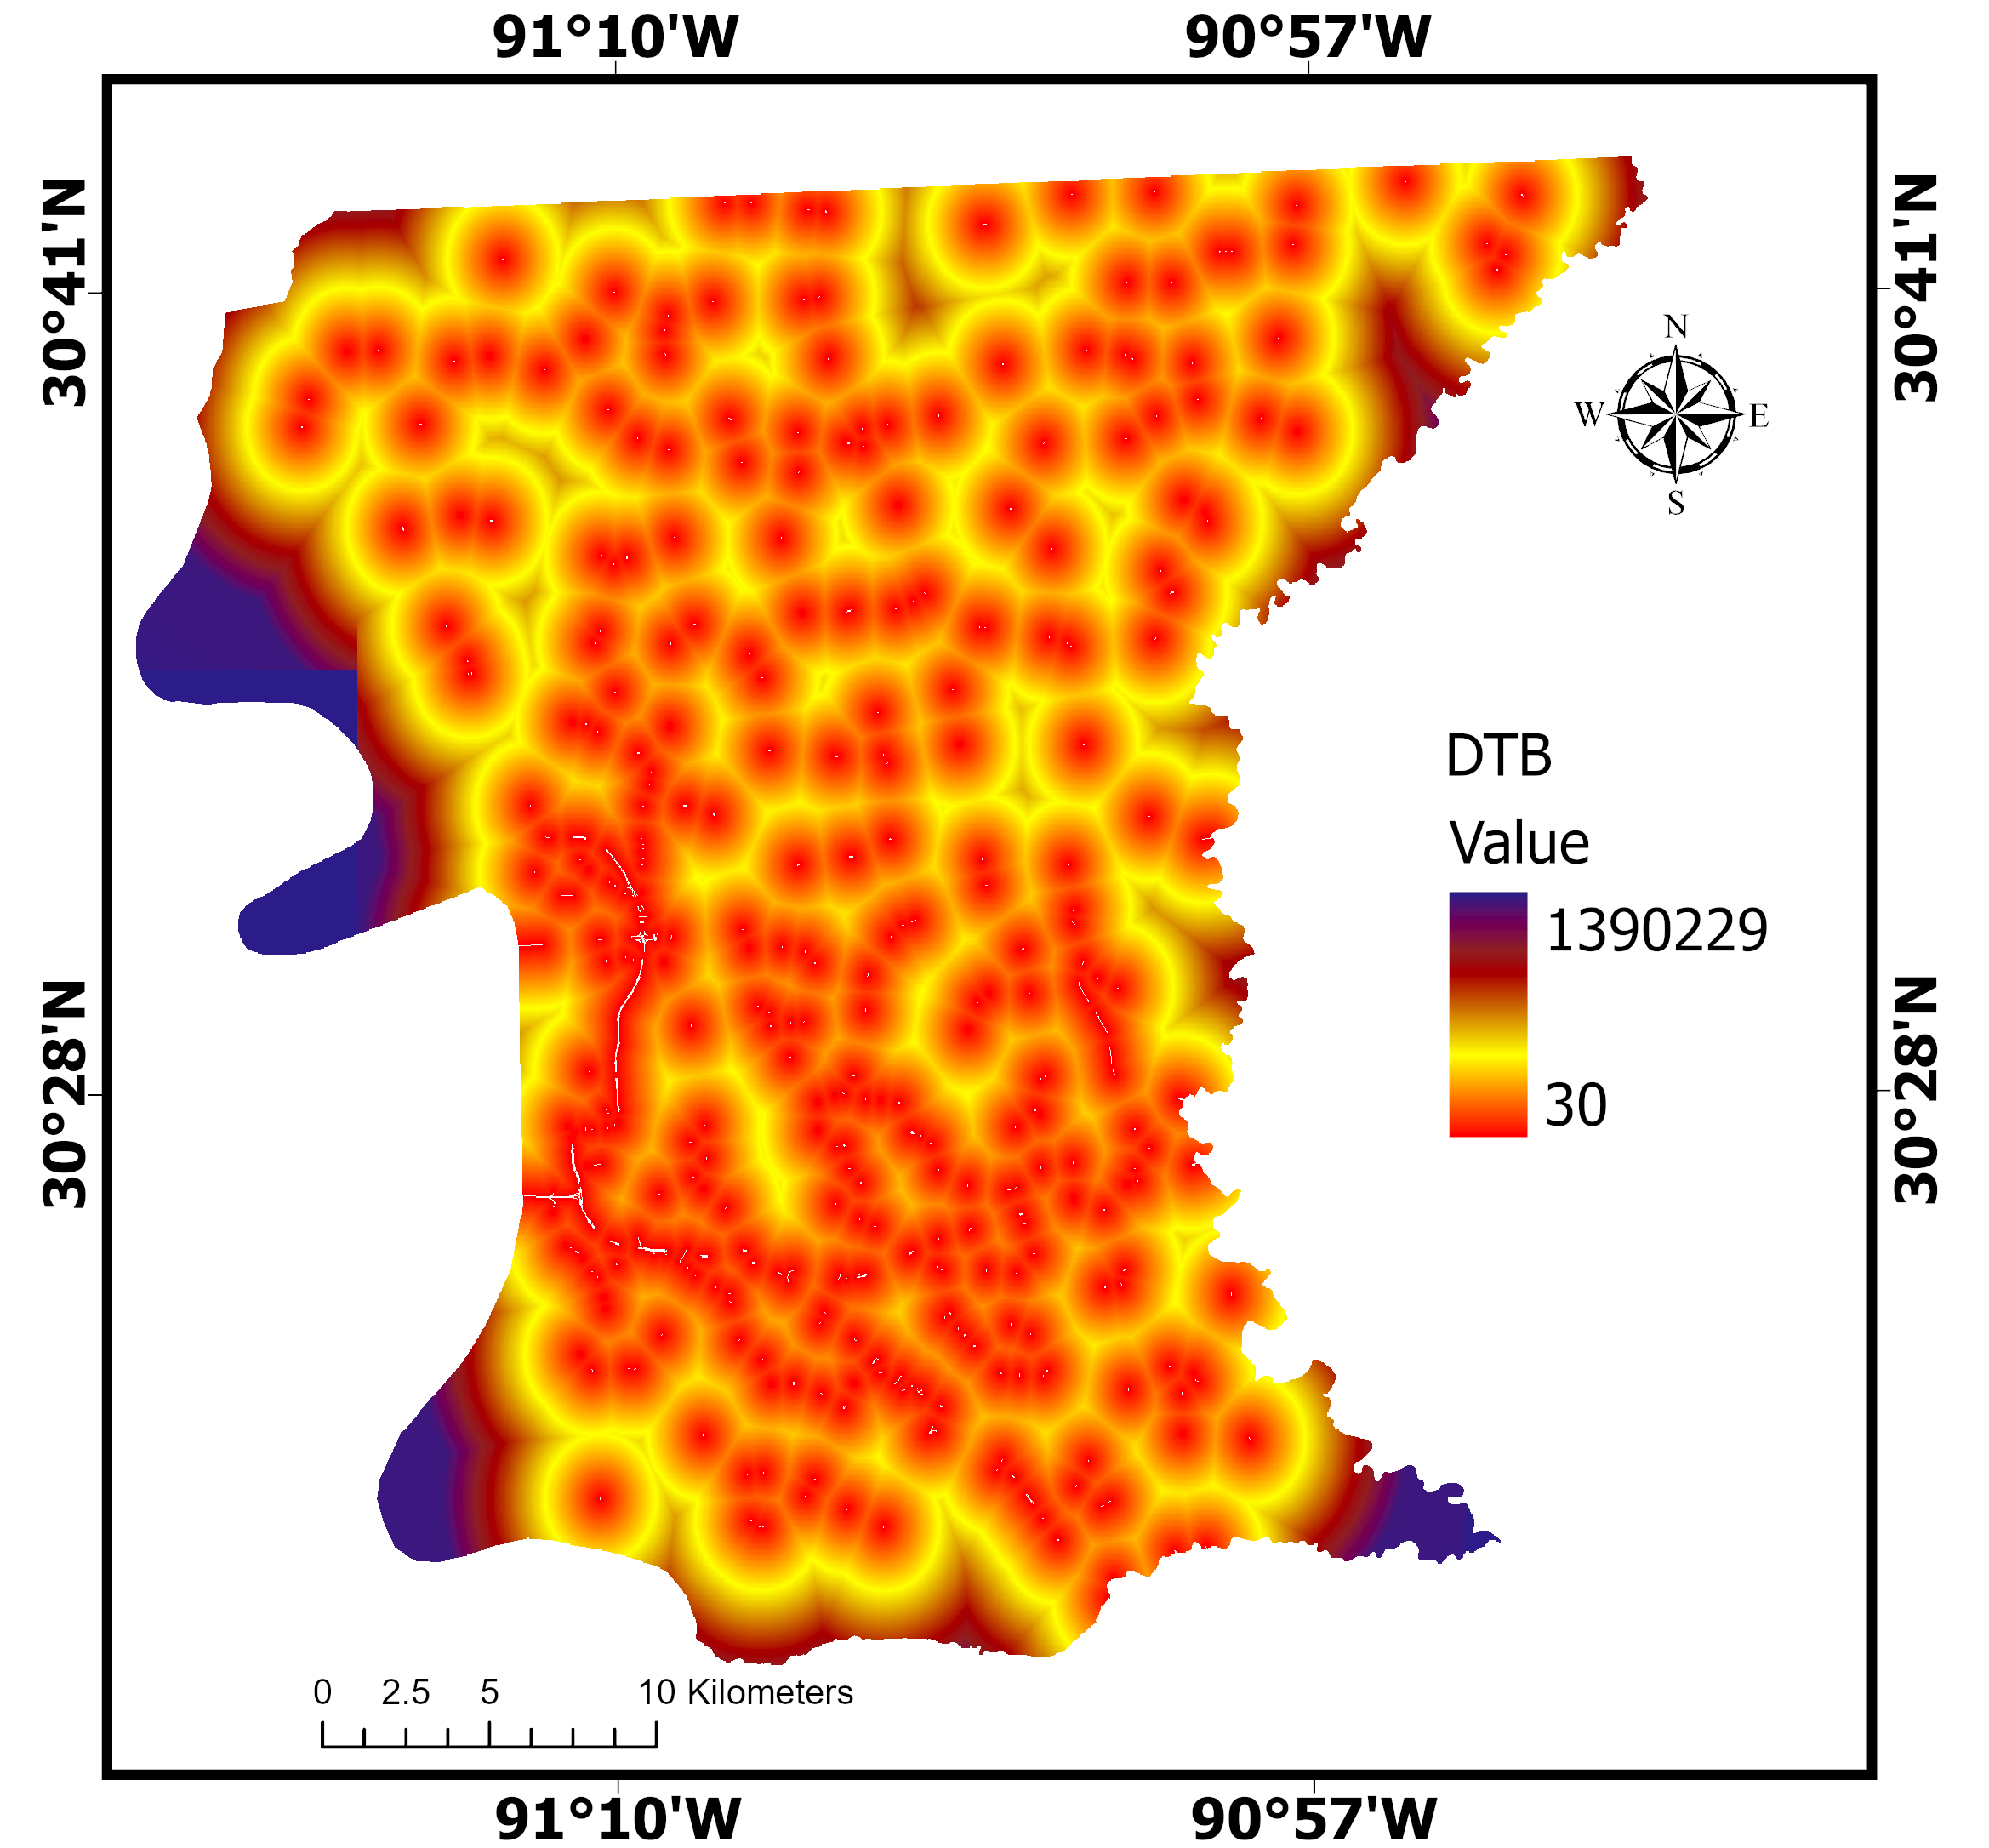
\includegraphics[width=0.32\textwidth]{All_layers/distancebridge.png} \\
(a) Distance to Road & (b) Distance to Railway & (c) Distance to Bridge
\end{tabular}
\caption{Infrastructure conditioning factors}
\label{fig:infra_factors}
\end{figure}

\subsubsection{Climatic and Anthropogenic Factors}
Precipitation represents climatic variability, while interpolated groundwater well influence (well\_idw) quantifies anthropogenic groundwater extraction patterns.

\begin{figure}[htbp]
\centering
\begin{tabular}{cc}
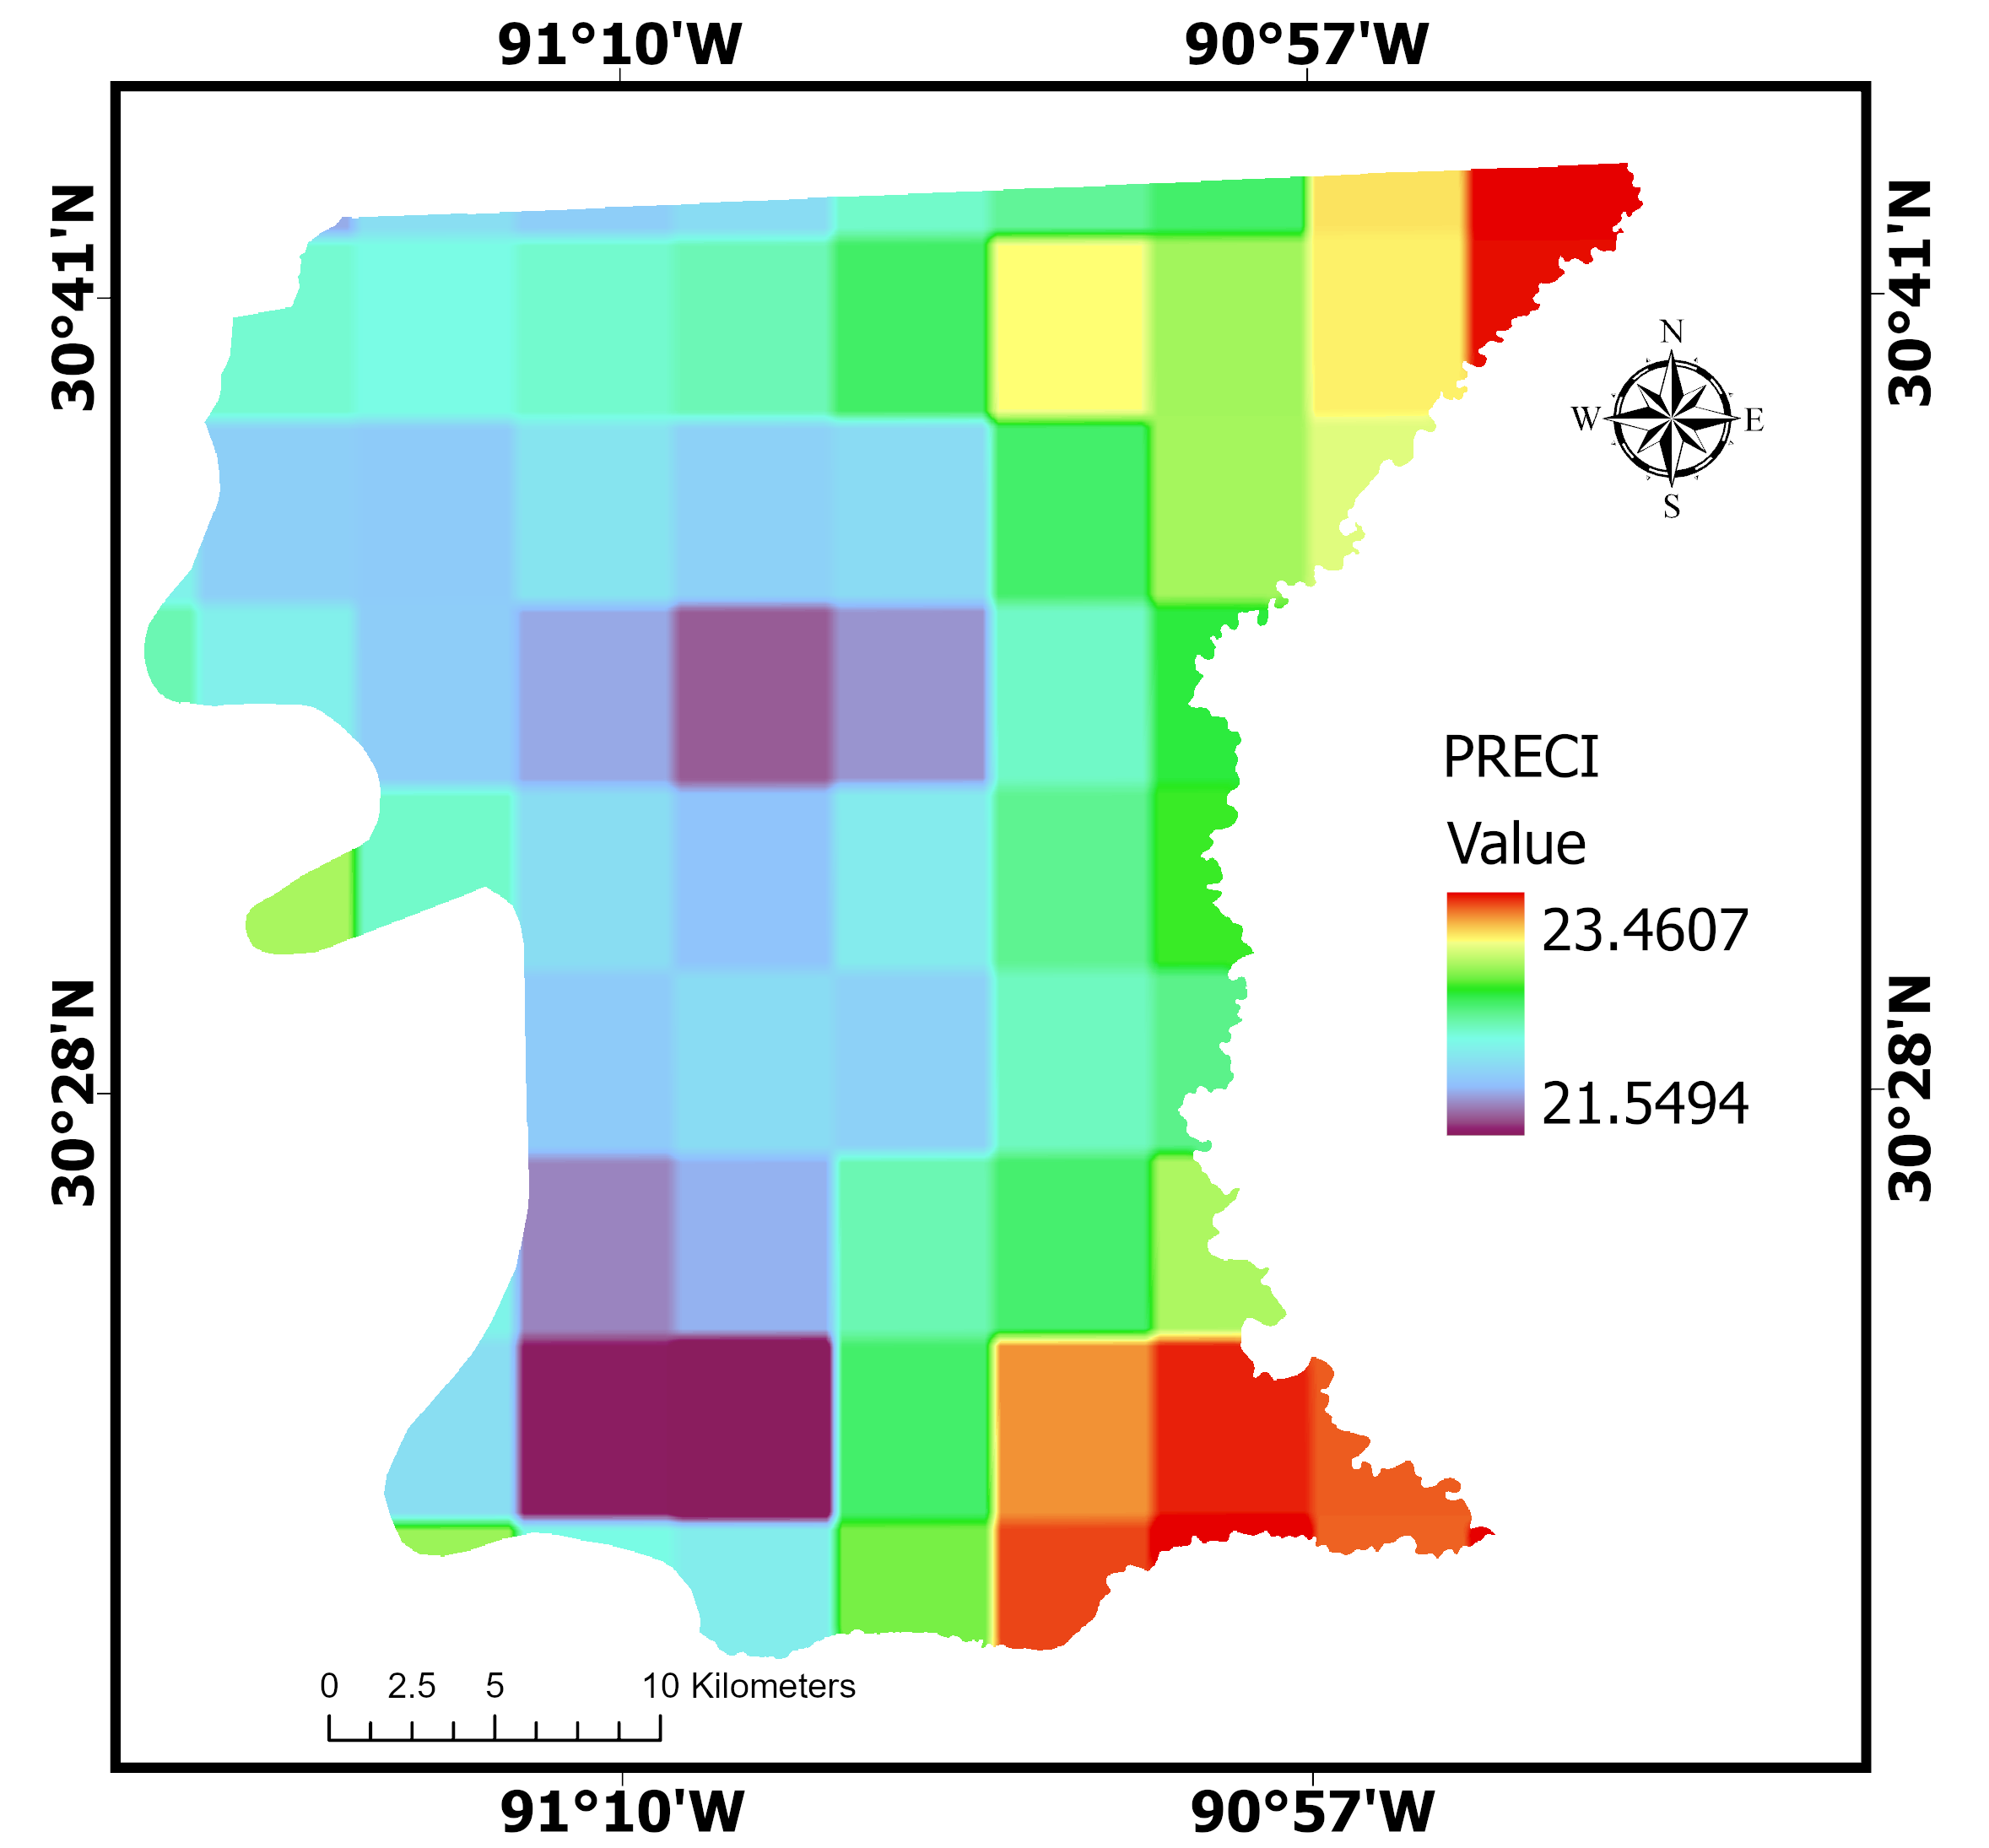
\includegraphics[width=0.48\textwidth]{All_layers/preci.png} &
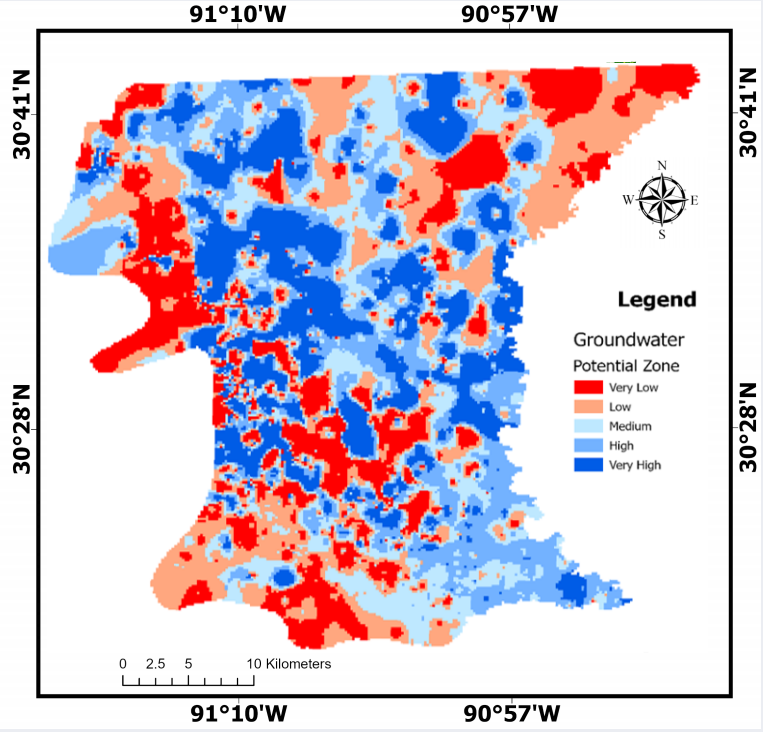
\includegraphics[width=0.48\textwidth]{All_layers/well.png} \\
(a) Precipitation & (b) Groundwater Well Influence
\end{tabular}
\caption{Climatic and anthropogenic conditioning factors}
\label{fig:anthro_factors}
\end{figure}

Continuous layers were min--max scaled to [0,1]; categorical layers (geology, LULC) were one-hot encoded.

\subsection{Validation Data}
InSAR-derived deformation was validated using GNSS vertical displacement time series
 from the GulfNet CORS stations (1LSU, GMVS and SJB1) in EBRP obtained from the Nevada Geodetic
 Laboratory (NGL). GNSS provides high-precision point-based measurements and serves as a 
 standard benchmark for InSAR timeseries validation \citep{Abdalla2024}.

Following the description of the study area and data sources, existing literature on 
InSAR monitoring and machine learning–based subsidence analysis is
reviewed to identify gaps that justify the proposed integrated approach

\chapter[Literature Review]{\centering Literature Review}

\section{Overview of Land Subsidence in Urban Areas}

Land subsidence, defined as the gradual or sudden downward movement of the Earth's surface, is increasingly recognized as a major global geohazard, with over 80\% of severe cases associated with aquifer compaction and groundwater withdrawal \citep{Higgins2016}. In rapidly urbanizing regions like the Lower Mississippi Basin, the interplay between shallow geology and heavy infrastructure growth intensifies surface deformation \citep{HosseinzadehLLand2024}. 
Urban environments are particularly susceptible due to the high density of man-made structures that act as static loads on compressible soil layers. Subsidence processes are fueled by excessive groundwater extraction, sediment consolidation, urban infrastructure loading, and land-use change \citep{Holzer1985}. Research demonstrates how shallow geology and infrastructure growth can intensify surface deformation and compaction in these regions \citep{ZouEtAl2016}.

Unmitigated subsidence triggers a cascade of secondary hazards, including diminished drainage capacity, heightened susceptibility to flooding in low-lying urban corridors, pipeline ruptures, building tilting, and structural failures, resulting in significant economic losses \citep{ZouEtAl2016}. Subsurface faulting and structural geology make subsidence patterns in many cities even more complex. 
These findings highlight the need for reliable frameworks that can both map the areas where subsidence is most likely to occur and predict its future course.

\section{Advancements in InSAR Monitoring for Subsidence}

Having established the severity and complexity of urban subsidence as a geohazard, this section reviews the evolution of InSAR techniques that enable spatially continuous monitoring at regional scales.

The development of InSAR has transformed ground-deformation monitoring by providing high-resolution, wide-area observations.
 Traditional geodetic techniques, such as GNSS and levelling, have historically provided precise point measurements but are limited by prohibitive costs and low spatial resolution.

\subsection{Evolution of InSAR Techniques for Subsidence Monitoring}
InSAR emerged in early 1990s as a transformative remote sensing technique capable of detecting ground deformation by 
exploiting phase differences between radar images acquired at different times. Because radar phase is sensitive to path-length changes on the order of millimetres, 
InSAR enables precise measurement of surface displacement over large spatial extents \citep{Jiang2023}.

Early applications relied on Differential InSAR (D-InSAR), which isolates deformation by subtracting topographic phase contributions using DEM. D-InSAR 
proved effective for mapping rapid and spatially coherent deformation associated with earthquakes and volcanic activity \citep{Li2022}. However, its 
application to long-term subsidence monitoring is limited by atmospheric phase delay, temporal decorrelation, orbital errors, and phase unwrapping ambiguities,
particularly over vegetated or urbanizing surfaces.

To overcome these limitations, PS-InSAR was introduced to exploit radar targets that remain phase-stable over long time periods,
such as buildings and exposed infrastructure \citep{Ferretti2001}. By analyzing large stacks of SAR acquisitions, PS-InSAR achieves sub-millimeter precision 
on built infrastructure \citep{Ferretti2001,Ferretti2011}. However, PS-InSAR is often sparse in non-urbanized or vegetated areas, limiting its applicability to mixed land-cover environments.

SBAS-InSAR has emerged as a superior alternative, particularly in regions mixed urban and vegetated terrain \citep{Berardino2002}. 
It was developed to improve spatial coverage by forming interferogram networks with short temporal timeseries reconstruction over distributed scatterers, 
making it particularly suitable for regions characterized by mixed land cover. 
By utilizing multiple master interferograms with small perpendicular baselines, SBAS identifies Slowly Decorrelating Filtered Pixels (SDFP), which significantly reduces the impact of spatial and temporal decorrelation.
Recent studies indicate that large-scale time-series data processing supports the identification of both linear and complex non-linear deformation behaviours with millimetre-level accuracy.
Comparatively, SBAS-InSAR provides up to 2.83 times higher monitoring density than PS-InSAR in mixed urban-rural environments \citep{Bayik2025}.

Although SBAS-InSAR generally exhibits lower point-wise precision than PS-InSAR, it provides dense and spatially continuous deformation fields essential for regional subsidence analysis \citep{Crosetto2016}.

Unlike traditional geodetic methods, InSAR enables millimeter-scale motion detection across vast regions regardless of weather or lighting conditions \citep{Crosetto2016}. Building on these advances, newer methods such as Distributed Scatterer (DS-InSAR) and Multi-Temporal InSAR (MT-InSAR) extend coherence to mixed urban--rural environments by statistically analyzing pixel clusters \citep{Fattahi2015}.

More recent approaches, including DS-InSAR and hybrid methods such as SqueeSAR, further extend coherence in low-reflectivity areas by statistically analysing homogeneous pixel clusters, enabling deformation monitoring in challenging environments where traditional methods fail \citep{Ferretti2011}.

\subsection{Temporal Decorrelation, Atmospheric Effects, and Time-Series Reliability}

Temporal decorrelation remains a fundamental challenge across all 
InSAR techniques, arising from changes in surface scattering properties caused by vegetation growth, soil moisture variation, and anthropogenic activity \citep{Zheng2024}.
In urban–natural transition zones, heterogeneous coherence leads to spatially variable uncertainty in deformation estimates.

Atmospheric phase delay, particularly tropospheric water vapour variability, introduces long-wavelength artefacts that can mimic real deformation signals.
These effects are especially pronounced in humid subtropical regions such as the U.S. Gulf Coast. Recent integration of numerical weather models and reanalysis products, including ERA5 and GACOS, has significantly improved atmospheric correction and time-series reliability, enabling more accurate long-term deformation trend detection \citep{HosseinzadehLLand2024}.

\section{Machine Learning for Subsidence Susceptibility Mapping}

Machine learning (ML) has become the global standard for modelling the non-linear relationship between ground deformation and various geospatial drivers, such as Land Use/Land Cover (LULC), soil types, and distance from faults. Common ML algorithms employed in geohazard susceptibility mapping include Random Forest (RF), K-Nearest Neighbors (KNN), and Classification and Regression Trees (CART). \citet{Gharechaee2023} applied RF, KNN, and CART to InSAR-derived subsidence in Iran's Bakhtegan Basin, finding RF performed best and highlighting that the leading susceptibility factors were not only groundwater withdrawal but also proximity to dams, faults and mines.

\subsection{Ensemble Learners Regression}

While Random Forest (RF) remains a common benchmark due to its ability to handle multi-variate data without pre-defined assumptions, 
it can be prone to overfitting in complex geological datasets \citep{Breiman2001}. This study identifies the Extremely Randomized Trees (ERT), also known as Extra Trees, as a more robust alternative for subsidence susceptibility mapping. By implementing random splits at the node level, ERT enhances model generalisation and reduces variance compared to conventional bagged ensembles \citep{Geurts2006}. \citet{HosseinzadehLLand2024} evaluated seven ML methods (CART, ERT, Support Vector Machine (SVM), RF, logistic regression, etc.) in Iran and found ERT outperformed others in susceptibility mapping. These studies demonstrate ML's strength in spatial patterning and factor ranking.
\subsection{Gaussian Process Regression and Data Augmentation}

Gaussian Process Regression (GPR) is increasingly used for its ability to model calibrated predictive uncertainty, making it highly effective for small datasets and areas with limited observability. To address the technical challenge of small dataset sizes in local subsidence surveys, Gaussian noise-based data augmentation has been validated as an effective strategy to expand training samples and ensure model stability \citep{Shorten2019}. This augmentation approach mitigates data gaps and enhances model generalization by expanding the effective training dataset.

\section{Deep Learning and Time Series Forecasting of Subsidence}

Deep-learning (DL) models, especially sequence models like LSTM, are increasingly adopted for subsidence forecasting because of their ability to capture temporal dependencies and non-linear dynamics. \citet{Li2020} applied LSTM to PS-InSAR data in Beijing Plain, showing promise for temporal modelling though with limitations in spatial generalization. \citet{Mirmazloumi2023} used LSTM on InSAR time-series for three mining sites, demonstrating an early-warning capability by forecasting 3--5 steps ahead.

\subsection{Physics-Informed Neural Networks (PINNs)}

Purely data-driven models may produce physically implausible results, such as unrealistic acceleration or velocity reversals. Physics-Informed Machine Learning (PIML) frameworks integrate geophysical constraints (e.g., velocity continuity and conservation laws) to ensure that long-term projections remain geomechanically consistent. \citet{Raissi2019} developed Physics-Informed Neural Networks (PINNs), which encode physical laws as penalty terms in the loss function, thereby constraining the model to produce physically realistic predictions. Such gaps suggest the potential for stacked models using meta-learning ensembles to combine base-model predictions and latent features for enhanced accuracy and interpretability. Hybrid models are common in other geohazard domains (e.g., landslides, groundwater) but remain under-utilized in urban subsidence. Thus, implementing a hybrid DL/ML ensemble to both map and forecast subsidence fills a methodological gap in current literature.

\section{Subsidence Driving Factor Analysis and Explainability}

A critical limitation of traditional deep learning is its ``black-box'' nature, which hinders its use in urban planning and policy-making. Explainable AI (XAI) techniques have emerged as essential tools for interpreting complex machine learning models and providing transparent insights into the decision-making processes of predictive algorithms \citep{Mohammadifar2021}. These methods enable researchers and practitioners to understand not only what a model predicts but also why specific predictions are made, thereby fostering trust and facilitating domain-specific insights in geohazard applications.

\subsection{SHapley Additive exPlanations (SHAP)}
SHAP is a cumulative feature attribution algorithm rooted in cooperative game theory that assigns a relevance score to each input feature \citep{Lundberg2017}. The method leverages concepts from Shapley values to calculate feature importance while satisfying key properties of feature attribution, including accuracy, missingness, and consistency. SHAP quantifies the marginal contribution of each feature by comparing model predictions with and without that feature across all possible feature combinations, providing a theoretically grounded measure of feature influence.

SHAP has been widely adopted in subsidence studies due to its ability to provide both global understanding of datasets through overall feature contributions and local explanations for individual predictions \citep{Gholami2023}. Recent applications include \citet{yu_explainable_2025}, who employed SHAP to interpret XGBoost-LightGBM-CatBoost ensemble models for land subsidence susceptibility mapping in Hangzhou, demonstrating that engineering activities and soft soil distribution are the most influential factors.

\subsection{Local Interpretable Model-agnostic Explanations (LIME)}

LIME is a post-hoc XAI method that provides local explanations by approximating complex models with interpretable surrogate models in the vicinity of individual predictions \citep{Ribeiro2016}. Unlike SHAP, which derives from game-theoretic principles, LIME constructs locally faithful linear models by perturbing input features and observing the resulting prediction changes. This approach enables interpretation of any machine learning model, regardless of its underlying architecture.

In geohazard susceptibility mapping, LIME has been applied alongside SHAP to provide complementary perspectives on model behavior \citep{Prendin2023}. While SHAP offers theoretically grounded global and local attributions, LIME provides intuitive local approximations that can be particularly useful for explaining individual high-risk predictions to stakeholders. However, SHAP is generally preferred in subsidence studies because it provides a more comprehensive and fair assessment of feature importance, handles feature interactions explicitly, and offers superior visualizations including bee swarm plots and interaction matrices \citep{Armaghani2025}.

\subsection{Mean Decrease in Impurity (MDI) and Permutation Feature Importance}

Tree-based ensemble methods such as Random Forest and Extra Trees provide intrinsic feature importance measures through Mean Decrease in Impurity (MDI), also known as Gini importance \citep{Breiman2001}. MDI scores are computed based on the average reduction in impurity associated with a feature across all nodes of the decision trees. This method exploits the interpretable nature of random forests to rank features as a byproduct of the trained model, indicating the extent to which specific features influence model outputs on average \citep{Abdalla2024}.

Permutation Feature Importance (PFI) offers an alternative approach by measuring the decrease in model performance when feature values are randomly shuffled \citep{Molnar2022}. Unlike MDI, which is specific to tree-based models, PFI is model-agnostic and can be applied to any predictive algorithm. Both MDI and PFI were utilized in recent coastal subsidence studies to estimate global feature importance, with results compared against SHAP-derived attributions to ensure robust driver identification \citep{Abdalla2024}.

\subsection{Integration of Explainability in Subsidence Analysis}

Recent studies demonstrate the value of combining multiple explainability approaches for robust driver identification. \citet{Mohammadifar2021} combined PFIM with SHAP, while \citet{Abdalla2024} employed MDI, PFI, and Kernel SHAP for comprehensive driver attribution in coastal subsidence analysis. The integration of SHAP with LIME provides complementary global and local interpretability, with SHAP offering theoretically consistent feature attributions and LIME providing intuitive instance-level explanations \citep{Armaghani2025}. MDI from tree-based models serves as an efficient baseline for feature ranking, which can be validated against SHAP-derived attributions. These integrated approaches support mitigation strategies and policy decisions by revealing that LULC, fault proximity, and groundwater fluctuations are primary contributors to regional deformation \citep{Maluleka2025}. However, few investigations combine hybrid DL forecasting with explicit causative-factor analysis using SHAP, LIME, and MDI in urban contexts, representing a key literature gap.

\section{Data Scarcity and Augmentation Techniques}

In geohazard research, obtaining large datasets for model training is often time-consuming and expensive. Gaussian noise-based data augmentation is a validated strategy to improve model stability and generalisation.
 Adding small amounts of noise allows the training set to expand significantly without distorting the original data distribution, thereby preventing overfitting in tree-based and deep-learning architectures. 
 This approach has been successfully applied in the context of subsidence prediction with Extra Trees models, where synthetic data generation improved model robustness without compromising prediction accuracy \citep{Shorten2019}.

\section{Research Gaps and Study Objectives}

While many studies have applied InSAR and machine or deep learning (ML/DL) methods to analyze land subsidence, most have treated spatial susceptibility mapping and temporal forecasting as separate tasks, often overlooking model interpretability \citep{Gharechaee2023, Rahmani2024}.
Applications within complex U.S. Gulf Coast urban environments also remain limited. Recent research by \citet{HeEtAl2025} highlighted the specific need for integrated monitoring and assessment frameworks in coastal subsidence-prone regions. 
To address these gaps, this study integrates SBAS-InSAR velocity data with environmental conditioning factors using Extra Trees and Random Forest for spatial subsidence susceptibility mapping, alongside a physics-informed LSTM framework for temporal forecasting. 
SHAP-based interpretation is employed to develop predictive and explainable subsidence models tailored to Baton Rouge's environmental and infrastructural characteristics \citep{Abdalla2024, Mojtahedi2025}.

The identified gaps and methodological advances reviewed in this chapter provide the foundation for the integrated approach detailed in Chapter 4, which combines SBAS-InSAR, ensemble machine learning, and physics-informed temporal forecasting to address subsidence monitoring and prediction in East Baton Rouge Parish.

\chapter[Methods]{\centering Methods}

This chapter details the integrated framework employed to map and forecast land subsidence in EBRP (Figure~\ref{fig:methodology_flowchart}). The methodology combines three complementary approaches: (1) SBAS-InSAR time-series analysis to extract deformation velocity from 246 Sentinel-1 acquisitions, (2) tree-based ensemble learning (RF and ERT) for spatial susceptibility mapping using 15 environmental conditioning factors, and (3) physics-informed LSTM networks for spatio-temporal forecasting. 
SHAP and LIME-based explainability are integrated with MDI to identify dominant subsidence drivers and ensure model interpretability.

\section{SBAS-InSAR Processing}
SBAS-InSAR was selected over PS-InSAR for this study due to the mixed urban-rural land cover characteristics of East Baton Rouge Parish. While PS-InSAR achieves higher point-wise precision on stable infrastructure, it provides sparse coverage in vegetated and agricultural areas \citep{Ferretti2011}. SBAS-InSAR, by contrast, exploits distributed scatterers and maintains coherence across heterogeneous terrain, yielding 2.83 times higher spatial density in mixed environments \citep{Bayik2025}. This enhanced coverage is critical for regional subsidence mapping and for generating sufficient training samples for machine learning models.


SBAS-InSAR represents a widely adopted time-series InSAR methodology, initially introduced by \citet{Berardino2002}. This technique is frequently employed for large-scale urban monitoring applications.
The fundamental principle involves constructing a network of interferometric pairs characterized by minimal temporal and spatial baseline separations derived from the spatial distribution of SAR imagery. 
This approach as shown in Figure \ref{fig:methodology_flowchart} facilitates interferogram generation while minimizing decoherence and topographic phase errors. Time-series analysis is subsequently conducted to derive surface deformation information. When $M$ interferograms are generated from $N+1$ SAR acquisitions, a specific correlation exists between $M$ and $N$. The constraint governing this relationship is expressed as \citep{Colesanti2003}:
\begin{equation}
\frac{N+1}{2} \leq M \leq N \frac{N+1}{2}
\end{equation}

\begin{figure}[!t]
\centering
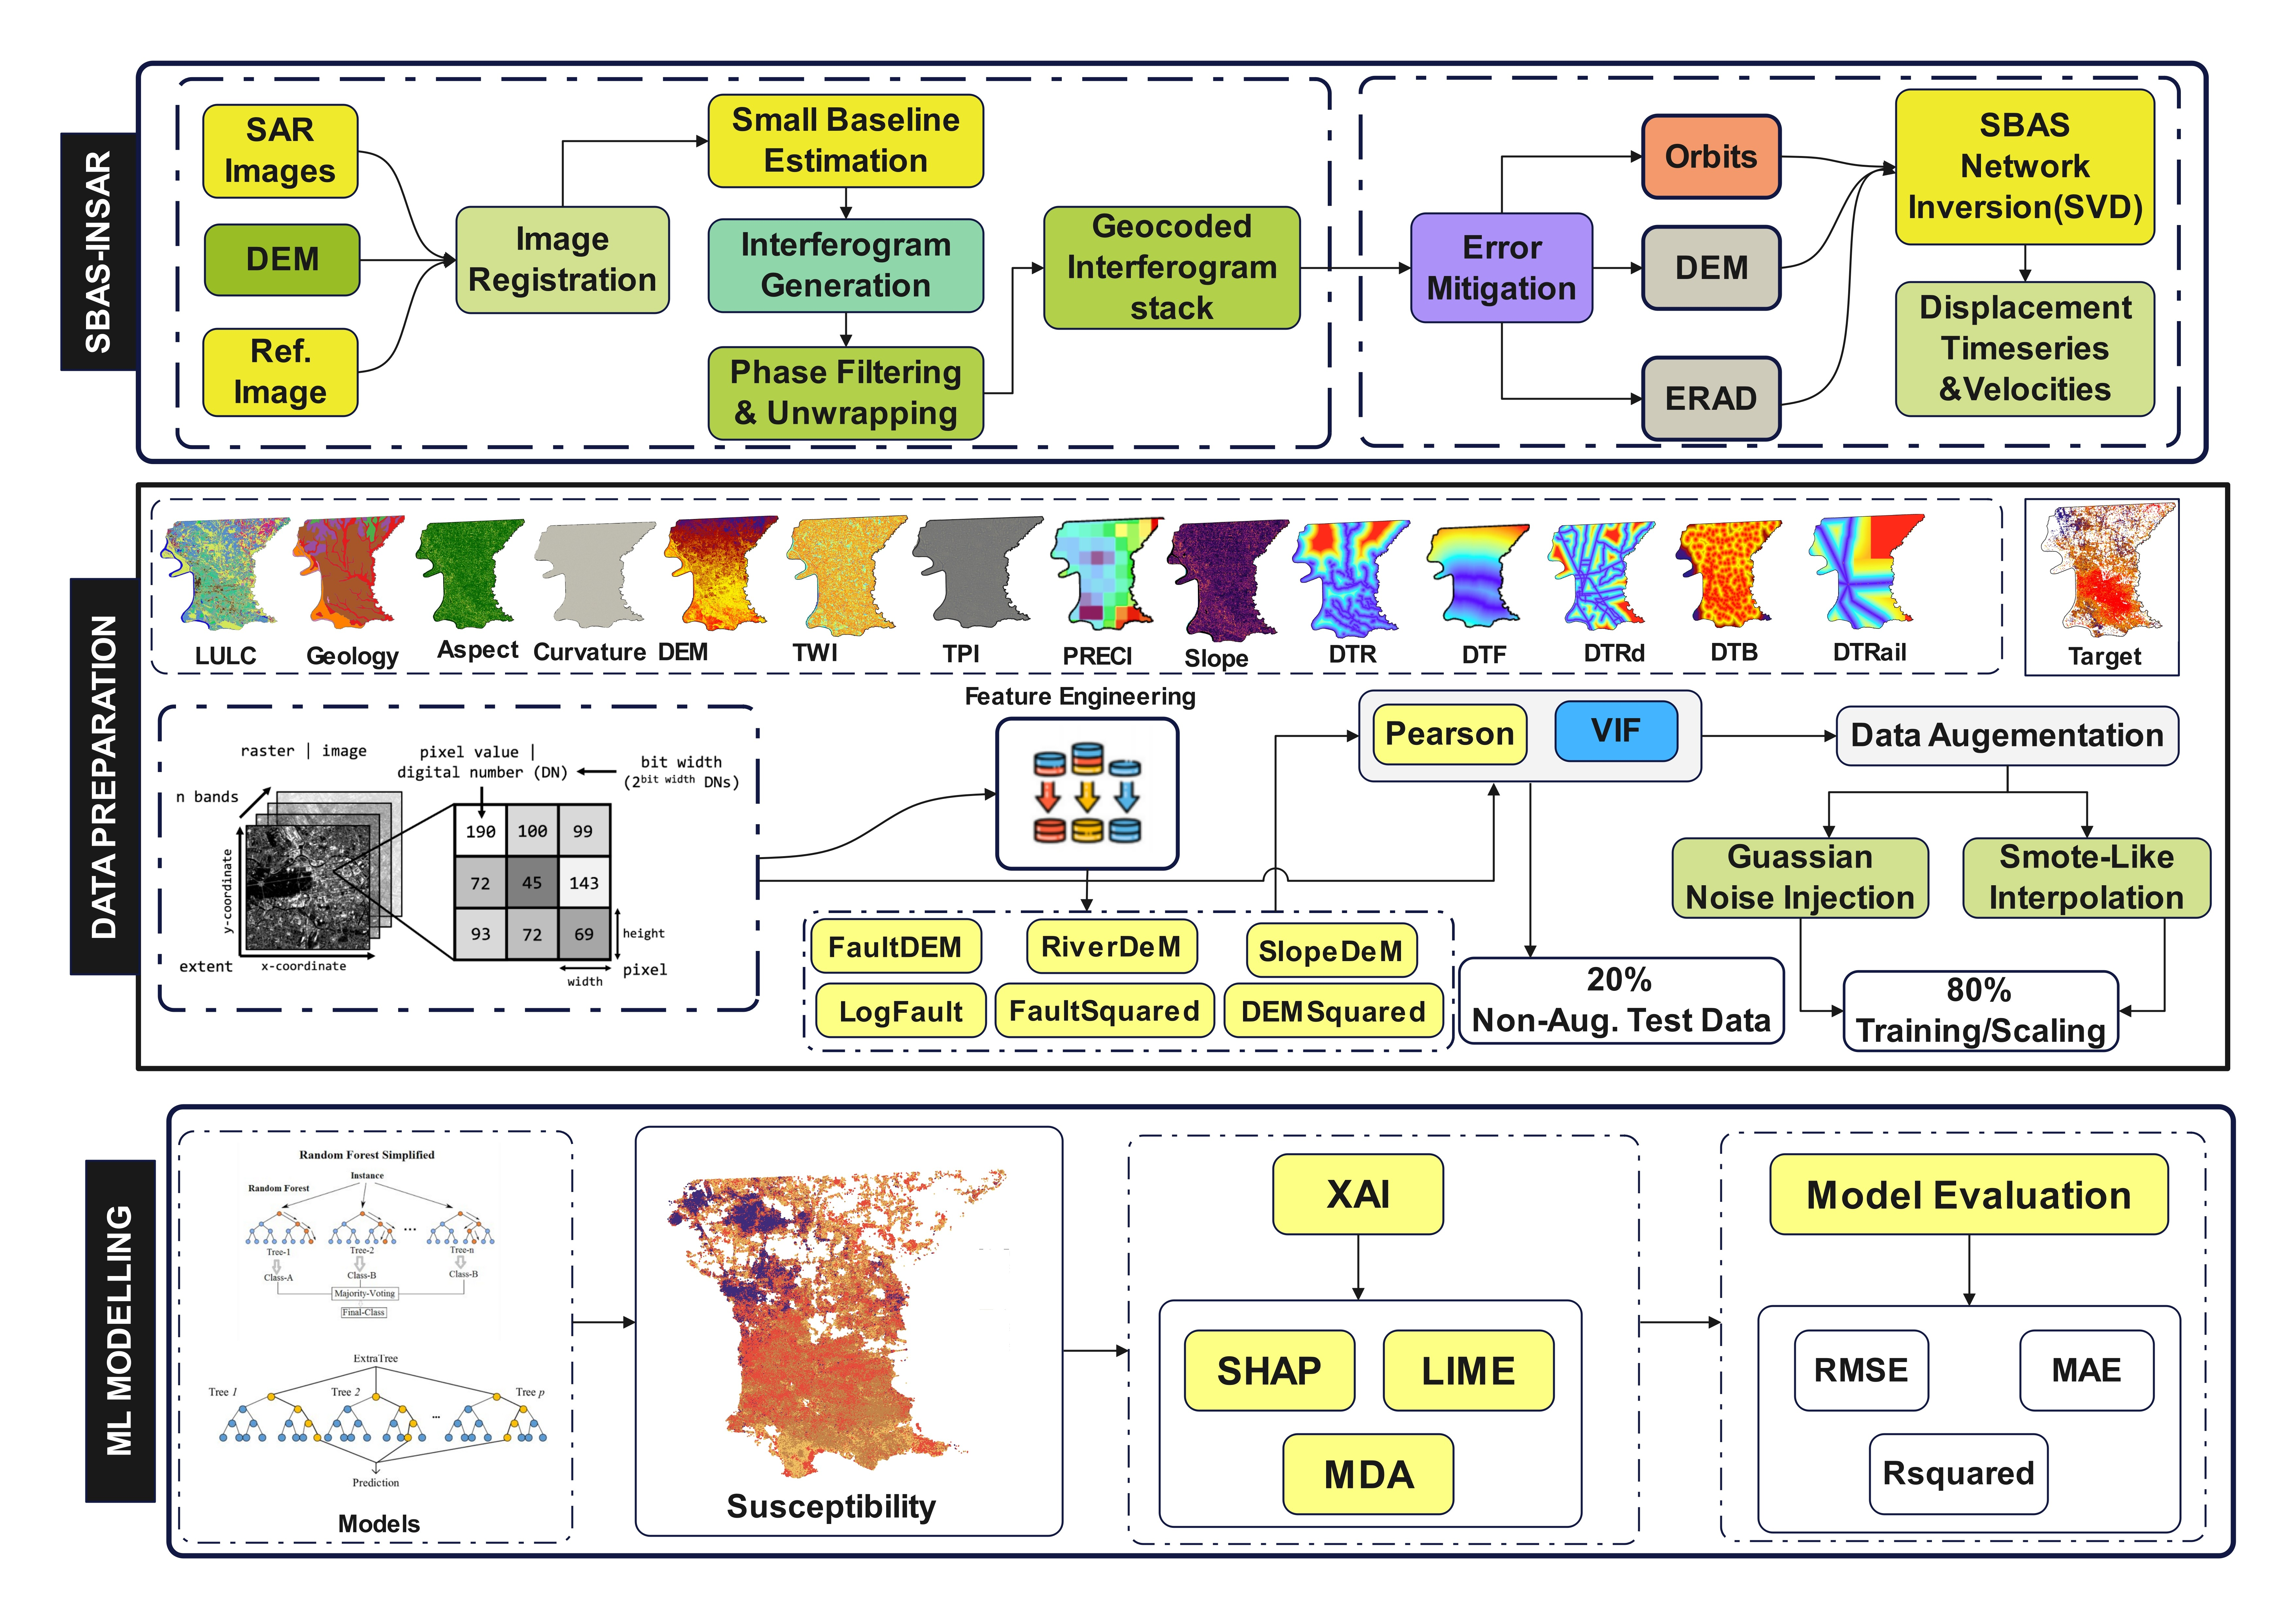
\includegraphics[width=0.95\textwidth,keepaspectratio]{Flowchart.jpg}
\caption{Susceptibility prediction flowchart}
\label{fig:methodology_flowchart}
\end{figure}

For the $i$-th differential interferogram constructed within the temporal interval between acquisitions $t_A$ and $t_B$, the phase corresponding to any pixel within the interferogram can be formulated as:
\begin{equation}
\begin{aligned}
\delta\phi_i(x,r) &= \phi(t_B, x, r) - \phi(t_A, x, r) \\
&\approx \frac{4\pi}{\lambda}[d(t_B, x, r) - d(t_A, x, r)] + \Delta\phi_{topo}(x,r) \\
&\quad + \Delta\phi_{atm}(x,r) + \Delta\phi_{noise}(x,r)
\end{aligned}
\end{equation}

In this formulation, $\phi(t_A, x, r)$ and $\phi(t_B, x, r)$ denote the phase values at spatial coordinates $(x, r)$ corresponding to times $t_A$ and $t_B$, respectively. The term $\Delta\phi_{topo}(x,r)$ represents residual topographic phase in the differential interferogram, $\Delta\phi_{atm}(x,r)$ accounts for atmospheric delay phase contributions, and $\Delta\phi_{noise}(x,r)$ represents the decoherence noise phase component. When digital elevation model (DEM) data are available, the topographic phase can be simulated and removed to eliminate terrain-induced phase errors \citep{Fattahi2015}. The phase matrix of all differential interferograms is denoted as $\delta\phi$, while the average surface deformation rate is represented by matrix $V$. The relationship between these matrices is expressed as:
\begin{equation}
BV = \delta\phi
\end{equation}

The dimensions of matrix $B$ are determined by $M$ and $N$. In general, matrix $B$ exhibits rank deficiency. Singular Value Decomposition (SVD) is conventionally applied for rank-deficient problem solving. Consequently, the acquisition of surface deformation information in time-series is achieved through the joint solution of multiple baseline sets, employing SVD to obtain the least-squares norm solution \citep{Berardino2002}.

The SBAS-InSAR processing was implemented using the 246 descending-track Sentinel-1 SLC acquisitions spanning 2017--2025. Perpendicular baseline thresholds were set to 150 m and temporal baselines to 48 days to maximize interferometric coherence while ensuring sufficient temporal sampling. Atmospheric phase delays were corrected using GACOS tropospheric delay models, and phase unwrapping was performed using the Minimum Cost Flow algorithm. The resulting velocity field was geocoded to a 30 m grid aligned with the conditioning factor layers for subsequent machine learning analysis.

\section{Environmental Conditioning Factors}
Fifteen geospatial conditioning factors were compiled at 30 m resolution to characterize the environmental and anthropogenic controls on subsidence, as illustrated in the methodology flowchart (Figure~\ref{fig:methodology_flowchart}) and detailed in Section 2.2.4 (Figures~\ref{fig:topo_factors}--\ref{fig:anthro_factors}). These factors span topographic attributes (DEM, slope, aspect, TPI, curvature, TWI), geological characteristics (geology, LULC), hydrological proximity (distance to rivers), structural controls (distance to faults), infrastructure proximity (distances to roads, railways, bridges), climatic variables (precipitation), and anthropogenic activity (interpolated groundwater well influence). Continuous variables were normalized using min-max scaling to [0,1], while categorical variables (geology, LULC) were one-hot encoded. The SBAS-derived velocity values at each 30 m pixel served as the target variable for supervised learning.

\section{Feature Engineering and Variable Transformation}
Feature engineering was conducted to enhance the predictive capability of the machine learning models by incorporating domain knowledge and enabling the representation of nonlinear and interaction effects among conditioning factors. This process aimed to improve model interpretability, stability, and generalization performance.

\subsection{Interaction Feature Construction}
Several interaction variables were generated to represent the combined influence of topographic, geological, and hydrological parameters on land displacement processes. Interaction features allow machine learning models to capture complex dependencies that cannot be represented using original variables alone \citep{Kuhn2019}. The following interaction terms were created:
\begin{equation}
\text{DTFDEM} = D_f \times E
\end{equation}
\begin{equation}
\text{DTRDEM} = D_r \times E
\end{equation}
\begin{equation}
\text{SlopeDEM} = S \times E
\end{equation}
where $D_f$ represents distance from geological faults, $D_r$ denotes distance from rivers, $E$ is elevation derived from the Digital Elevation Model (DEM), and $S$ is slope angle. These interaction variables represent how elevation modifies the influence of tectonic structures, drainage networks, and terrain steepness on surface deformation mechanisms.


\subsection{Polynomial Feature Generation}
To model nonlinear relationships between conditioning factors and displacement velocity, second-order polynomial features were introduced. Polynomial expansion enables machine learning models to better approximate curved response patterns and threshold effects \citep{Hastie2009}. The following squared variables were computed:
\begin{equation}
\text{DTF2} = D_f^2
\end{equation}
\begin{equation}
\text{DEM2} = E^2
\end{equation}
These features allow the models to capture nonlinear amplification or attenuation effects associated with proximity to fault zones and elevation gradients.

\subsection{Logarithmic Transformation}
Certain distance-related variables exhibited positive skewness and heteroscedasticity. To reduce distributional asymmetry and stabilize variance, logarithmic transformation was applied \citep{Osborne2010}. The transformed variable was calculated as:
\begin{equation}
\text{logDTF} = \ln(D_f + 1)
\end{equation}
where the constant 1 prevents undefined values when $D_f = 0$. Logarithmic scaling compresses extreme values and enhances model sensitivity to small-scale variations in fault-proximal regions.

\subsection{Assessment of Multicollinearity}
The introduction of interaction and polynomial features increased the potential risk of multicollinearity among predictors. Therefore, Variance Inflation Factor (VIF) analysis was performed to quantify interdependencies between variables \citep{Kutner2005}. VIF for each predictor was computed as:
\begin{equation}
\text{VIF}_i = \frac{1}{1 - R_i^2}
\end{equation}
where $R_i^2$ represents the coefficient of determination obtained by regressing the $i$-th variable against all remaining predictors. Although several engineered variables exhibited high VIF values, they were retained in the analysis because ensemble tree-based models are relatively insensitive to multicollinearity and can effectively exploit correlated predictors \citep{Dormann2013}.

\section{Data Augmentation}
To enhance model robustness, mitigate overfitting tendencies, and improve generalization capacity under conditions of measurement noise and sampling variability, data augmentation strategies were implemented to synthetically expand the training dataset, as illustrated in the methodology flowchart (Figure~\ref{fig:methodology_flowchart}). Augmentation introduces controlled perturbations into the original data, allowing machine learning algorithms to learn more comprehensive feature distributions and achieve greater predictive stability \citep{Shorten2019}. Given the inherent constraints in obtaining extensive, high-quality geospatial displacement measurements, augmentation was essential for strengthening the learning capacity of ensemble models.

\subsection{Gaussian Noise Injection}
Gaussian noise perturbation was applied to continuous predictor variables to simulate realistic measurement uncertainty and environmental stochasticity. This technique strengthens model robustness by training the algorithm on perturbed representations of the input feature space \citep{Bishop1995}. For each numerical feature $x_i$, augmented values were generated according to:
\begin{equation}
x_i^{\text{aug}} = x_i + \epsilon
\end{equation}
where the additive noise term $\epsilon$ is sampled from a Gaussian distribution:
\begin{equation}
\epsilon \sim \mathcal{N}(0, \sigma_i^2)
\end{equation}
with variance defined as:
\begin{equation}
\sigma_i = 0.02 \times \text{std}(x_i)
\end{equation}
Here, $\mathcal{N}(0, \sigma_i^2)$ represents a normal distribution with zero mean and variance $\sigma_i^2$, $\text{std}(x_i)$ denotes the standard deviation of feature $x_i$, and the coefficient 0.02 controls the magnitude of noise injection. Similarly, noise was introduced to the target variable:
\begin{equation}
y^{\text{aug}} = y + \eta, \quad \eta \sim \mathcal{N}(0, \sigma_y^2)
\end{equation}
where $\sigma_y = 0.02 \times \text{std}(y)$. This procedure maintains the underlying statistical structure of the dataset while incorporating realistic perturbations.

\subsection{Interpolation-Based Synthetic Sample Generation}
In addition to noise perturbation, synthetic samples were created using an interpolation technique adapted from the Synthetic Minority Over-sampling Technique (SMOTE) \citep{Chawla2002}. While SMOTE was originally formulated for classification tasks, this study adapted the approach for regression modeling. Two random samples $\mathbf{x}_a$ and $\mathbf{x}_b$ were selected from the original dataset, and new synthetic samples were generated through linear interpolation:
\begin{equation}
\mathbf{x}^{\text{syn}} = \alpha \mathbf{x}_a + (1 - \alpha)\mathbf{x}_b
\end{equation}
\begin{equation}
y^{\text{syn}} = \alpha y_a + (1 - \alpha)y_b
\end{equation}
where $\alpha \sim U(0.4, 0.6)$, with $U$ denoting a uniform distribution. This formulation ensures that synthetic samples are generated in the vicinity of existing observations, thereby avoiding unrealistic extrapolation. For categorical variables such as land-use class and geological type, values were inherited from a single parent sample:
\begin{equation}
x_j^{\text{syn}} = x_{a,j}, \quad \text{for categorical } x_j
\end{equation}
This approach preserves semantic consistency within the augmented dataset.

\subsection{Construction of the Augmented Dataset}
The final augmented dataset was assembled by concatenating the original dataset $D_{\text{orig}}$, the noise-augmented dataset $D_{\text{noise}}$, and the interpolated synthetic dataset $D_{\text{syn}}$. Formally:
\begin{equation}
D_{\text{aug}} = D_{\text{orig}} \cup D_{\text{noise}} \cup D_{\text{syn}}
\end{equation}
The resulting dataset size increased by approximately 2.5 times relative to the original, yielding a more comprehensive representation of the feature space and a total of 393,412 training samples.


To ensure unbiased model evaluation and prevent optimistic performance estimates, augmented samples were strictly confined to the training set, while only original samples were used for testing \citep{Kaufman2012}. Let $D_{\text{orig}} = D_{\text{train}}^{\text{orig}} \cup D_{\text{test}}$ and $D_{\text{aug}} = D_{\text{train}}^{\text{orig}} \cup D_{\text{noise}} \cup D_{\text{syn}}$. Thus:
\begin{equation}
D_{\text{train}} = D_{\text{train}}^{\text{orig}} \cup D_{\text{noise}} \cup D_{\text{syn}}
\end{equation}
\begin{equation}
D_{\text{test}} = D_{\text{test}}
\end{equation}
This strategy prevents artificially similar samples from appearing in both training and testing partitions, which would otherwise artificially inflate performance metrics.

\section{Extra Trees Algorithm}
This study employs both Random Forest and Extra Trees to determine which ensemble method provides optimal performance for subsidence susceptibility analysis, as outlined in the methodology flowchart (Figure~\ref{fig:methodology_flowchart}). Although RF is commonly used for geohazard applications, emerging evidence indicates that Extra Trees can deliver improved generalization performance when dealing with complex systems influenced by multiple factors \citep{Geurts2006}.

Extra Trees (ET) represents an ensemble technique that builds upon the Random Forest methodology. Two key differences distinguish ET from RF: (1) ET generates decision trees using randomly sampled subsets without replacement, which minimizes sampling bias, and (2) in ET, randomness is introduced through random threshold selection at splits rather than through bootstrap sampling \citep{Geurts2006}.
The splitting behavior in the ET framework is controlled by two key hyperparameters: $k$, which specifies how many features are randomly chosen at each node, and $n_{min}$, which defines the smallest permissible sample size for splitting a node. These parameters improve the model's ability to generalize and reduce the risk of overfitting \citep{Geurts2006}. The model structure is illustrated in Figure \ref{fig:etc_model}.


\begin{figure}[htbp]
\centering
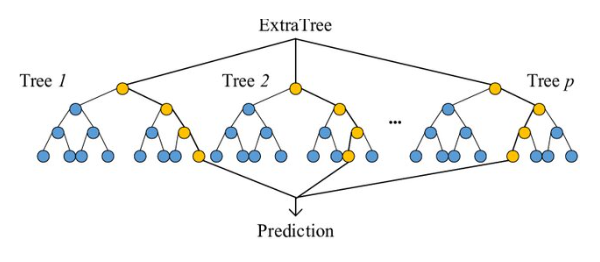
\includegraphics[width=0.6\textwidth]{ETC.png}
\caption{Extra Trees model architecture}
\label{fig:etc_model}
\end{figure}

Similar to RF, the ET method performs regression in two distinct stages: bootstrap sampling followed by aggregation. In the bootstrap stage, random subsets of training data are extracted to build individual trees. During aggregation, node splits are performed using randomly chosen feature subsets. The ensemble prediction is obtained by averaging outputs across all trees constructed from these random subsets. The mathematical representation of ET regression is given by \citet{Breiman2001}:
\begin{equation}
p(x, \beta_1, \ldots, \beta_n) = \frac{1}{m} \sum_{i=1}^{m} p(x, \beta_n)
\end{equation}
where $p$ denotes the prediction from the $p$-th tree, and $\beta$ represents a random vector governing tree construction.

\section{Random Forest Model}
RF is a supervised machine-learning algorithm that uses several decision trees to produce predictions that are more precise. RF is an ensemble learning technique that produces the mean prediction for regression tasks by combining the predictions of several decision tree models (Figure~\ref{fig:rf_model}) \citep{Breiman2001,wahba2024forecasting}.
The RF regressor operates an estimator that fits a collection of N randomized decision tree regressors independently and identically distributes random vectors \citep{Breiman2001}.

\begin{figure}[htbp]
\centering
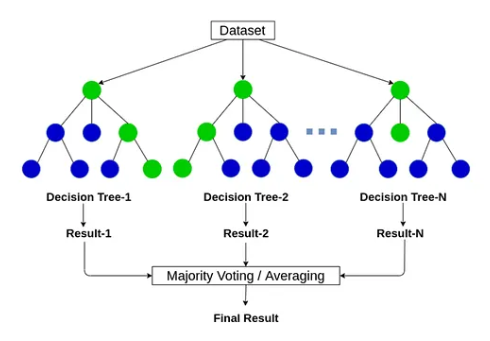
\includegraphics[width=0.6\textwidth]{RF_Figure.png}
\caption{Random Forest model architecture}
\label{fig:rf_model}

\end{figure}

The RF training procedure begins by generating random subsets from the original training dataset consisting of independently and identically distributed $[0, 1]^d \times \mathbb{R}$-valued random variables ($d \geq 2$) with comparable distribution properties to the independent generic pairs $(x, y)$. This is achieved by randomly resampling a specified proportion of the complete dataset $t_n = \{(x_1, y_1), \ldots, (x_n, y_n)\}$.
 This bootstrap aggregating (bagging) technique constructs multiple unpruned decision trees (DTs) \citep{Breiman2017CART, Breiman1996Bagging}. Subsequently, $K$ input features are randomly selected for splitting at each node during the training of individual decision trees. The prediction output from the $n$-th decision tree is represented as $g(x, t_N^n)$, and the aggregate prediction obtained by averaging across all constituent trees forms the final forest predictor, expressed in Equation~(5):
\begin{equation}
\hat{y} = \frac{1}{n} \sum_{i=1}^{n} g(x, t_m^n)
\end{equation}
where $\hat{y}$ represents the final prediction of the Random Forest model.

\section{Feature Importance and Model Explainability}
The inherent black-box nature of ensemble machine learning models, despite their superior predictive performance, presents significant challenges for interpretability in scientific applications. To address this limitation and enhance understanding of the decision-making processes underlying subsidence predictions, this study employs three complementary explainability techniques: SHAP, LIME, and MDI. These methods collectively provide both global and local interpretations of model behavior, feature importance, and individual prediction rationales \citep{Lundberg2017,yu_explainable_2025}.



\subsection{MDI}
MDI serves as a tree-based feature importance measure that quantifies the total reduction in node impurity attributable to splits on each feature, averaged across all trees in the ensemble \citep{Breiman2001}. For tree-based models such as RF and ET, MDI is computed during training by accumulating the weighted impurity decrease for each feature at every node where it is used for splitting. Mathematically, the importance $I_j$ of feature $j$ is expressed as:
\begin{equation}
I_j = \frac{1}{T} \sum_{t=1}^{T} \sum_{k \in S_t(j)} w_k \Delta i_k
\end{equation}
where $T$ denotes the total number of trees, $S_t(j)$ represents the set of splitting nodes using feature $j$ in tree $t$, $w_k$ is the weighted number of samples reaching node $k$, and $\Delta i_k$ is the impurity decrease at node $k$. Higher MDI values indicate features that contribute more substantially to reducing prediction uncertainty across the ensemble \citep{Cutler2007}.

\subsection{SHAP}
SHAP provides a unified framework for interpreting model predictions by assigning each feature an importance value for individual predictions, grounded in cooperative game theory \citep{Lundberg2017}. Unlike aggregate importance measures, SHAP values decompose each prediction into additive contributions from input features, satisfying desirable properties including local accuracy, missingness, and consistency \citep{yu_explainable_2025}. The SHAP value $\phi_j$ for feature $j$ quantifies its marginal contribution across all possible feature coalitions:
\begin{equation}
\phi_j = \sum_{S \subseteq F \setminus \{j\}} \frac{|S|!(|F|-|S|-1)!}{|F|!} \left[f(S \cup \{j\}) - f(S)\right]
\end{equation}
where $F$ represents the complete feature set, $S$ denotes a subset excluding feature $j$, $f(S)$ is the model prediction using only features in $S$, and $|\cdot|$ denotes set cardinality. For tree-based models, TreeSHAP algorithm enables efficient exact computation by exploiting the tree structure, avoiding exponential computational complexity \citep{Lundberg2017}.

SHAP values offer several analytical advantages. First, they provide instance-level explanations, revealing how individual features influence specific predictions. Second, aggregated SHAP values yield global feature importance rankings. Third, dependence plots visualize feature effects across their value ranges, exposing non-linear relationships and interaction effects. Fourth, SHAP values maintain consistency: if a model changes such that a feature's contribution increases, its SHAP value reflects this change proportionally \citep{yu_explainable_2025}.

\subsection{LIME}
LIME generates interpretable explanations for individual predictions by approximating the complex model locally with a simpler, interpretable surrogate model \citep{Ribeiro2016}. The technique operates by perturbing the input instance, obtaining predictions for perturbed samples, and fitting a linear model weighted by proximity to the original instance. For a prediction $f(x)$ at instance $x$, LIME solves the optimization problem:
\begin{equation}
\xi(x) = \arg\min_{g \in G} \mathcal{L}(f, g, \pi_x) + \Omega(g)
\end{equation}
where $G$ represents the class of interpretable models (typically linear models), $\mathcal{L}$ measures the fidelity of surrogate model $g$ in approximating $f$ within the local region defined by proximity kernel $\pi_x$, and $\Omega(g)$ penalizes model complexity to ensure interpretability.

The LIME procedure generates $N$ perturbed samples in the neighborhood of $x$, obtains their predictions from the original model, and weights them according to their proximity to $x$ using an exponential kernel. The resulting linear approximation identifies which features contribute most significantly to the specific prediction, providing locally faithful explanations even when global model behavior is highly non-linear.

\subsection{Integrated Explainability Framework}
This study employs these three methods synergistically to achieve comprehensive model interpretability. MDI provides computationally efficient global feature rankings inherent to the tree ensemble structure. SHAP analysis delivers theoretically grounded feature attributions with both local (instance-level) and global (aggregated) interpretability, enabling identification of dominant subsidence drivers and their directional effects. LIME complements these approaches by offering human-interpretable local explanations that validate SHAP findings and provide intuitive justifications for individual high-risk predictions.

By triangulating results across these explainability techniques, this framework addresses critical limitations of black-box models in geohazard assessment, transforming predictive models into decision-support tools that provide not only accurate forecasts but also scientifically interpretable explanations of subsidence mechanisms \citep{yu_explainable_2025,Pradhan2023}. This integrated approach enables stakeholders to understand which environmental and anthropogenic factors drive subsidence risk in specific locations, facilitating targeted mitigation strategies and informed land-use planning decisions.

\section{Physics-Informed LSTM for Spatio-Temporal Forecasting}
While tree-based ensemble models excel at spatial susceptibility mapping by capturing complex relationships between environmental factors and subsidence patterns, they do not explicitly model temporal dependencies inherent in time-series deformation data. To address this limitation and enable robust near-decadal subsidence forecasting, this study implements a hybrid framework that integrates Bidirectional Long Short-Term Memory (Bi-LSTM) neural networks with physics-informed constraints (Figure~\ref{fig:lstm_forecast_flowchart}). This approach combines data-driven learning of spatio-temporal patterns from InSAR time series with geomechanically consistent rules that ensure physically plausible long-term projections.

\begin{figure}[!t]
\centering

\includegraphics[width=0.95\textwidth,keepaspectratio]{master_thesis_forcast.jpg.jpeg}
\caption{Physics-informed Bi-LSTM forecasting framework}
\label{fig:lstm_forecast_flowchart}
\end{figure}

\subsection{Framework Overview and Conceptual Rationale}
The physics-informed forecasting framework (Figure~\ref{fig:lstm_forecast_flowchart}) operates in two distinct stages: (1) a prediction stage, where a Bi-LSTM model is trained to learn subsidence dynamics from historical SBAS-InSAR observations, and (2) a forecasting stage, where the trained network is iteratively applied in autoregressive mode with physics-based constraints to ensure temporal stability and geomechanical realism during extrapolation beyond the observation period \citep{Raissi2019,Zhu2024}. This separation ensures that machine learning captures complex non-linear variability in the training data, while physical principles govern long-term behavior to prevent unrealistic acceleration, deceleration, or sign reversal commonly observed in purely data-driven extrapolation.

Unlike Physics-Informed Neural Networks (PINNs) that encode partial differential equations directly into the loss function during training, the present approach applies constraints post-prediction during the autoregressive forecasting loop \citep{Raissi2019}. This design choice maintains model flexibility during training while ensuring physical consistency during deployment, thereby balancing predictive accuracy with geomechanical plausibility.


\subsection{Data Preprocessing and Input Construction}
As illustrated in Figure~\ref{fig:lstm_forecast_flowchart}, to suppress atmospheric noise and low-signal artifacts in the SBAS-InSAR time series, only pixels exhibiting absolute mean velocity exceeding a significance threshold were retained for temporal modeling:
\begin{equation}
|v| \geq 1.5 \ \text{mm yr}^{-1}
\end{equation}
where $v$ represents the mean annual subsidence velocity. This threshold reduces contributions from decorrelated or atmospherically contaminated pixels while preserving meaningful deformation signals.

Each retained time series was normalized using min--max scaling to stabilize gradient propagation during neural network training:
\begin{equation}
x_t^{*} = \frac{x_t - x_{\min}}{x_{\max} - x_{\min}}
\end{equation}
where $x_t$ denotes the observed subsidence velocity at time $t$, and $x_{\min}$ and $x_{\max}$ represent the minimum and maximum values across the entire time series.


A supervised learning structure was constructed using a sliding window approach to generate input-output pairs for sequential prediction. The input window length was set to 18 months to capture seasonal and interannual variability, while the output window was set to 6 months to enable multi-step-ahead forecasting. Formally, for a time series $\{x_t\}_{t=1}^{T}$, the input-output mapping at time index $i$ is defined as:
\begin{equation}
\mathbf{X}_i = [x_{t-17}, \dots, x_t], \quad \mathbf{Y}_i = [x_{t+1}, \dots, x_{t+6}]
\end{equation}
This formulation enables the network to learn temporal dependencies while supporting direct multi-horizon prediction, which is essential for operational forecasting applications.


\subsection{LSTM Architecture and Temporal Dependency Modeling}
LSTM networks address the vanishing gradient problem inherent in traditional recurrent neural networks by introducing gated memory cells that selectively retain or discard information across long sequences \citep{Hochreiter1997}. Each LSTM cell maintains a cell state $C_t$ and a hidden state $h_t$, governed by three gating mechanisms: the forget gate $f_t$, input gate $i_t$, and output gate $o_t$. The LSTM cell equations are formulated as:
\begin{equation}
f_t = \sigma(W_f [h_{t-1}, x_t] + b_f)
\end{equation}
\begin{equation}
i_t = \sigma(W_i [h_{t-1}, x_t] + b_i)
\end{equation}
\begin{equation}
\tilde{C}_t = \tanh(W_c [h_{t-1}, x_t] + b_c)
\end{equation}
\begin{equation}
C_t = f_t \odot C_{t-1} + i_t \odot \tilde{C}_t
\end{equation}
\begin{equation}
o_t = \sigma(W_o [h_{t-1}, x_t] + b_o)
\end{equation}
\begin{equation}
h_t = o_t \odot \tanh(C_t)
\end{equation}
where $\sigma(\cdot)$ denotes the sigmoid activation function, $\tanh(\cdot)$ is the hyperbolic tangent activation, $\odot$ represents element-wise multiplication, $W_f, W_i, W_c, W_o$ are weight matrices, and $b_f, b_i, b_c, b_o$ are bias vectors. The forget gate controls which information from the previous cell state is discarded, the input gate regulates new information incorporation, and the output gate determines the hidden state exposed to subsequent layers.

\subsection{Bidirectional LSTM Formulation}
Land subsidence time series exhibit both short-term fluctuations driven by seasonal hydrological cycles and long-term trends associated with aquifer compaction. Standard unidirectional LSTM processes sequences in forward temporal order, potentially missing contextual information from future time steps within the input window. Bidirectional LSTM addresses this limitation by processing the input sequence in both forward and backward directions, enabling the network to exploit complete temporal context \citep{Schuster1997}.

For each time step $t$ within the input window, the Bi-LSTM computes forward and backward hidden states:
\begin{equation}
\overrightarrow{h_t} = \text{LSTM}_{\text{forward}}(x_t, \overrightarrow{h_{t-1}})
\end{equation}
\begin{equation}
\overleftarrow{h_t} = \text{LSTM}_{\text{backward}}(x_t, \overleftarrow{h_{t+1}})
\end{equation}
The final hidden representation at time $t$ is obtained by concatenating the forward and backward states:
\begin{equation}
h_t = [\overrightarrow{h_t}, \overleftarrow{h_t}]
\end{equation}
This bidirectional processing captures both antecedent conditions and subsequent trends within the input window, improving the model's ability to distinguish persistent deformation from transient noise.

\subsection{Network Architecture and Training Configuration}
The adopted Bi-LSTM architecture (Figure~\ref{fig:lstm_forecast_flowchart}) consists of two stacked bidirectional layers with progressively decreasing dimensionality to extract hierarchical temporal features. The first Bi-LSTM layer contains 192 units (96 forward, 96 backward), followed by batch normalization and dropout regularization to prevent overfitting.


The model was trained using the Adam optimizer \citep{Kingma2014} with an initial learning rate of 0.001, which was reduced on plateau using a learning rate scheduler. The loss function is mean squared error (MSE) between predicted and observed velocity sequences:
\begin{equation}
\mathcal{L}_{\text{MSE}} = \frac{1}{N} \sum_{i=1}^{N} (y_i - \hat{y}_i)^2
\end{equation}
where $N$ is the total number of time steps, $y_i$ is the observed velocity, and $\hat{y}_i$ is the predicted velocity. Training was conducted exclusively on historical data without physics-based constraints, allowing the network to learn unconstrained temporal patterns. Physics-informed corrections are applied only during the forecasting stage.

\subsection{Autoregressive Forecasting Strategy}
After training, the Bi-LSTM is deployed in autoregressive forecasting mode to generate long-term subsidence projections (Figure~\ref{fig:lstm_forecast_flowchart}). The procedure operates as follows: (1) the final 18 months of observed data are provided as the initial input window, (2) the trained Bi-LSTM predicts the next time step, (3) the predicted value is appended to the input sequence, (4) the oldest value is removed to maintain the 18-month window length, and (5) the process repeats iteratively to generate forecasts extending to 2030.

\subsection{Physics-Informed Constraint Module}
The physics-informed module (Figure~\ref{fig:lstm_forecast_flowchart}) does not modify the Bi-LSTM architecture or training process. Instead, it constrains Bi-LSTM outputs during autoregressive forecasting to enforce physically plausible subsidence evolution. The constraint framework incorporates five complementary mechanisms: exponential decay, hybrid blending, temporal smoothing, rate-of-change limitation, and sign preservation.

\noindent\textit{Exponential Subsidence Decay Model.}

Long-term subsidence rates in aquifer systems are expected to stabilize as pore pressure equilibration and sediment consolidation approach steady-state conditions.
\begin{equation}
x_{t+1}^{\text{phys}} = x_t (1 - r)^{\Delta t}
\end{equation}
where $x_t$ is the subsidence velocity at time $t$, $r$ is the decay constant representing the fractional reduction in velocity per unit time, and $\Delta t$ is the time increment in years. The decay constant $r$ was calibrated to 0.004 yr$^{-1}$ based on historical deceleration trends observed in the SBAS-InSAR time series and regional aquifer compaction studies \citep{Higgins2016}.

\noindent\textit{Hybrid LSTM--Physics Blending.}

The physics-based velocity estimate is blended with the raw Bi-LSTM prediction using a weighted combination:
\begin{equation}
x_{t+1} = \alpha x_{t+1}^{\text{LSTM}} + (1 - \alpha) x_{t+1}^{\text{phys}}
\end{equation}
where $x_{t+1}^{\text{LSTM}}$ is the unconstrained Bi-LSTM output, $x_{t+1}^{\text{phys}}$ is the physics-based decay estimate, and $\alpha \in [0,1]$ is a blending coefficient. This formulation allows the LSTM to capture short-term variability and local deviations from idealized decay behavior, while physics governs long-term trends. The coefficient $\alpha$ was set to 0.65, prioritizing data-driven predictions in the near term while increasing the influence of physics-based stabilization in the far-future forecast horizon.

\noindent\textit{Temporal Continuity Constraint.}

To prevent abrupt temporal discontinuities that violate geomechanical principles, a temporal smoothing filter is applied:
\begin{equation}
x_{t+1}^{\text{smooth}} = \beta x_{t+1} + (1 - \beta) x_t
\end{equation}
where $\beta$ controls the degree of smoothing. Higher $\beta$ values preserve more of the predicted signal, while lower values enforce stronger temporal continuity. The parameter $\beta$ was set to 0.85 to balance responsiveness to predicted trends with suppression of unrealistic jumps.

\noindent\textit{Rate-of-Change Limitation.}

Physical limits on subsidence acceleration are enforced by constraining the maximum allowable velocity change between consecutive time steps:
\begin{equation}
|x_{t+1} - x_t| \leq \Delta_{\max}
\end{equation}
where $\Delta_{\max}$ is defined as a fraction of the previous velocity magnitude: $\Delta_{\max} = 0.15|x_t|$. This constraint prevents unphysical acceleration or deceleration that would correspond to instantaneous changes in aquifer stress conditions.

\noindent\textit{Sign Preservation.}

To prevent unphysical sign reversal, where subsiding regions spontaneously transition to uplift without corresponding groundwater recharge or tectonic forcing, the sign consistency constraint is applied:
\begin{equation}
\text{sign}(x_{t+1}) = \text{sign}(x_t)
\end{equation}
This ensures that the directional character of deformation is maintained throughout the forecast period, consistent with the persistent stress regime in East Baton Rouge Parish.


\noindent\textit{Stochastic Variability Representation.}


Small-magnitude Gaussian noise is added to represent unresolved spatiotemporal heterogeneity and measurement uncertainty:
\begin{equation}
x_{t+1}^{\text{final}} = x_{t+1} + \epsilon, \quad \epsilon \sim \mathcal{N}(0, \sigma^2)
\end{equation}
where $\sigma$ is set to 2\% of the current velocity magnitude. This stochastic component prevents over-deterministic forecasts and provides a mechanism for ensemble-based uncertainty quantification.

The proposed framework employs a Bi-LSTM network for data-driven prediction of subsidence time series and a physics-informed constraint module for long-term forecasting stabilization. The Bi-LSTM captures complex temporal patterns including seasonal fluctuations, interannual variability, and non-linear trends, while physical constraints enforce continuity, exponential decay, and directional stability during autoregressive forecasting. This hybrid approach yields realistic and robust near-decadal subsidence projections that balance empirical learning with geomechanical consistency, addressing a critical gap in subsidence forecasting methodologies \citep{Zhu2024,Mirmazloumi2023}.

\section{Model Performance Evaluation Metrics}
To ensure rigorous assessment of model performance across both spatial susceptibility mapping and temporal forecasting tasks, a comprehensive suite of quantitative metrics was employed. These metrics evaluate different aspects of model capability, including predictive accuracy, error magnitude, directional consistency, and distributional agreement between predicted and observed subsidence patterns. The evaluation framework is divided into regression metrics for continuous prediction assessment and correlation metrics for temporal pattern validation.

\subsection{Coefficient of Determination}
The coefficient of determination ($R^2$) quantifies the proportion of variance in the observed subsidence velocity explained by the model predictions \citep{Kutner2005}. It is computed as:
\begin{equation}
R^2 = 1 - \frac{\sum_{i=1}^{n}(y_i - \hat{y}_i)^2}{\sum_{i=1}^{n}(y_i - \bar{y})^2}
\end{equation}
where $y_i$ represents the $i$-th observed subsidence value, $\hat{y}_i$ is the corresponding model prediction, $\bar{y}$ denotes the mean of observed values, and $n$ is the total number of samples. $R^2$ values range from 0 to 1, with values approaching 1 indicating strong explanatory power. This metric serves as the primary indicator of model fit for both ET and RF susceptibility models, as well as the Bi-LSTM forecasting model.

\subsection{Root Mean Squared Error}
Root Mean Squared Error (RMSE) measures the average magnitude of prediction errors in the same units as the target variable, providing an interpretable assessment of absolute model accuracy \citep{Chai2014}. RMSE is calculated as:
\begin{equation}
\text{RMSE} = \sqrt{\frac{1}{n}\sum_{i=1}^{n}(y_i - \hat{y}_i)^2}
\end{equation}
RMSE penalizes larger errors more heavily than smaller ones due to the squaring operation, making it sensitive to outliers and large deviations. In the context of subsidence monitoring, RMSE quantifies typical prediction error in mm/yr for velocity predictions and mm for cumulative displacement forecasts.

\subsection{Mean Absolute Error}
Mean Absolute Error (MAE) provides a robust measure of average prediction error that is less sensitive to outliers compared to RMSE \citep{Willmott2005}:
\begin{equation}
\text{MAE} = \frac{1}{n}\sum_{i=1}^{n}|y_i - \hat{y}_i|
\end{equation}
MAE represents the average absolute deviation between predictions and observations without emphasizing extreme errors. The comparison between RMSE and MAE values provides insight into error distribution: when RMSE substantially exceeds MAE, it indicates the presence of large prediction errors or outliers that disproportionately influence model performance.

\subsection{Mean Absolute Percentage Error}
Mean Absolute Percentage Error (MAPE) expresses prediction error as a percentage of observed values, enabling scale-independent comparison across different magnitudes of subsidence \citep{Hyndman2006}:
\begin{equation}
\text{MAPE} = \frac{100\%}{n}\sum_{i=1}^{n}\left|\frac{y_i - \hat{y}_i}{y_i}\right|
\end{equation}
MAPE is particularly useful for evaluating forecast performance across spatial regions experiencing different subsidence rates. However, MAPE becomes undefined when observed values approach zero and can produce asymmetric error penalties. Therefore, MAPE is reported alongside absolute error metrics to provide complementary performance perspectives.

\subsection{Pearson Correlation Coefficient}
The Pearson correlation coefficient ($r$) quantifies the strength and direction of linear association between predicted and observed values \citep{Rodgers1988}:
\begin{equation}
r = \frac{\sum_{i=1}^{n}(y_i - \bar{y})(\hat{y}_i - \bar{\hat{y}})}{\sqrt{\sum_{i=1}^{n}(y_i - \bar{y})^2}\sqrt{\sum_{i=1}^{n}(\hat{y}_i - \bar{\hat{y}})^2}}
\end{equation}
where $\bar{\hat{y}}$ represents the mean of predicted values. Pearson correlation ranges from $-1$ to $+1$, with values near $+1$ indicating strong positive linear correspondence. Unlike $R^2$, which assesses goodness-of-fit, the Pearson coefficient evaluates whether predictions and observations co-vary proportionally, making it valuable for assessing temporal pattern replication in time-series forecasting.


\subsection{Nash-Sutcliffe Efficiency}
The Nash-Sutcliffe Efficiency (NSE) coefficient is widely used in hydrological and geophysical modeling to evaluate predictive skill relative to a baseline mean model \citep{Nash1970}:
\begin{equation}
\text{NSE} = 1 - \frac{\sum_{i=1}^{n}(y_i - \hat{y}_i)^2}{\sum_{i=1}^{n}(y_i - \bar{y})^2}
\end{equation}
NSE ranges from $-\infty$ to 1, where NSE = 1 indicates perfect prediction, NSE = 0 indicates performance equivalent to using the mean as a predictor, and NSE $<$ 0 indicates predictions worse than the mean. NSE is mathematically equivalent to $R^2$ for unbiased models but can differ when systematic bias exists. High NSE values confirm that model predictions outperform naive baseline approaches.

\subsection{Model Comparison and Selection Criteria}
For susceptibility mapping, model selection between ET and RF is based on test-set $R^2$, RMSE, and MAE computed on hold-out data not used during training or hyperparameter optimization. The optimal model demonstrates superior performance across multiple metrics while maintaining computational efficiency and interpretability. For temporal forecasting, the physics-informed Bi-LSTM is evaluated using $R^2$, RMSE, MAE, Pearson correlation, and NSE on validation time periods, with particular emphasis on forecast stability and absence of unphysical trends during long-term extrapolation. Additionally, comparison with GNSS vertical displacement measurements at 1LSU and GMVS stations provides independent ground-truth validation of InSAR-derived and model-predicted subsidence rates \citep{Abdalla2024}.

\clearpage
\chapter[Results and Discussion]{\centering Results and Discussion}

This chapter presents the integrated results of SBAS-InSAR deformation analysis, machine learning-based susceptibility mapping,
 explainable AI feature importance analysis, and physics-informed LSTM temporal forecasting for East Baton Rouge Parish.
The findings are discussed in relation to the geological, hydrological, and anthropogenic controls on subsidence processes.

\section{SBAS-InSAR Deformation Analysis}

The mean vertical displacement velocity across EBRP was $+0.46$~mm/yr, with a standard deviation of $\pm 3.98$~mm/yr,
indicating spatially heterogeneous ground deformation with both subsidence and uplift.
The SBAS-InSAR velocity map (Figure~\ref{fig:sbas_results}a) displays subsidence zones in red-orange and uplift areas in blue, 
with maximum subsidence rates of $-23.66$~mm/yr observed near fault systems and zones of intensive groundwater extraction with most in the 
southern urban corridor, while maximum uplift of $+19.18$~mm/yr occurred in elevated forested regions occuring in the 
northern parts of the parish. The derived SBAS susceptibility classification (Figure~\ref{fig:sbas_results}b) delineates high-risk zones (red), moderate-risk areas (yellow), and low-risk regions (green), reflecting complex interactions between geological, hydrological, and anthropogenic factors.

\begin{figure}[htbp]
\centering
\begin{tabular}{cc}
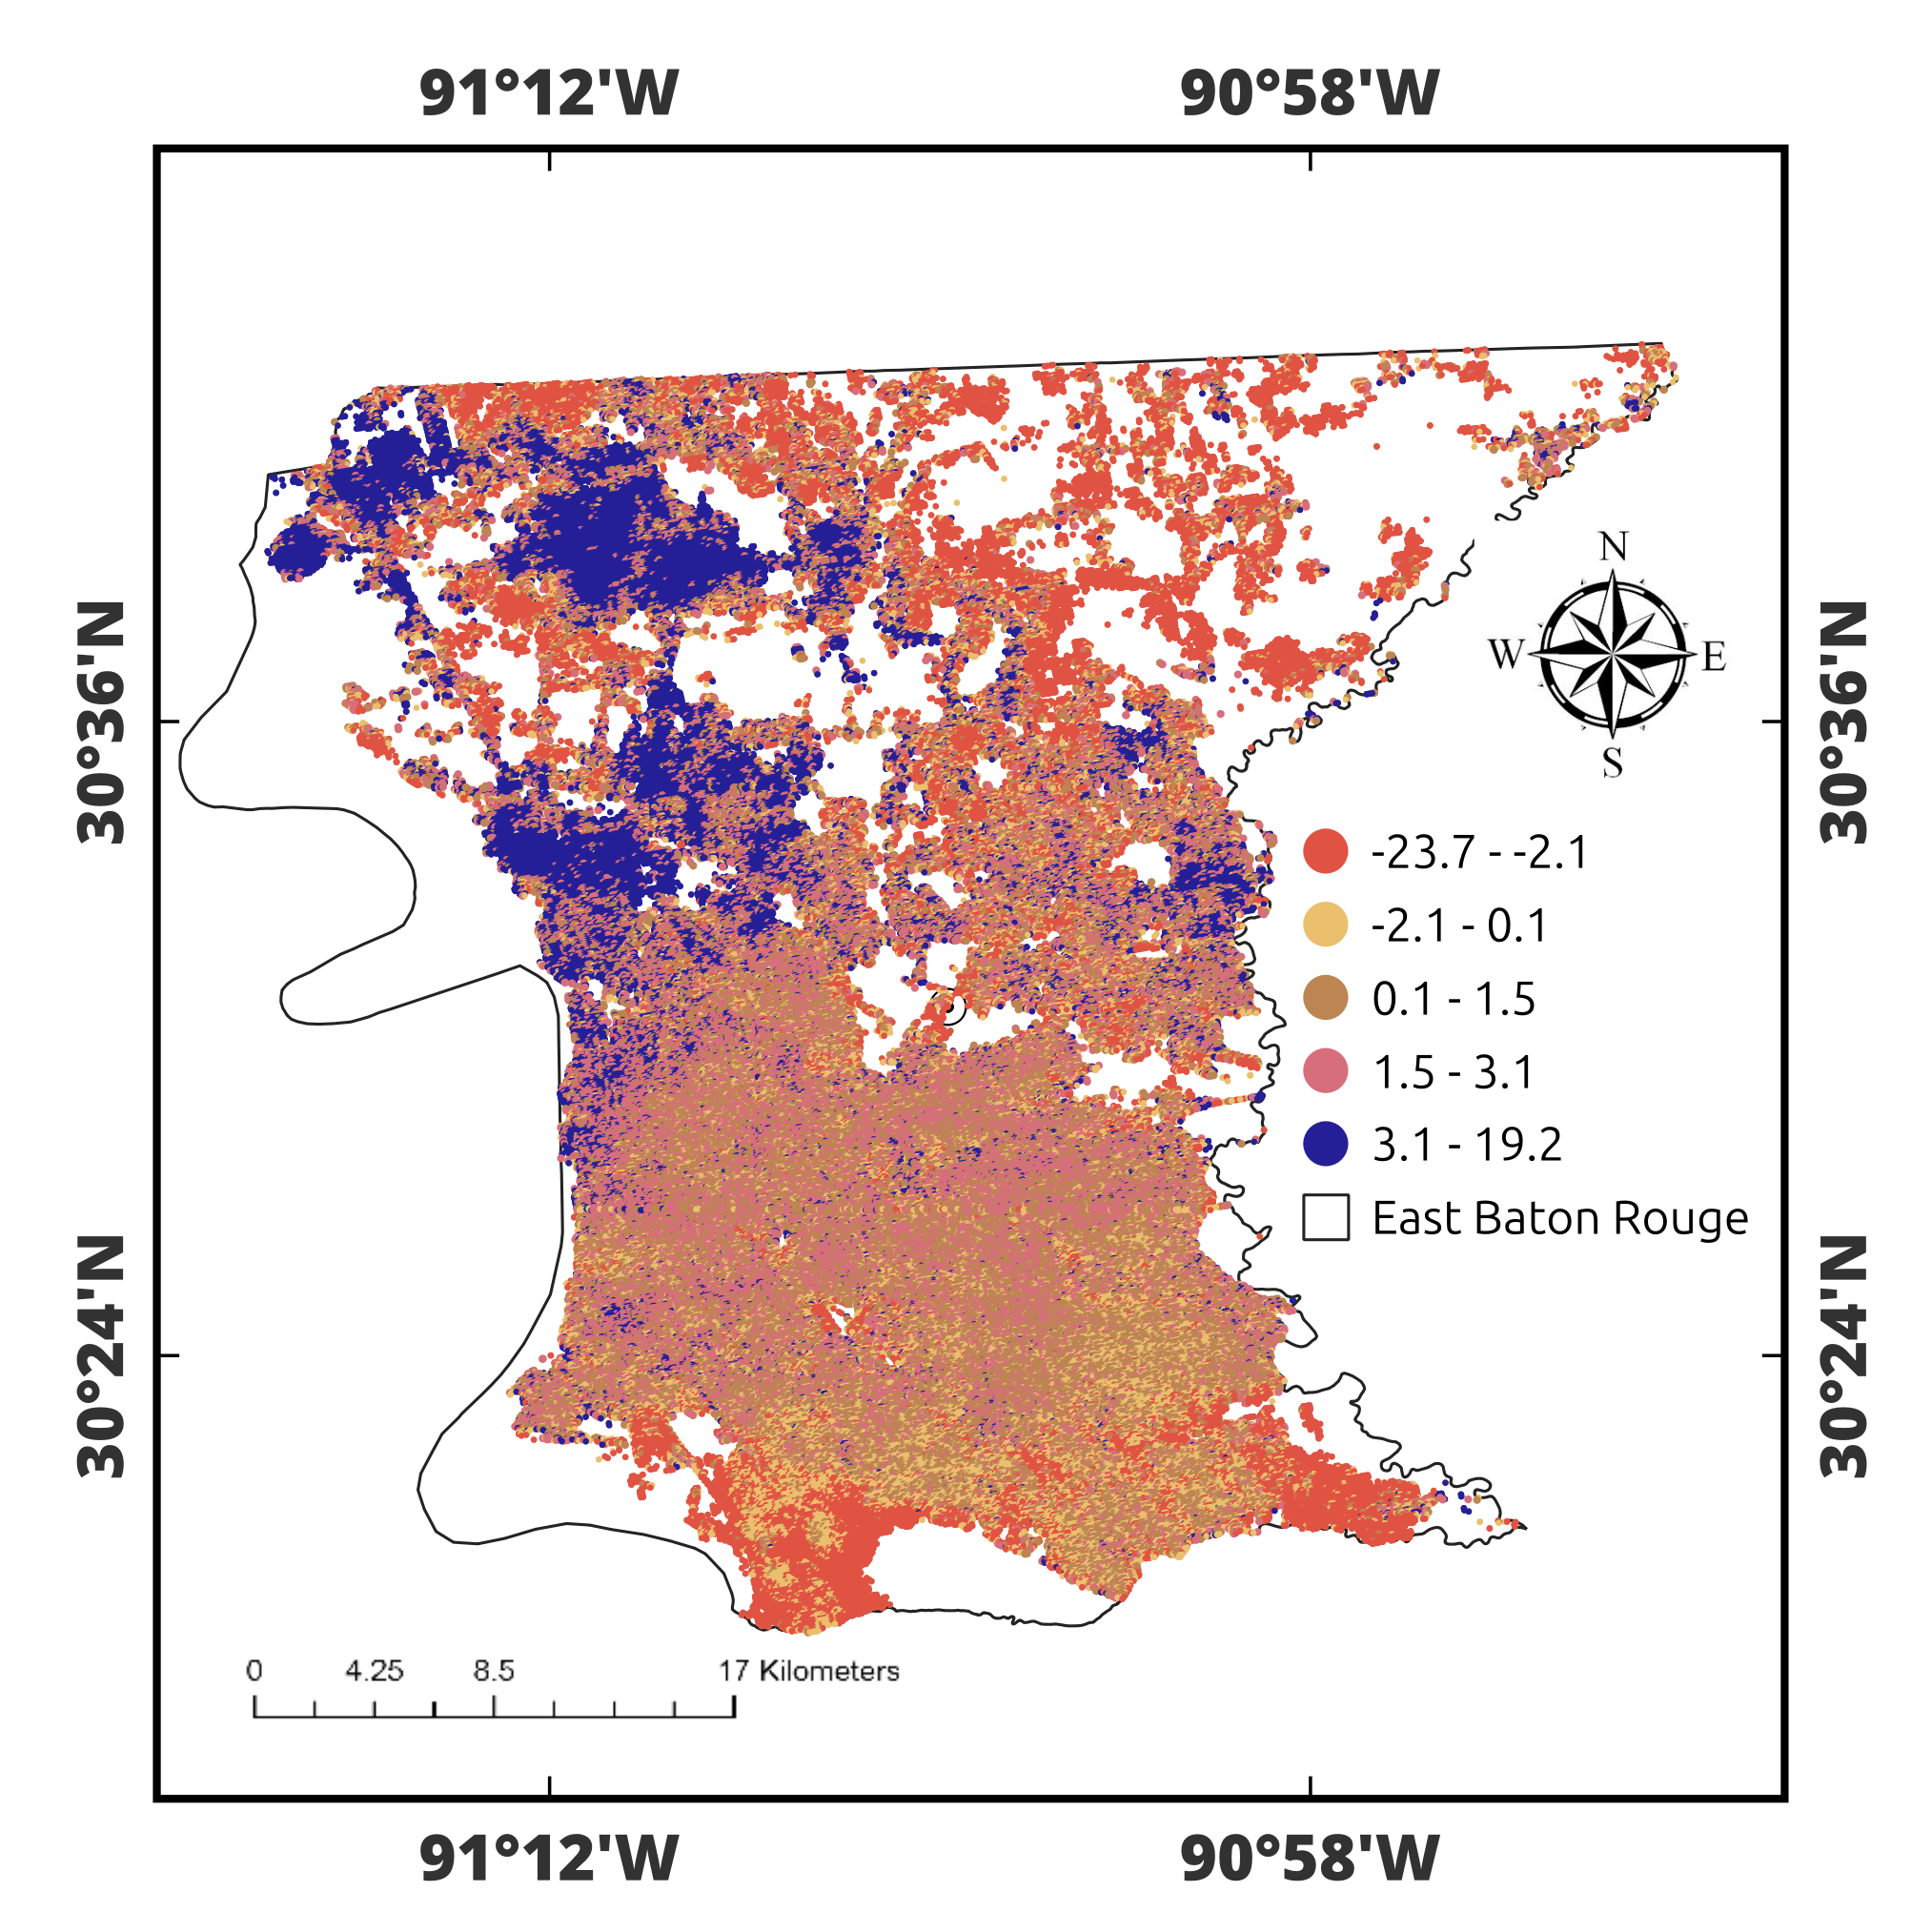
\includegraphics[width=0.48\textwidth]{media/sbas_vel.png} &
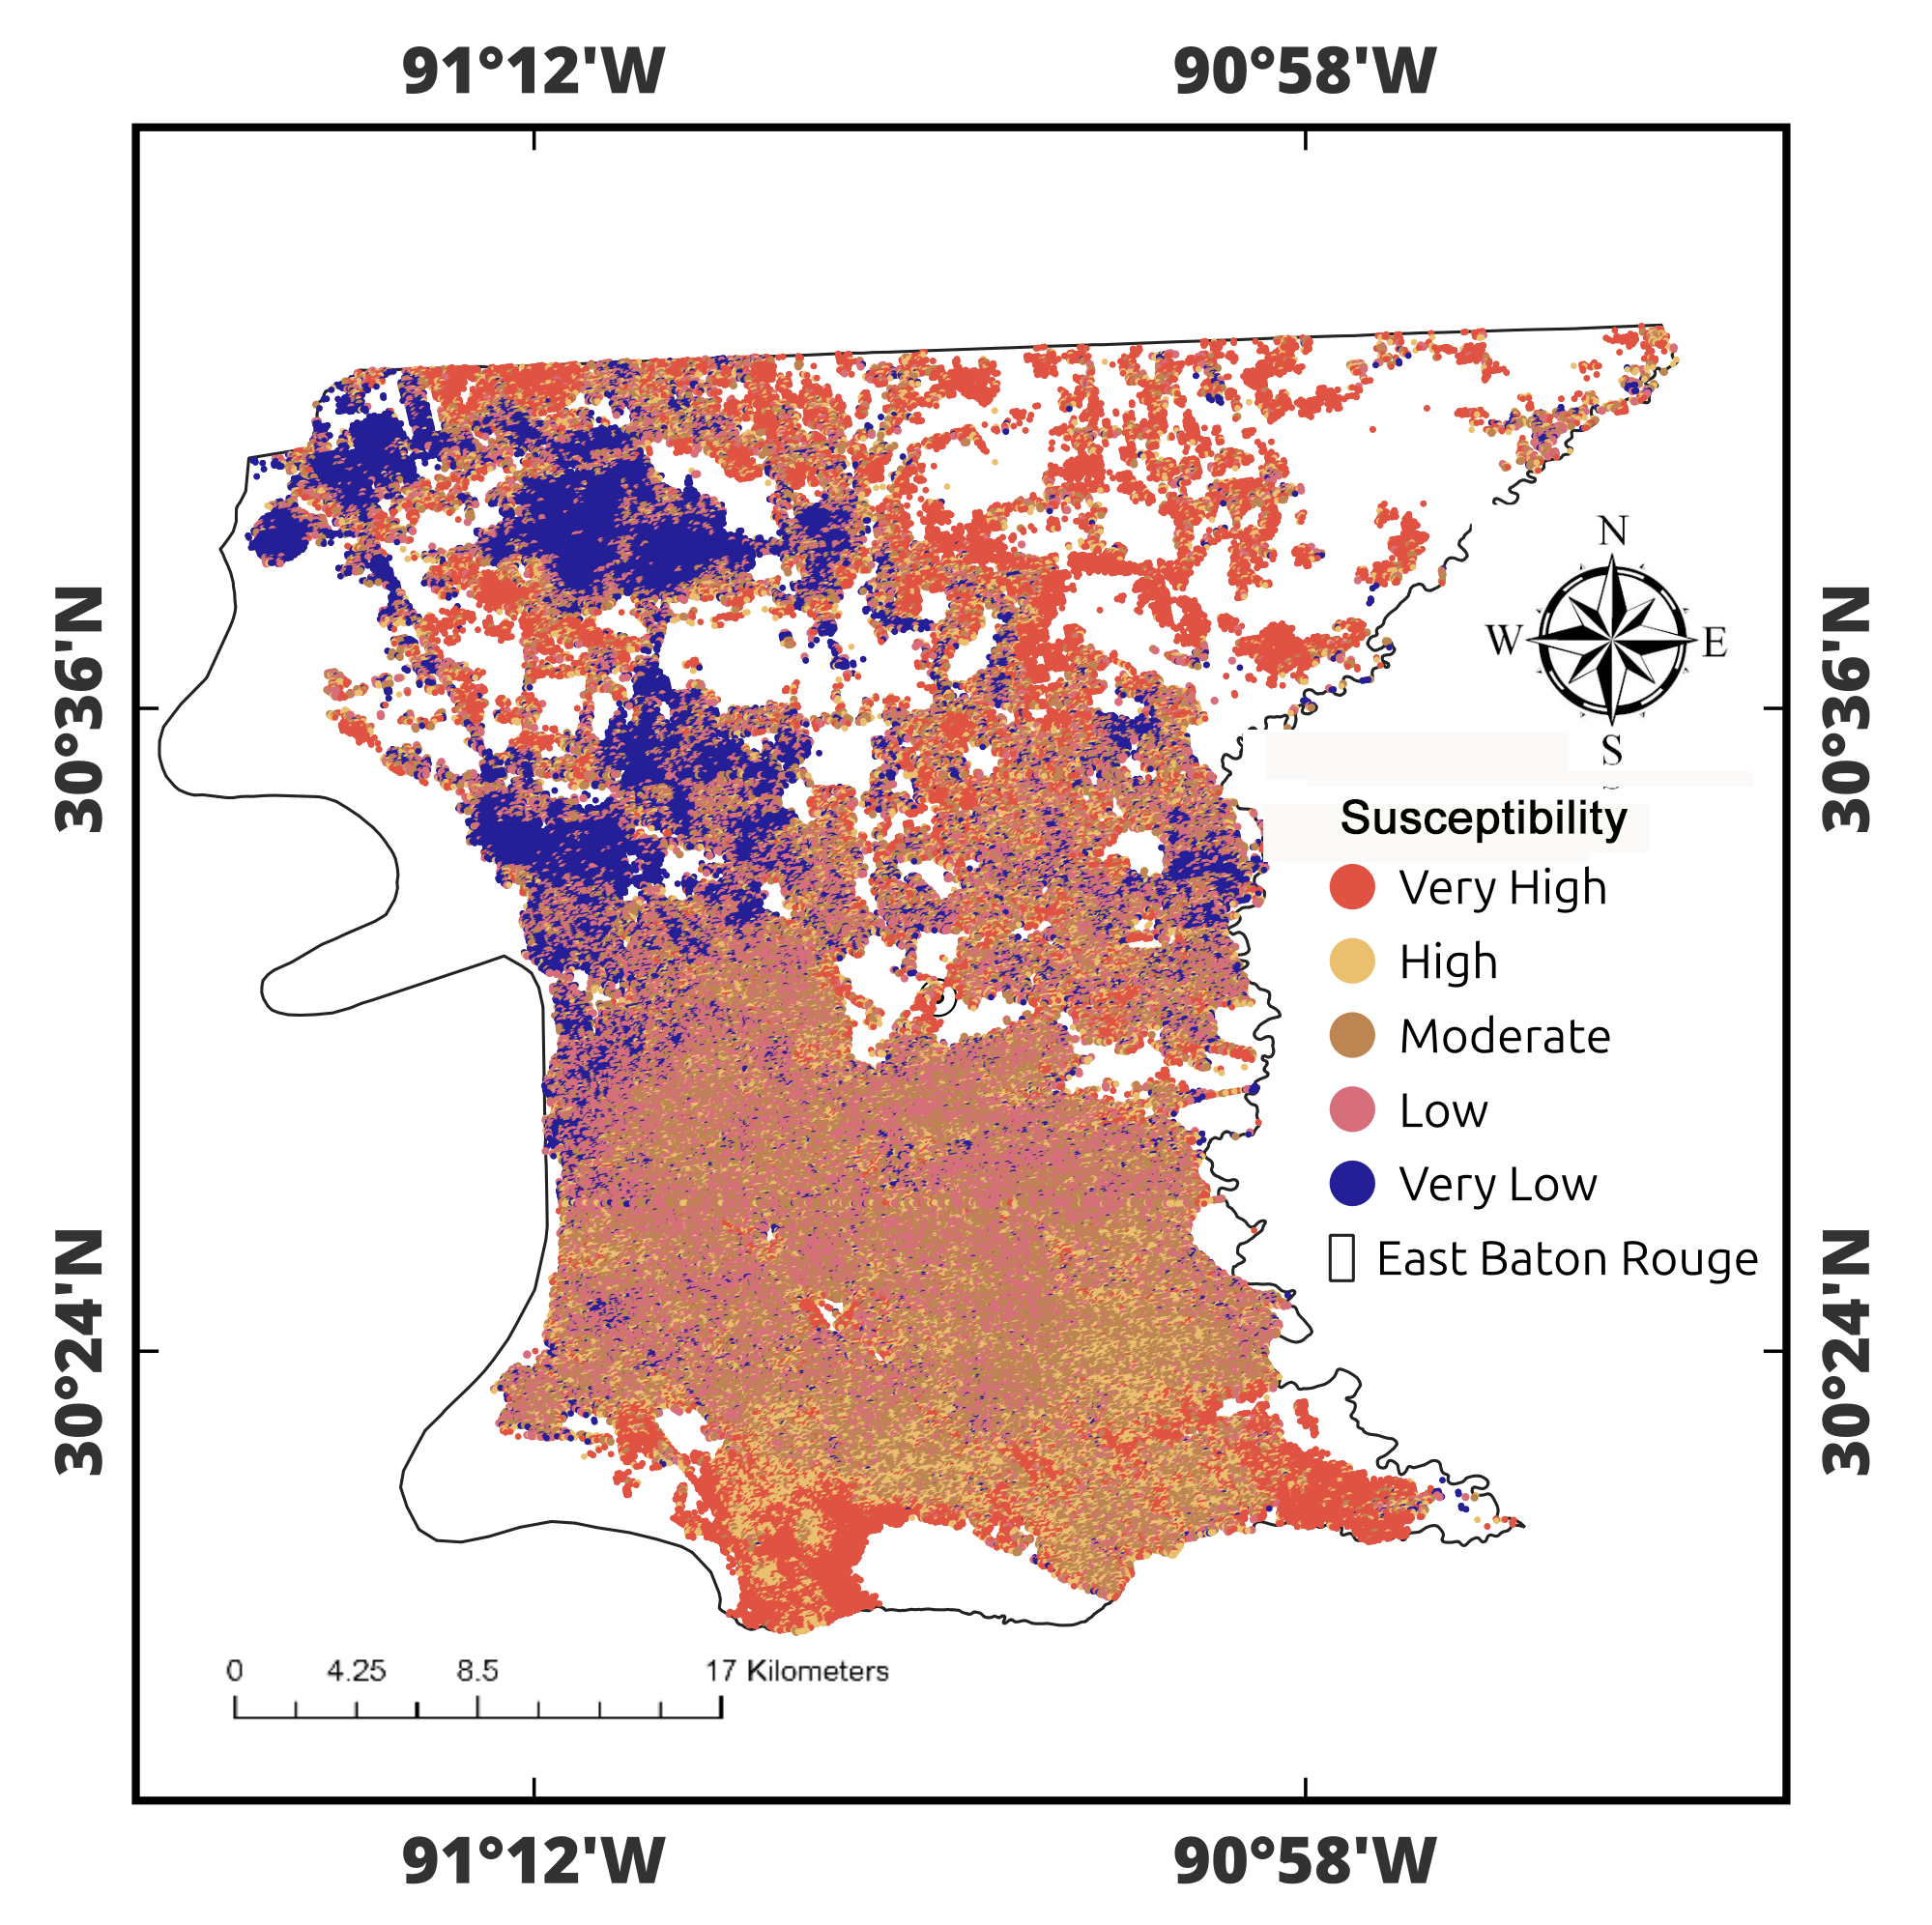
\includegraphics[width=0.48\textwidth]{media/sbas_susc.png} \\
(a) SBAS-InSAR Velocity & (b) SBAS-InSAR Susceptibility
\end{tabular}
\caption{SBAS-InSAR results: (a) Displacement velocity (mm/yr) showing subsidence (red-orange) and uplift (blue); (b) Derived susceptibility classification.}
\label{fig:sbas_results}
\end{figure}

The velocity distribution reveals a clear north-south gradient in deformation patterns. High subsidence rates ($-23.7$ to $-2.1$~mm/yr) concentrate in the southern portions of the parish, while uplift ($3.1$ to $19.2$~mm/yr) dominates the northern forested regions. Moderate deformation zones ($-2.1$ to $3.1$~mm/yr) occupy transitional areas between these extremes. The susceptibility classification correspondingly identifies Very High to High risk zones in the south, transitioning through Moderate risk in central areas to Low and Very Low risk in the north.

\subsection{GNSS Validation}


InSAR displacements were validated against GNSS measurements from three GulfNet CORS stations (Figure~\ref{fig:gnss_validation}). GNSS components were projected into InSAR LOS using:
\begin{equation}
d_{\text{LOS}} = -\sin\theta\cos\alpha \cdot d_E - \sin\theta\sin\alpha \cdot d_N + \cos\theta \cdot d_U
\end{equation}

\begin{figure}[!t]
\centering

\includegraphics[width=0.95\textwidth]{GPS_InSAR_LOS_Validation.png}
\caption{Timeseries Comparison of GPS and InSAR LOS displacement at 1LSU, GVMS, and SJB1 stations. }
\label{fig:gnss_validation}
\end{figure}

\begin{table}[!t]
\centering
\caption{Validation of InSAR-derived velocities against GPS measurements at 1LSU, GVMS, and SJB1 stations}
\label{tab:gnss_validation}
\begin{tabular}{lccc}
\hline
\textbf{Station} & \textbf{GPS-LOS (mm/yr)} & \textbf{InSAR (mm/yr)} & \textbf{RMSE (mm)} \\
\hline
1LSU & $-3.84$ & $-2.21$ & 15.5 \\
GVMS & $-2.59$ & $-6.17$ & 17.5 \\
SJB1 & $-2.29$ & $-3.30$ & 27.1 \\
\hline
\end{tabular}
\end{table}

The time series comparison (Figure~\ref{fig:gnss_validation}) spanning 2017--2025 demonstrates that both GPS and InSAR capture consistent subsidence trends at all three stations. At 1LSU, GPS measured $-3.84$~mm/yr while InSAR recorded $-2.21$~mm/yr (difference of 1.63~mm/yr), yielding a correlation of $r = 0.32$ and RMSE of 15.5~mm. SJB1 showed the closest velocity agreement, with GPS at $-2.29$~mm/yr versus InSAR at $-3.30$~mm/yr (difference of 1.01~mm/yr), though with lower temporal correlation ($r = 0.33$, RMSE = 27.1~mm). GVMS exhibited the strongest temporal correlation ($r = 0.65$, RMSE = 17.5~mm), indicating good pattern agreement despite the largest velocity difference (GPS: $-2.59$~mm/yr, InSAR: $-6.17$~mm/yr, difference of 3.58~mm/yr).

Both techniques reveal consistent linear subsidence trends throughout the 8-year monitoring period, with seasonal variability evident in GPS data. The moderate correlations are attributed to spatial separation between stations and InSAR pixels, differences in 3D versus line-of-sight measurement sensitivity, and tropospheric artifacts \citep{Crosetto2016}. Despite velocity differences, both GPS and InSAR confirm subsidence at all stations, validating SBAS-InSAR reliability for regional monitoring.


\section{Spatial Susceptibility Mapping}

Both Extra Trees (ET) and Random Forest (RF) regressors were trained on the augmented dataset comprising 393,412 samples derived from SBAS-InSAR velocities and 15 environmental conditioning factors. Model development employed 5-fold cross-validation with hyperparameter optimization. Table~\ref{tab:model_performance} summarizes performance metrics on the held-out test set.

ET achieved superior performance across all metrics, with test $R^2 = 0.9236$ compared to RF ($R^2 = 0.8825$). This difference ($\Delta R^2 = 0.041$) is statistically significant ($p < 0.001$), confirming that ET provides better generalization for subsidence prediction in EBRP. The improved performance is attributable to ET's random threshold splitting mechanism, which introduces additional randomization at node splits, reducing overfitting and enhancing robustness to multicollinear predictors \citep{Geurts2006}. Similar findings have been reported in other geohazard susceptibility studies where ET outperformed conventional RF \citep{Gharechaee2023}.

\begin{table}[!t]
\centering
\caption{Extra Trees (ET) and Random Forest (RF) model performance comparison}
\label{tab:model_performance}
\begin{tabular}{lccc}
\hline
\textbf{Model} & \textbf{$R^2$} & \textbf{RMSE (mm/yr)} & \textbf{MAE (mm/yr)} \\
\hline
Extra Trees    & 0.9236 & 1.10 & 0.72 \\
Random Forest  & 0.8825 & 1.37 & 1.03 \\
\hline
\end{tabular}
\end{table}

The optimized models were applied to generate spatially continuous maps. The Extra Trees velocity map (Figure~\ref{fig:et_results}a) shows predicted velocities ranging from $-23.3$ to $+19.2$~mm/yr, closely matching the SBAS-InSAR observed range ($-23.7$ to $+19.2$~mm/yr). This strong agreement demonstrates that the selected environmental conditioning factors effectively capture the physical drivers of subsidence in EBRP. High subsidence ($-23.3$ to $-2$~mm/yr) concentrates in the southern parish, moderate zones ($-2$ to $1.4$~mm/yr) occupy transitional areas, and uplift ($3$ to $19.2$~mm/yr) dominates the northern forested regions.

\begin{figure}[!t]
\centering
\begin{tabular}{cc}
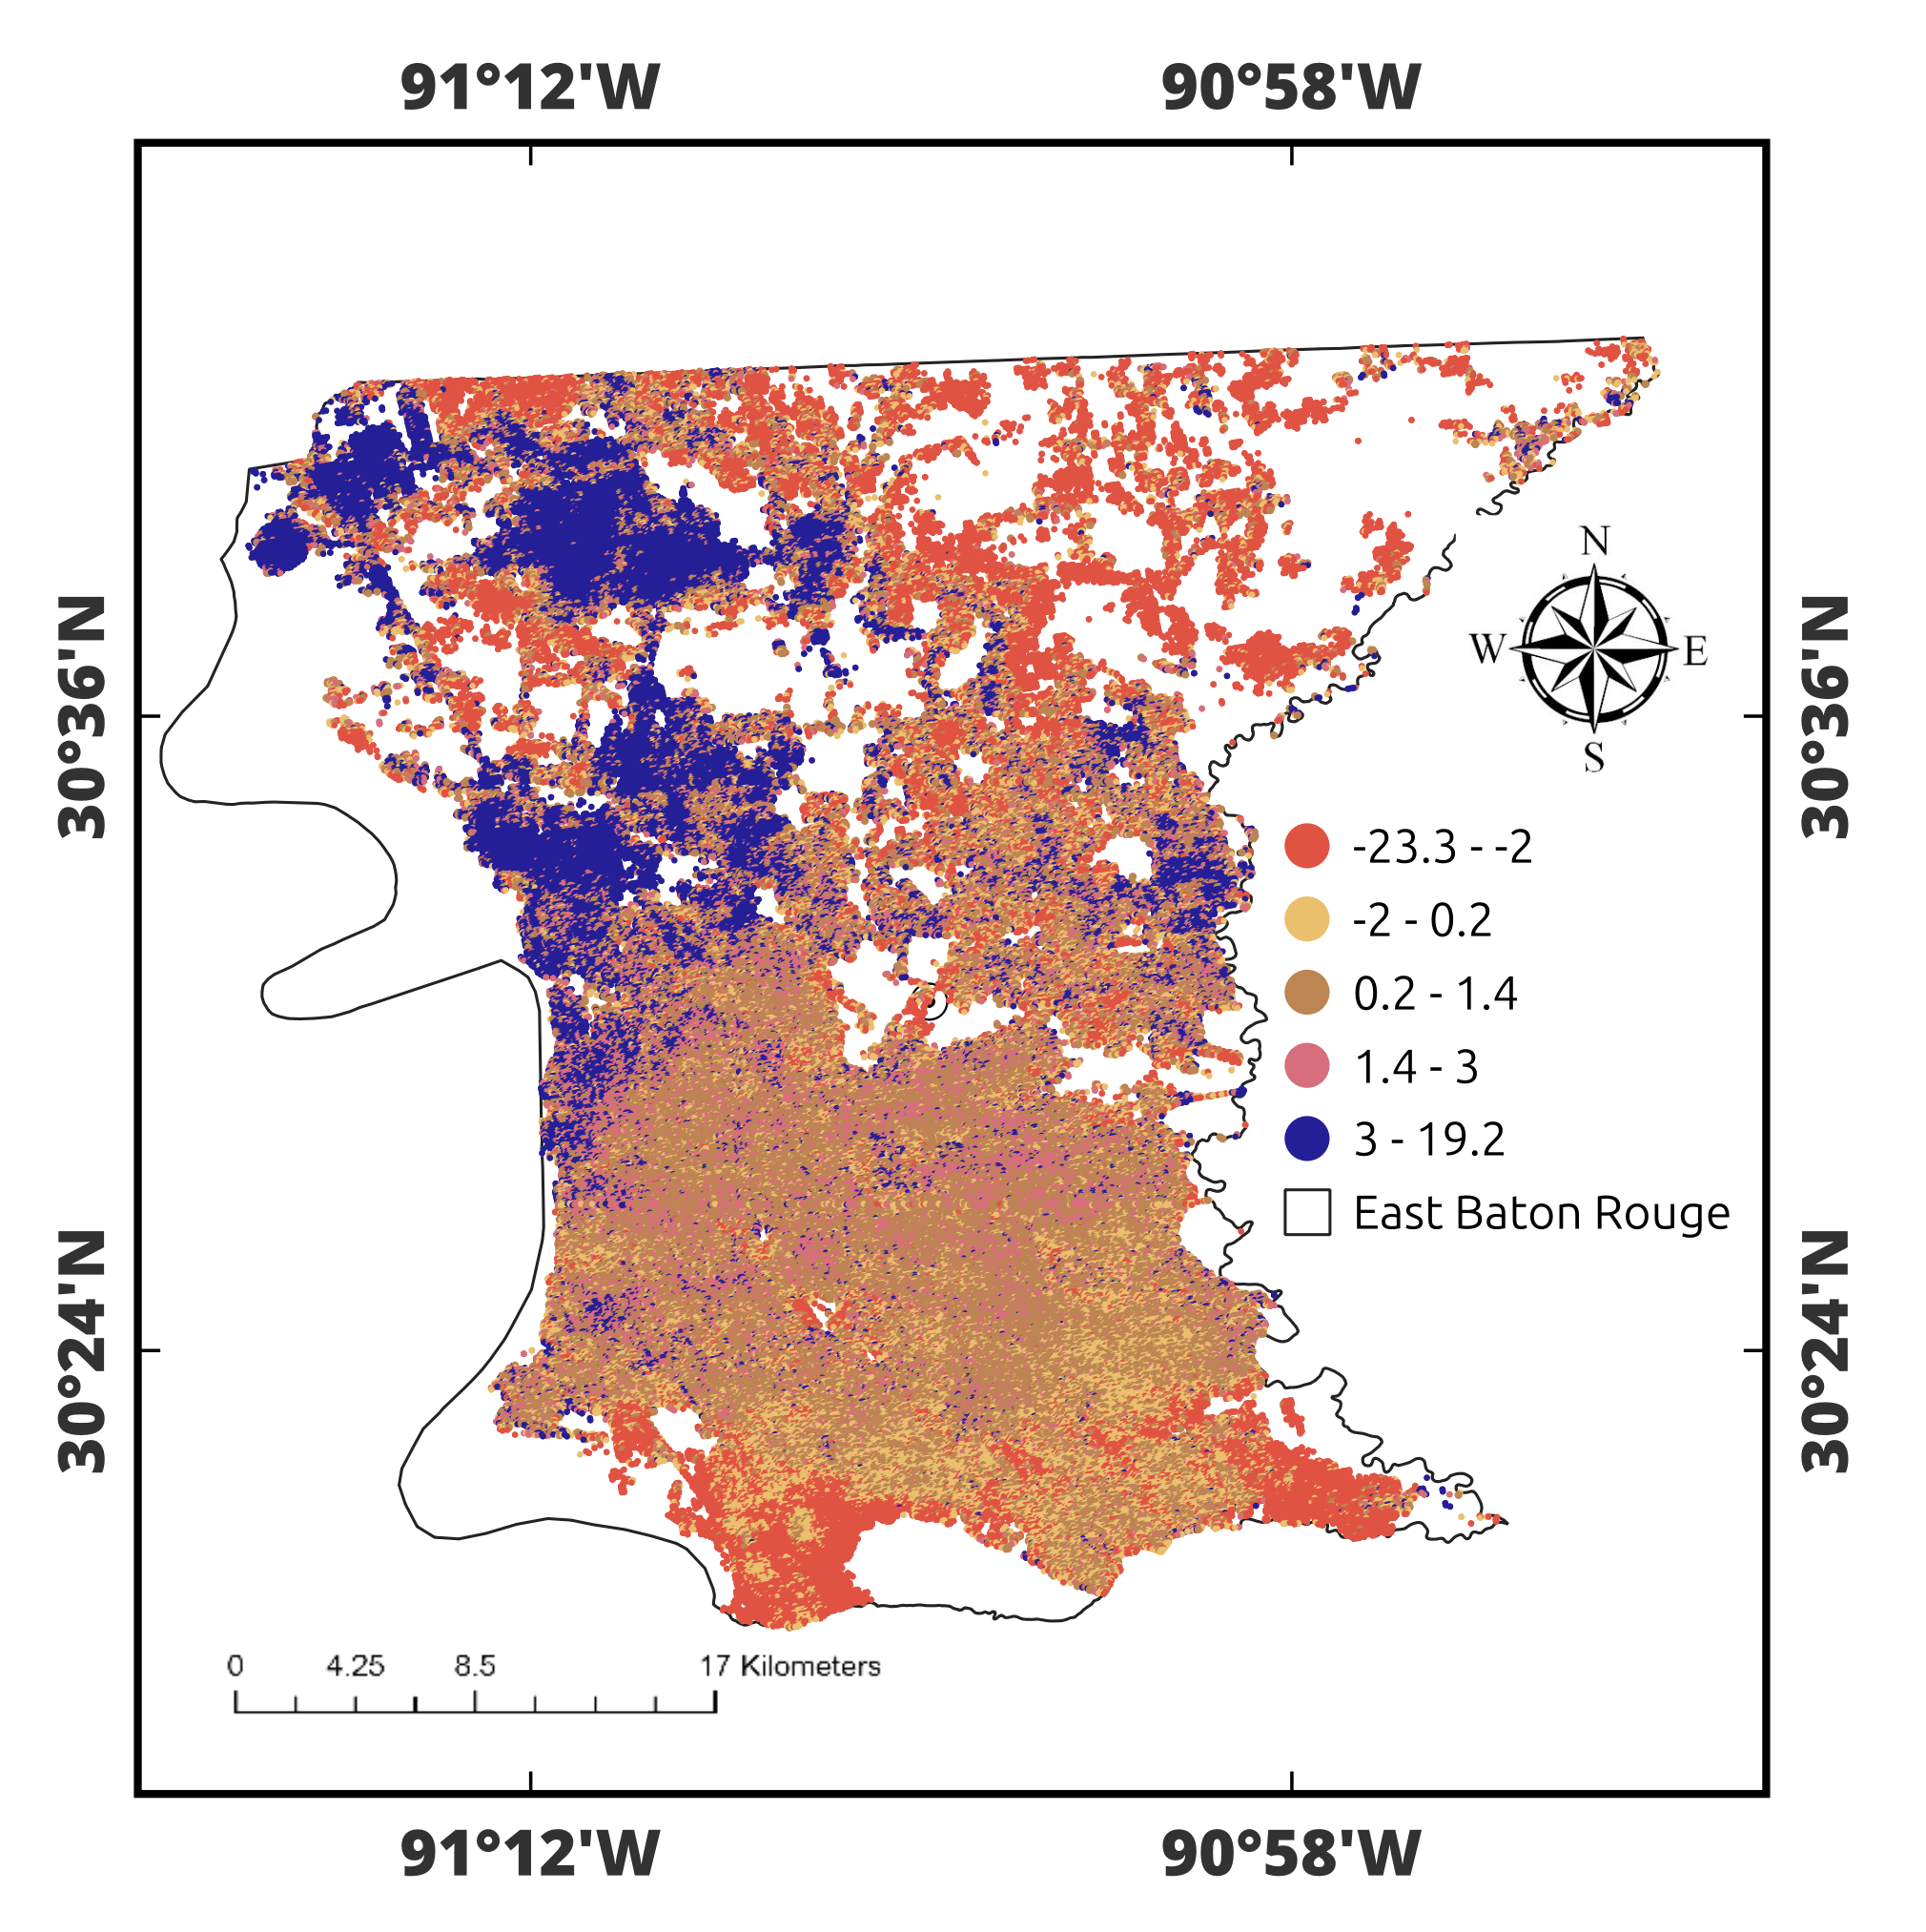
\includegraphics[width=0.48\textwidth]{media/et_vel.png} &
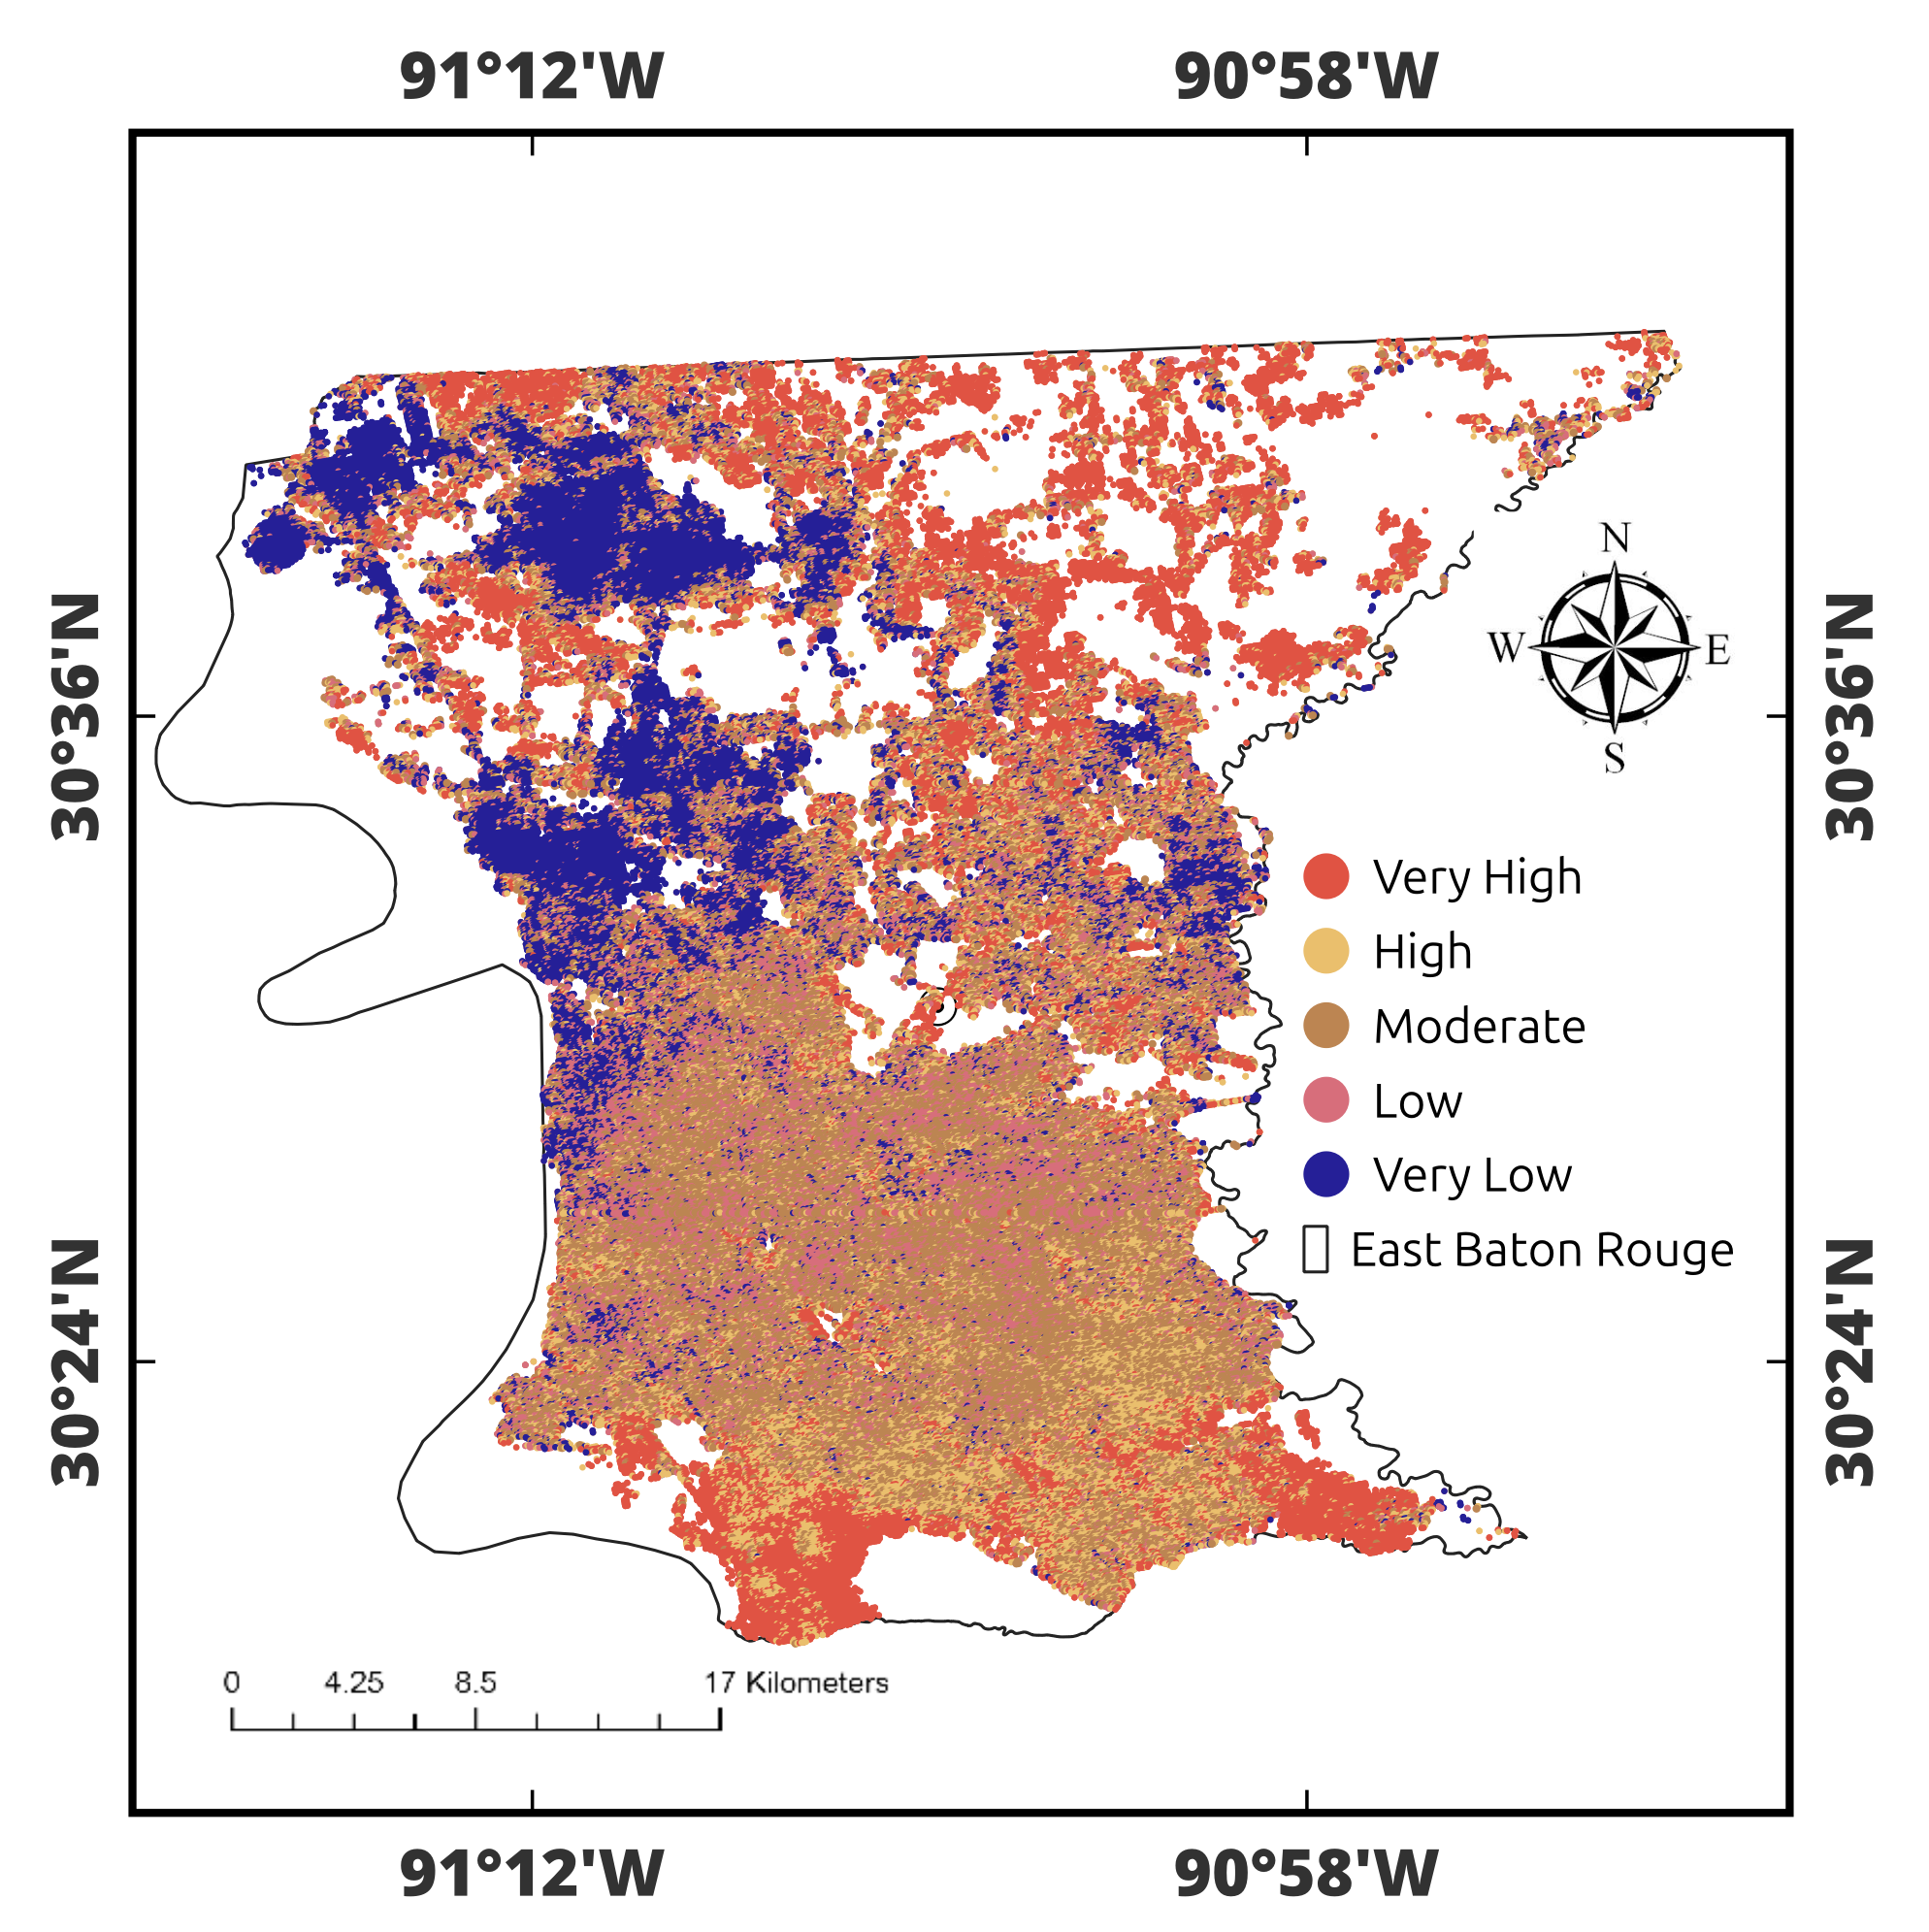
\includegraphics[width=0.48\textwidth]{media/et_susc.png} \\
(a) Extra Trees Predicted Velocity & (b) Extra Trees Susceptibility
\end{tabular}
\caption{Extra Trees model results: (a) Predicted velocity (mm/yr); (b) Susceptibility classification. High-risk zones concentrate along the southern urban corridor and fault-proximal areas.}
\label{fig:et_results}
\end{figure}

\begin{figure}[!t]
\centering
\begin{tabular}{cc}
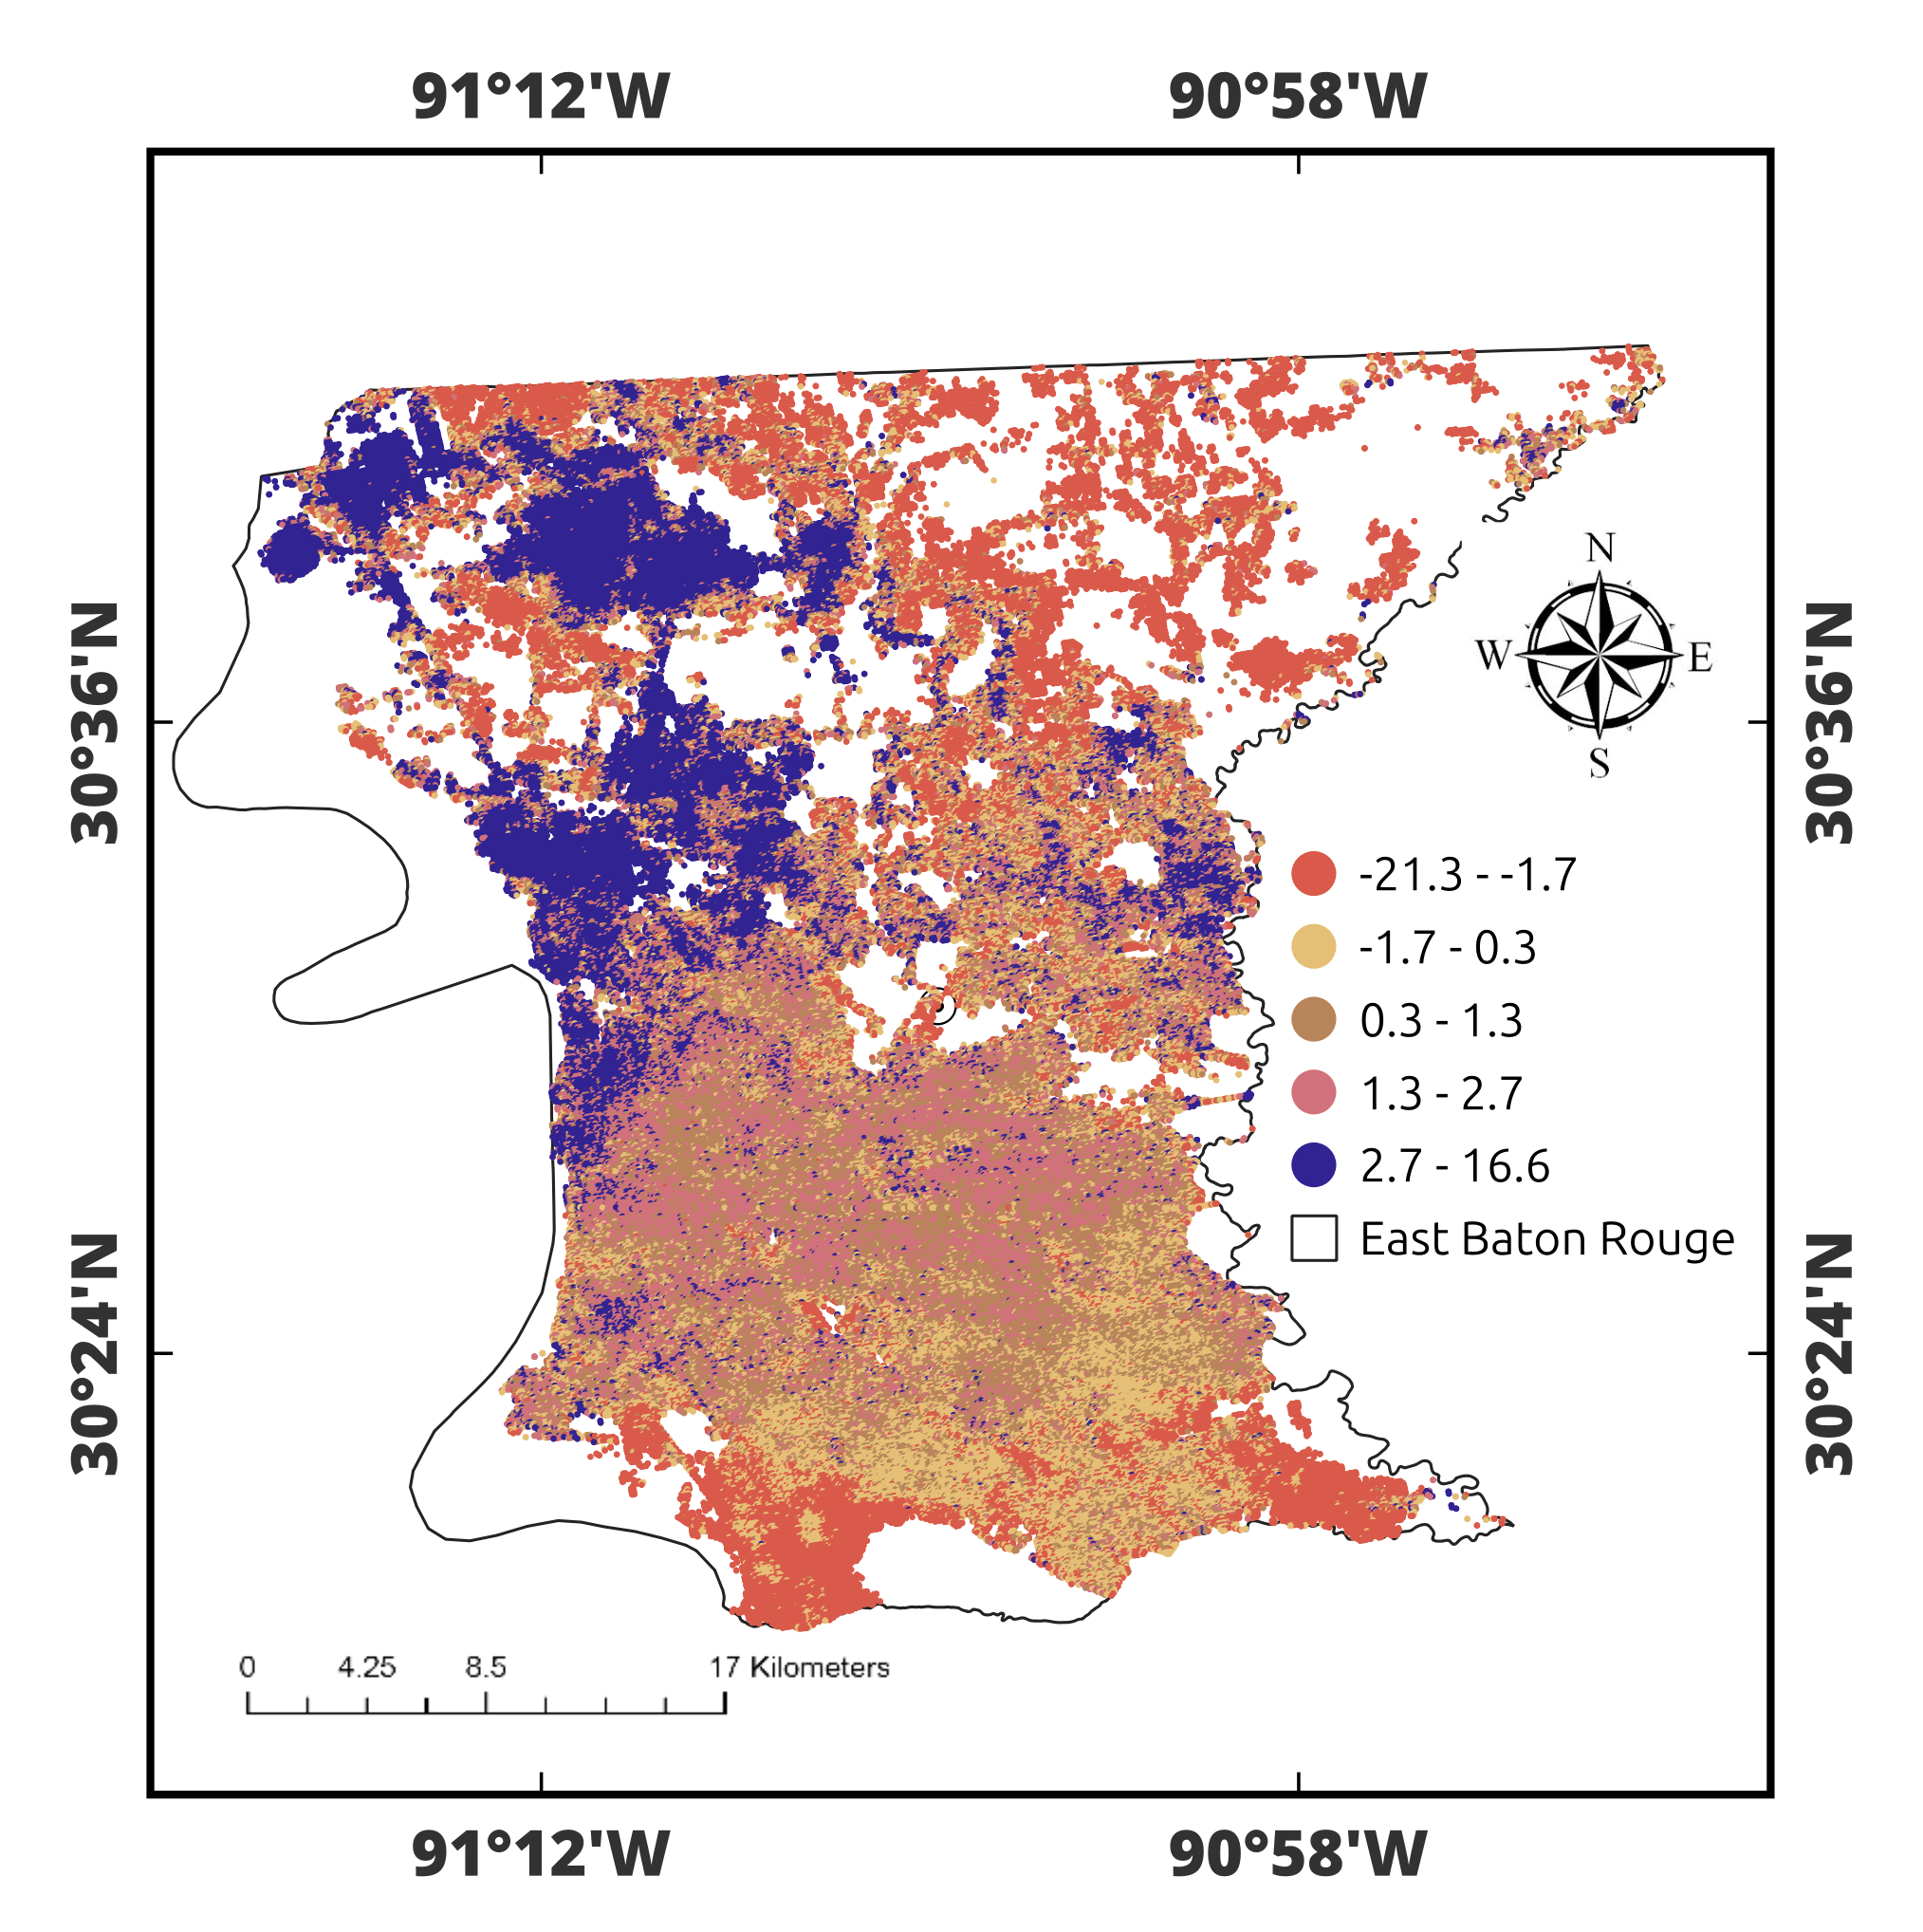
\includegraphics[width=0.48\textwidth]{media/rf_vel.png} &
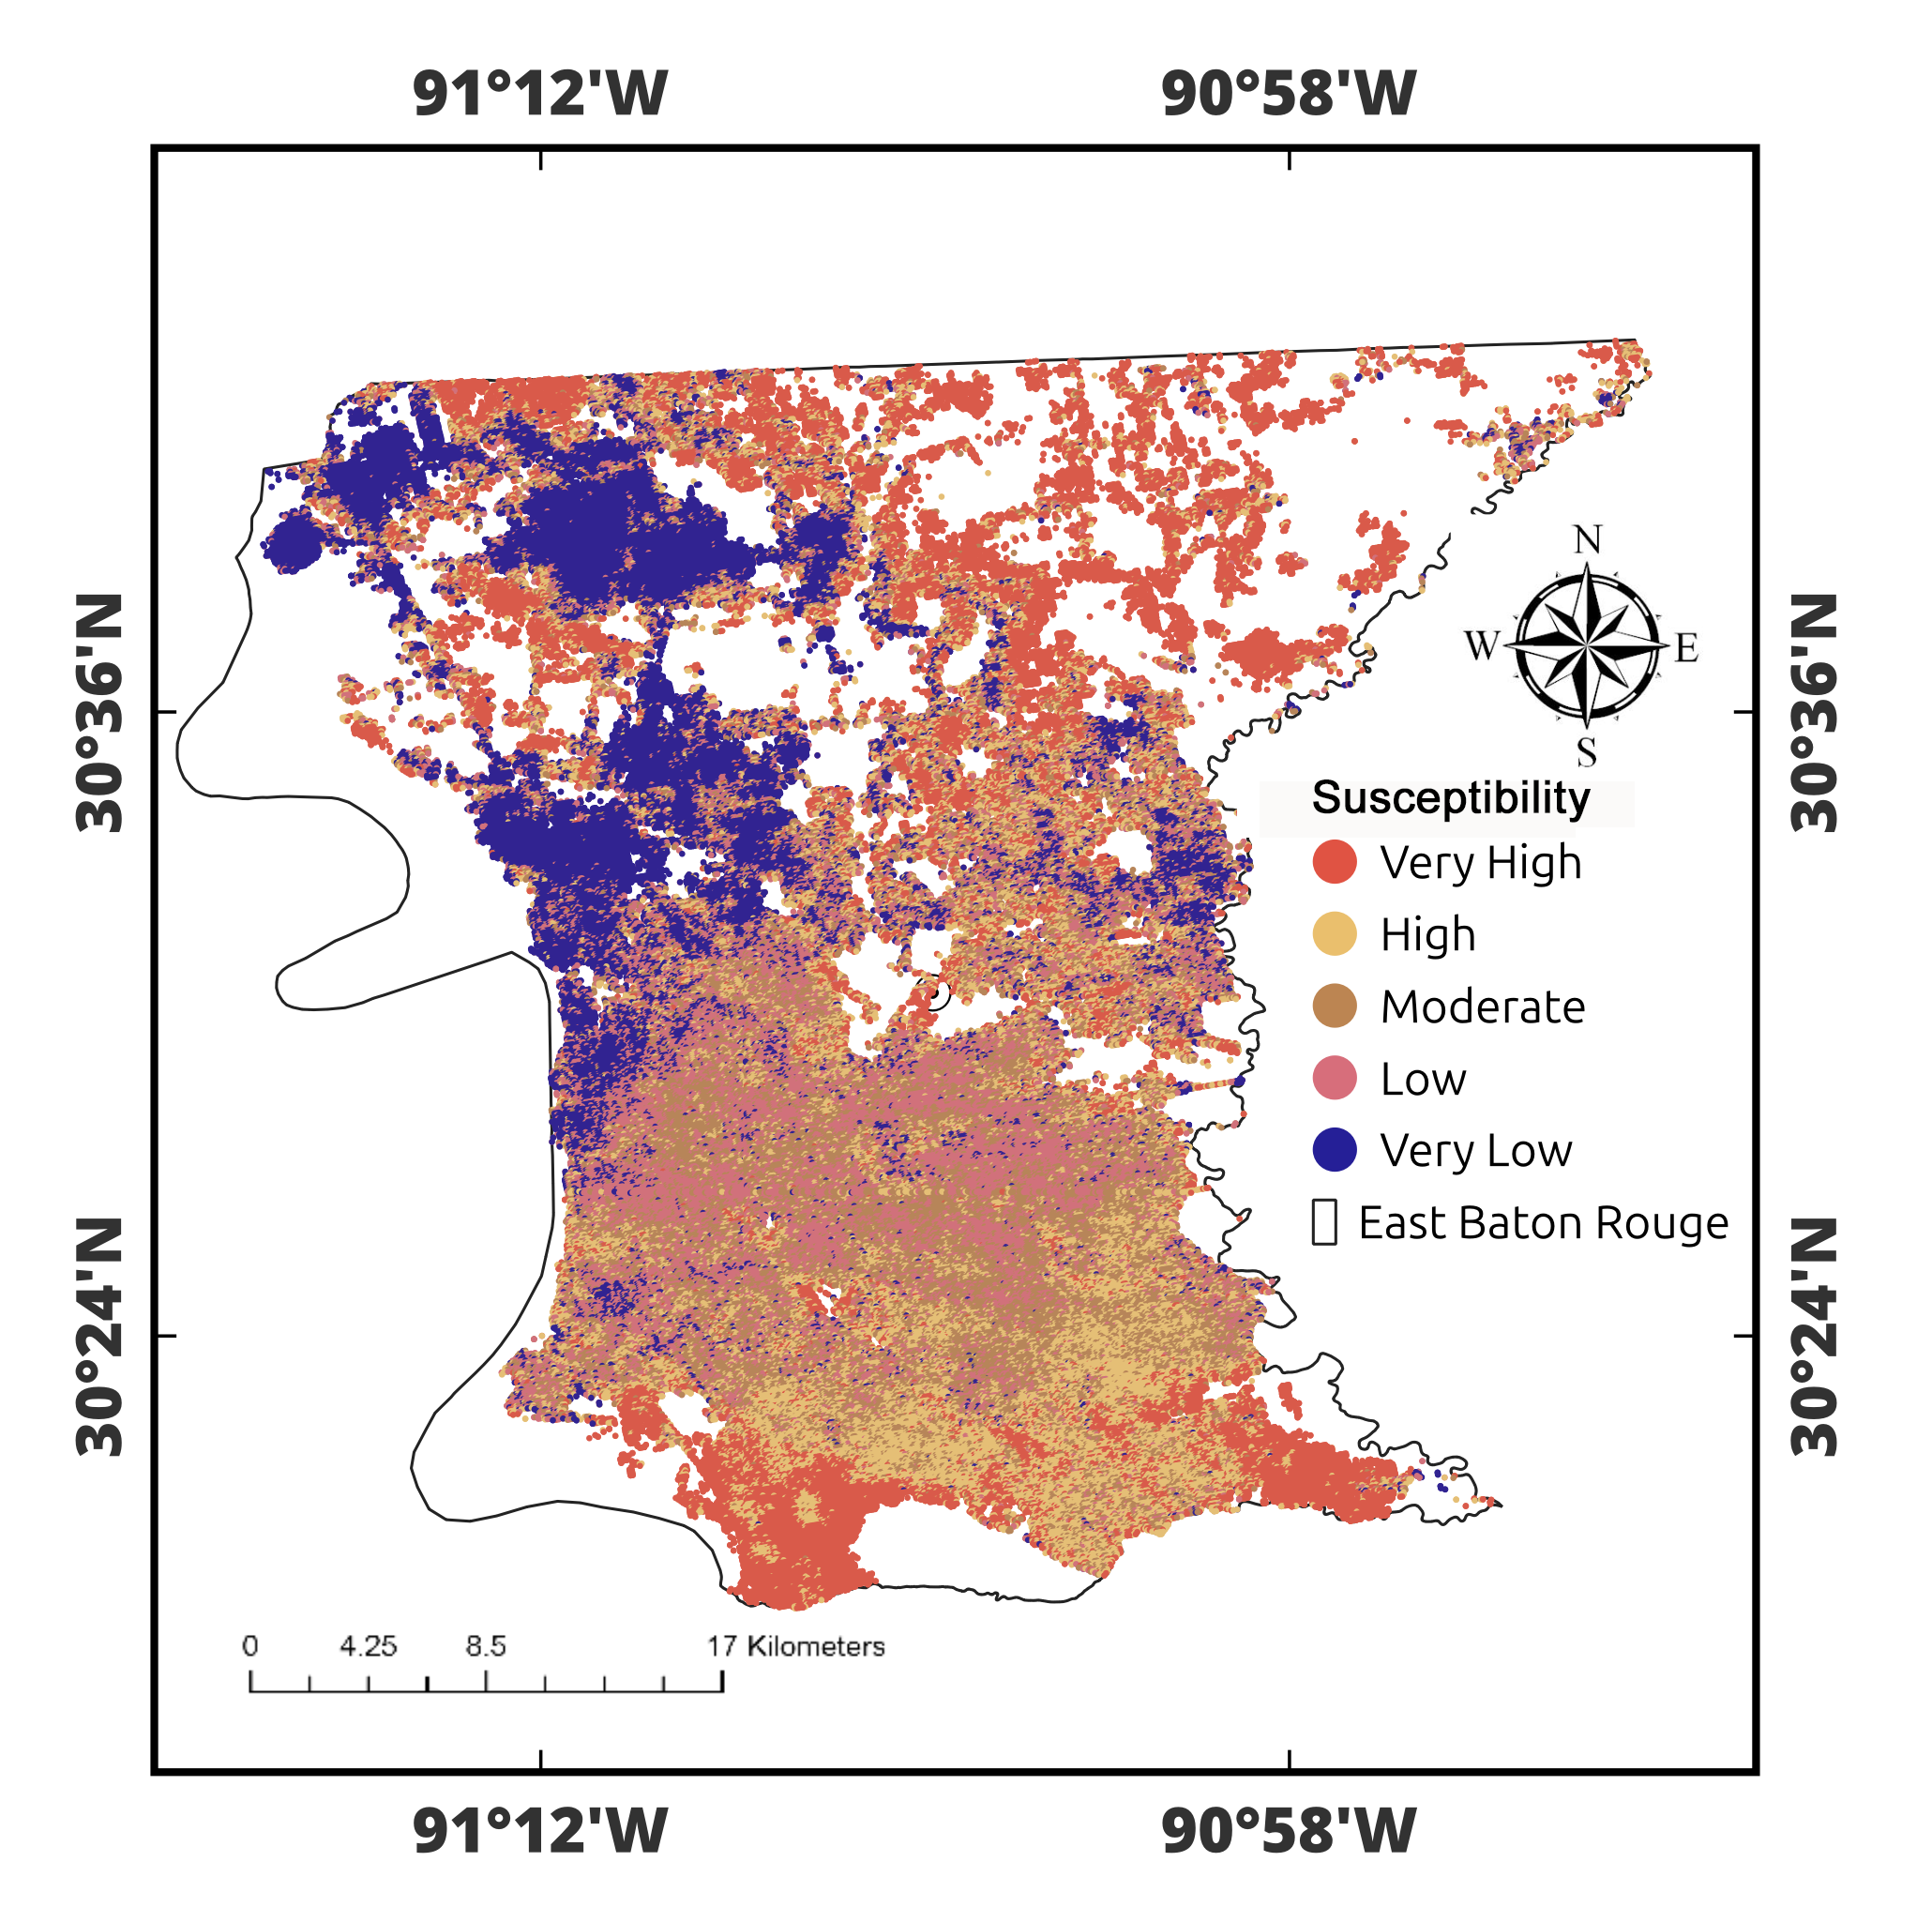
\includegraphics[width=0.48\textwidth]{media/rf_susc.png} \\
(a) Random Forest Predicted Velocity & (b) Random Forest Susceptibility
\end{tabular}
\caption{Random Forest model results: (a) Predicted velocity (mm/yr); (b) Susceptibility classification. Spatial patterns are similar to ET but with less pronounced gradients.}
\label{fig:rf_results}
\end{figure}

The Random Forest velocity map (Figure~\ref{fig:rf_results}a) shows predicted velocities ranging from $-21.3$ to $+16.6$~mm/yr, with high subsidence ($-21.3$ to $-1.7$~mm/yr) in the southern parish, moderate zones ($-1.7$ to $1.3$~mm/yr) in transitional areas, and uplift ($2.7$ to $16.6$~mm/yr) in the northern regions. The corresponding susceptibility classification (Figure~\ref{fig:rf_results}b) identifies the same five risk levels as ET. Both models exhibit consistent spatial patterns, with the southern urban corridor and fault-proximal areas classified as Very High to High risk, while northern forested areas show Low to Very Low susceptibility.

In summary, SBAS-InSAR observed velocities from $-23.7$ to $+19.2$~mm/yr, while ET predicted $-23.3$ to $+19.2$~mm/yr ($R^2 = 0.9236$) and RF predicted $-21.3$ to $+16.6$~mm/yr ($R^2 = 0.8825$). All three approaches consistently identify subsidence concentrated in the southern urban corridor and fault-proximal areas, with uplift dominating the northern forested regions. The close agreement between observed SBAS-InSAR patterns and ML predictions confirms that the environmental conditioning factors effectively explain subsidence variability in EBRP.


\section{Feature Importance Analysis}

Understanding the relative contribution of conditioning factors to subsidence susceptibility is essential for developing targeted mitigation strategies. Three complementary explainability techniques MDI, SHAP, and LIME were applied to quantify feature importance and reveal the physical mechanisms driving subsidence in EBRP.

MDI-based feature importance rankings (Figure~\ref{fig:mdi_importance}) reveal model-specific predictor hierarchies. For Extra Trees (Figure~\ref{fig:mdi_importance}a), the top predictors are LULC, DTF, DTRd, DTRDEM, DTR, and DEM. For Random Forest (Figure~\ref{fig:mdi_importance}b), the ranking differs: DTFDEM, DEM, LULC, DTRd, DTRDEM, and DTF. Despite ranking differences, both models consistently identify LULC, fault proximity (DTF), elevation (DEM), and interaction terms (DTRDEM, DTFDEM) as dominant controls, confirming that subsidence is driven by coupled anthropogenic and geological factors.

\begin{figure}[!t]
\centering
\begin{tabular}{cc}
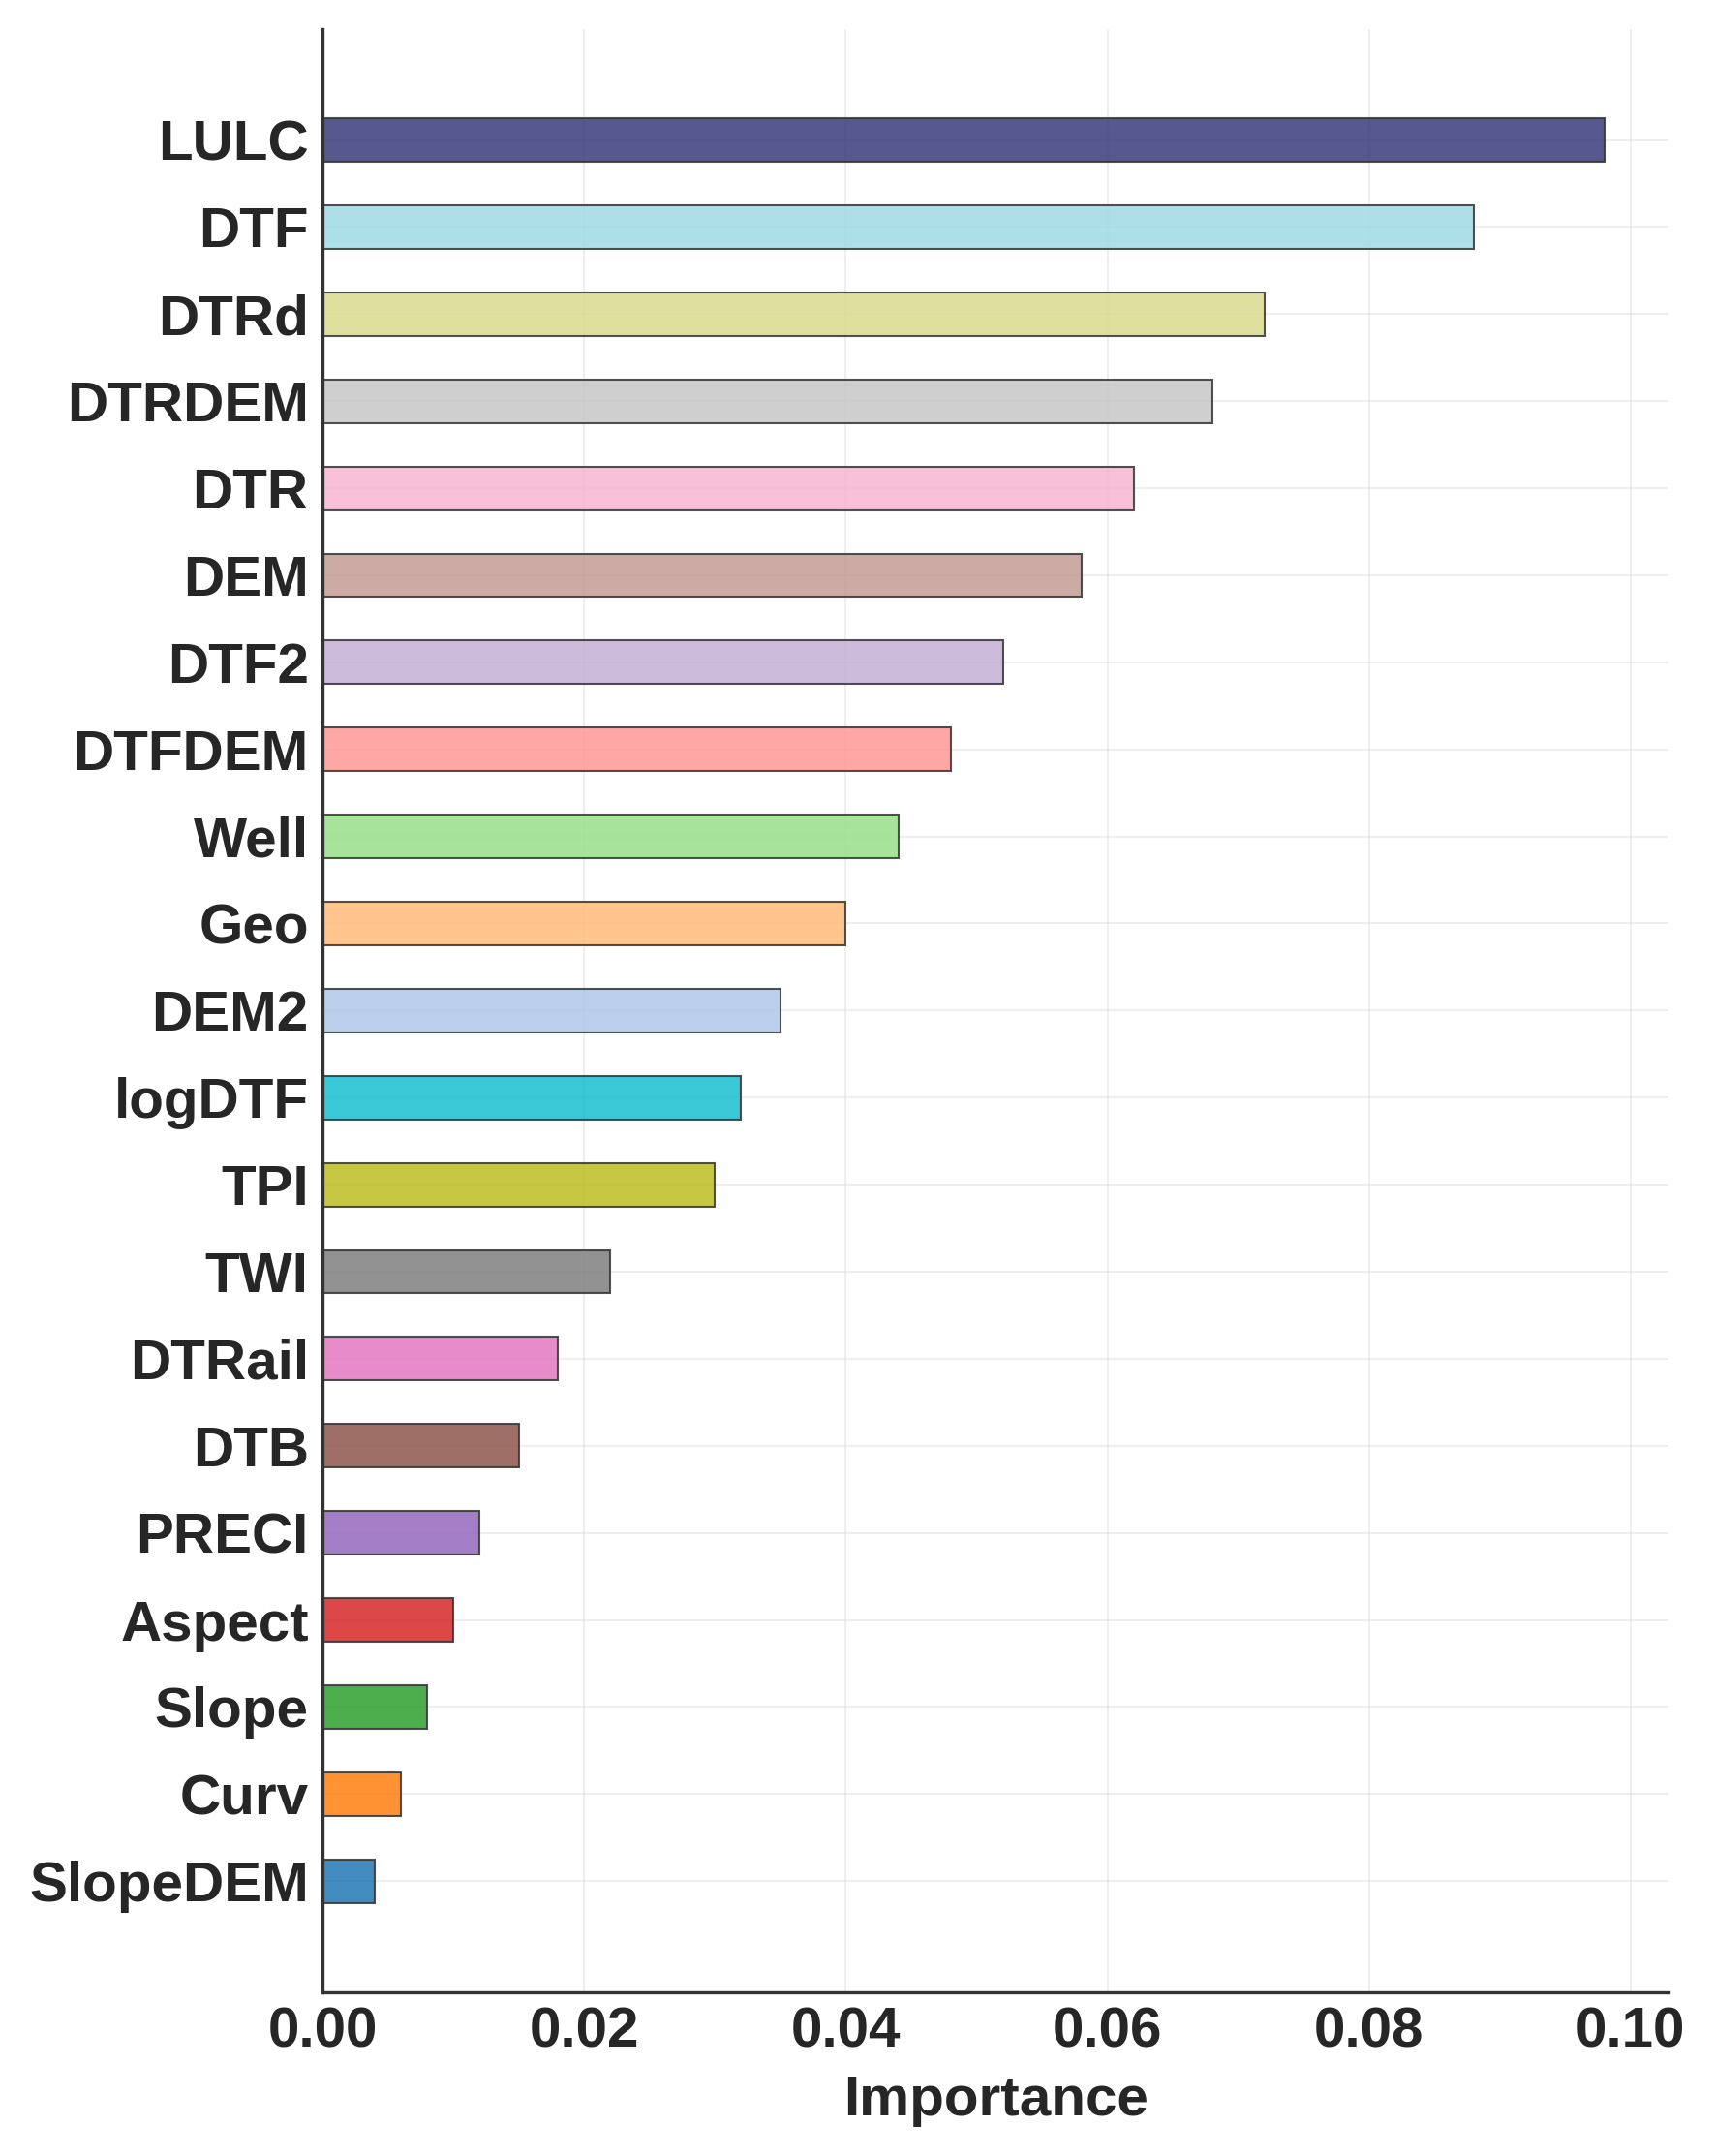
\includegraphics[width=0.48\textwidth]{media/mdi_imp_et_slim.png} &
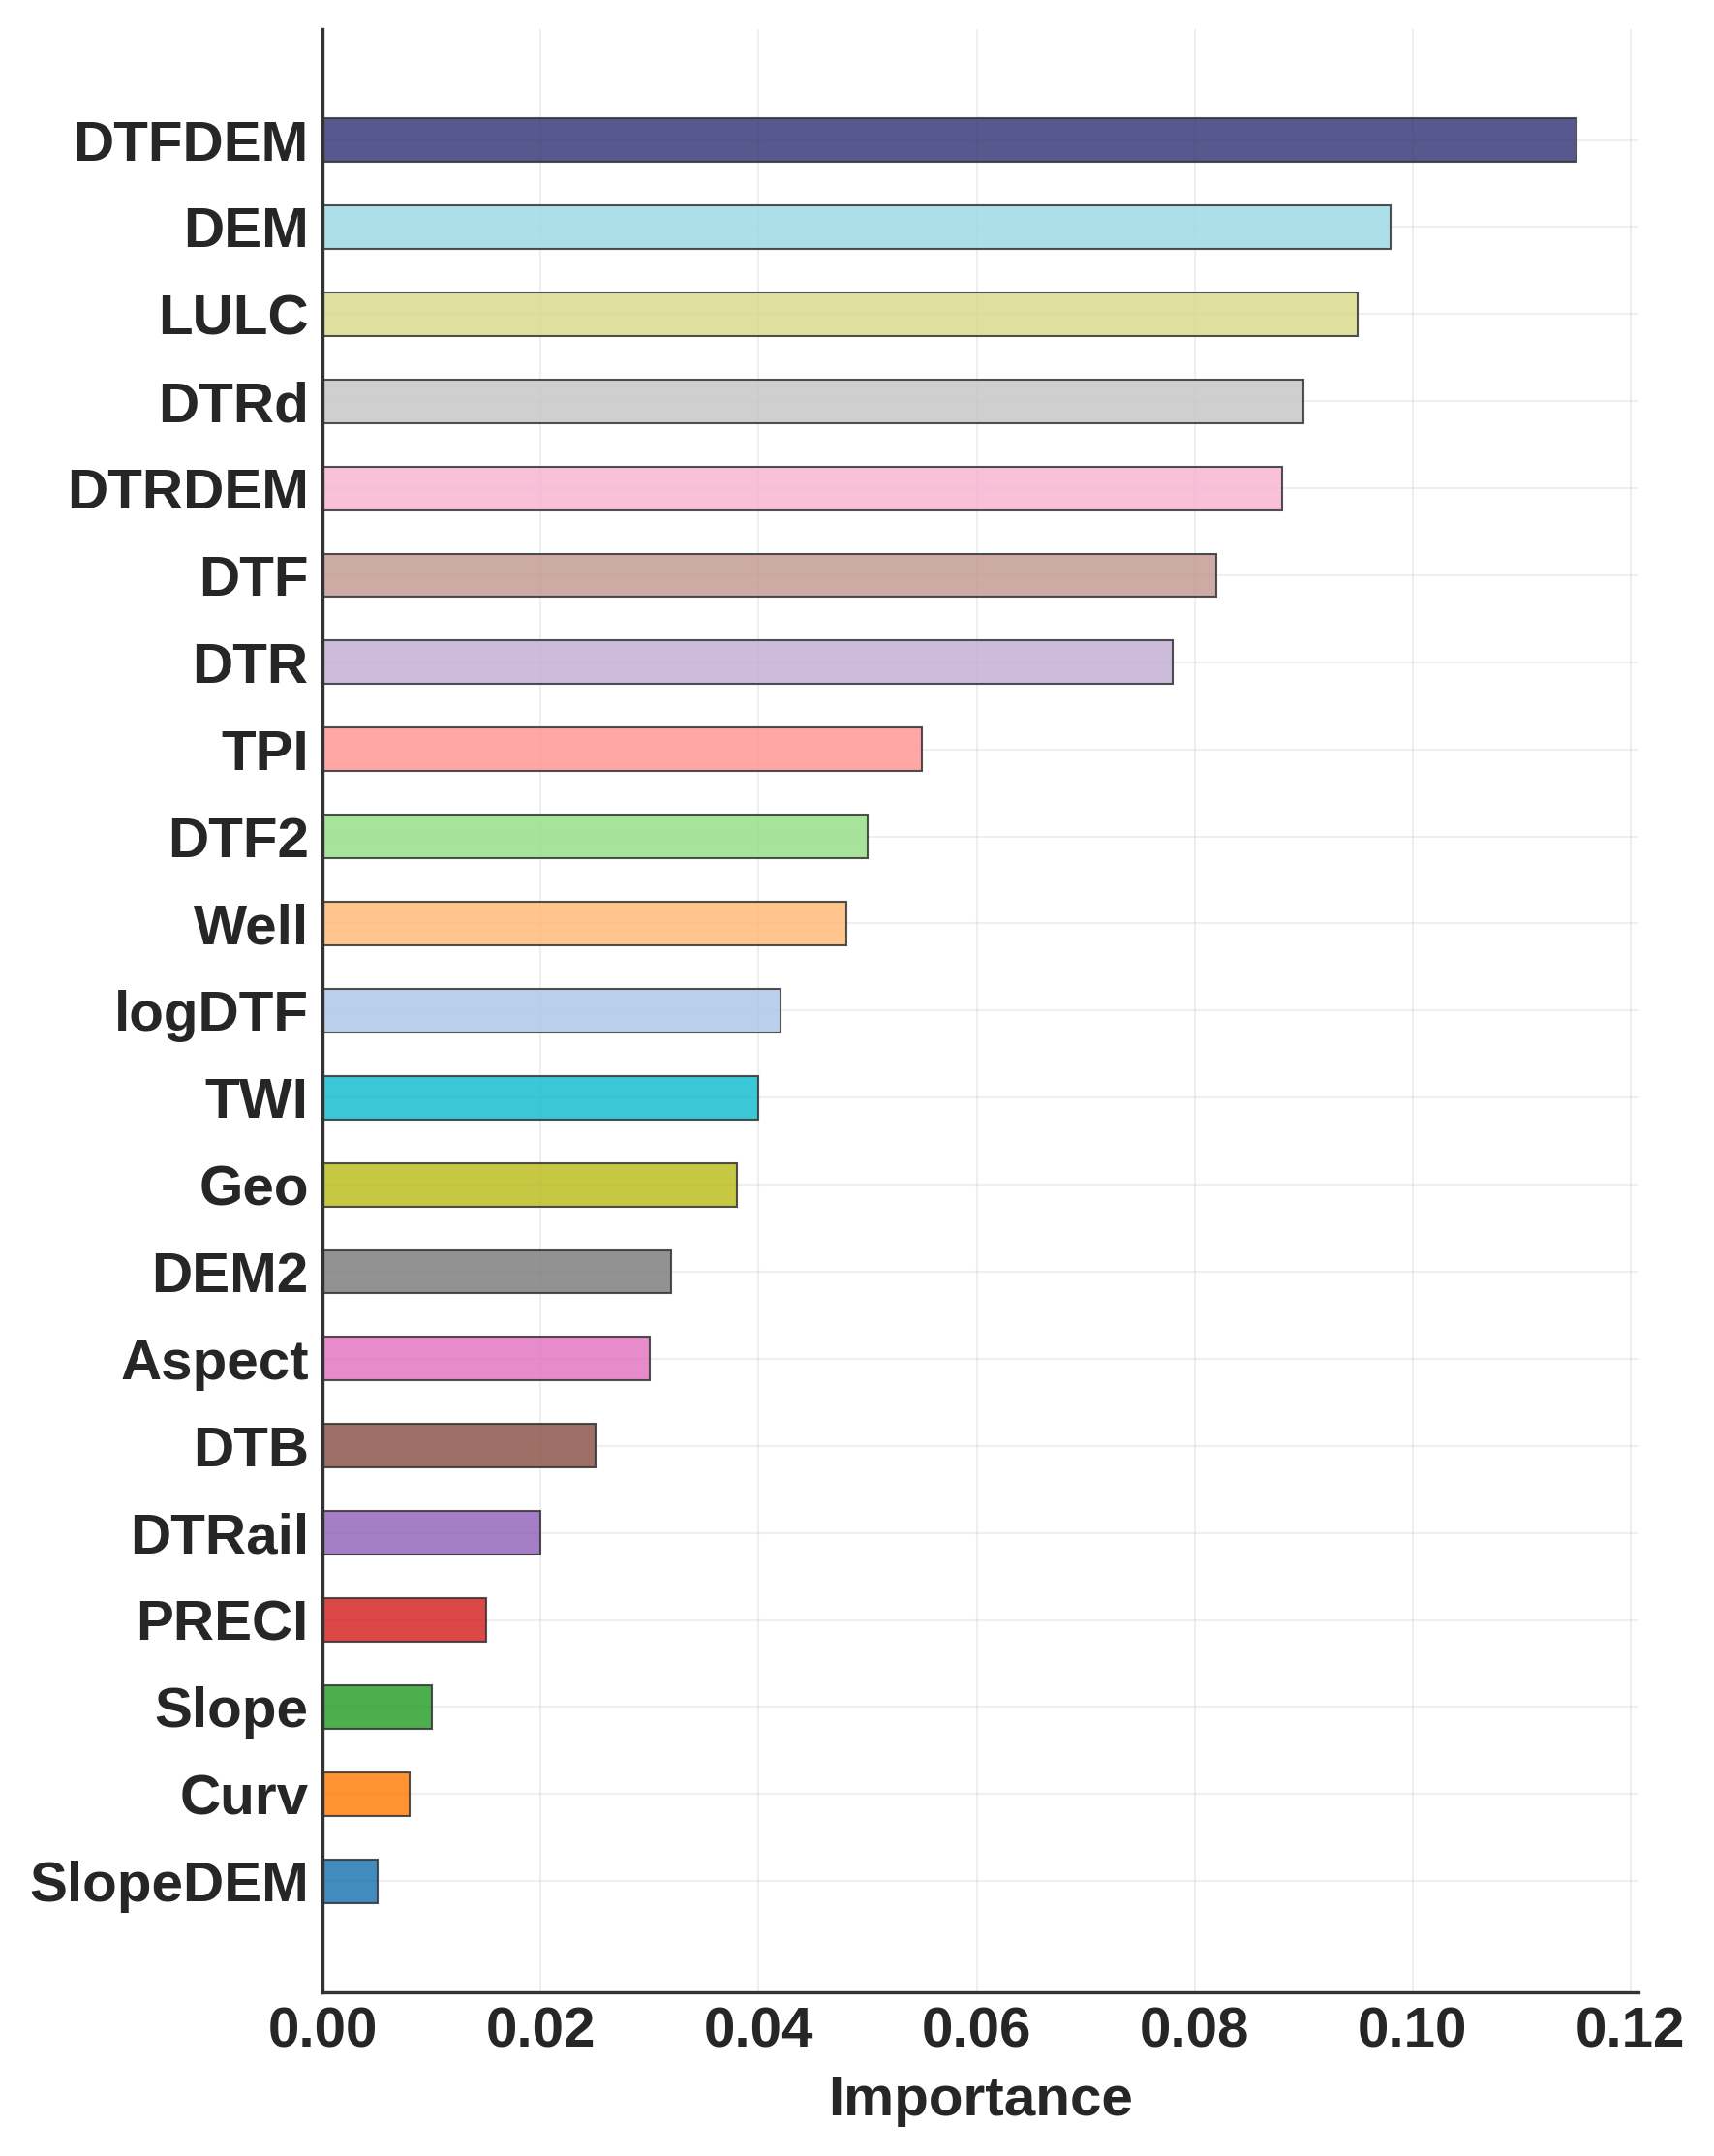
\includegraphics[width=0.48\textwidth]{media/mdi_imp_rf_slim.png} \\
(a) MDI (Extra Trees) & (b) MDI (Random Forest)
\end{tabular}
\caption{MDI-based feature importance: (a) Extra Trees; (b) Random Forest. Both models consistently identify LULC, fault proximity, and topographic-hydrological interactions as dominant controls.}
\label{fig:mdi_importance}
\end{figure}

SHAP analysis (Figures~\ref{fig:shap_summary} and \ref{fig:shap_bar}) provides deeper insight into directional effects and nonlinear relationships. LULC exhibits the highest mean absolute SHAP value, with urban and agricultural classes showing positive contributions (increased subsidence) and forested areas showing negative contributions (reduced subsidence). This pattern confirms that urbanization enhances susceptibility through reduced infiltration, concentrated loading, and localized groundwater demand.

Distance to faults (DTF) shows that closer proximity to fault systems generates positive SHAP values contributing to increased subsidence, while greater distances yield near-zero contributions. This indicates fault-related influences on subsidence are spatially concentrated near fault traces.

The DTRDEM interaction reveals that low-elevation areas near rivers exhibit positive SHAP contributions, indicating that elevation modulates hydrological influences on subsidence. Well influence consistently produces positive SHAP values, confirming groundwater extraction as a key anthropogenic driver.

\begin{figure}[!t]
\centering
\begin{tabular}{cc}
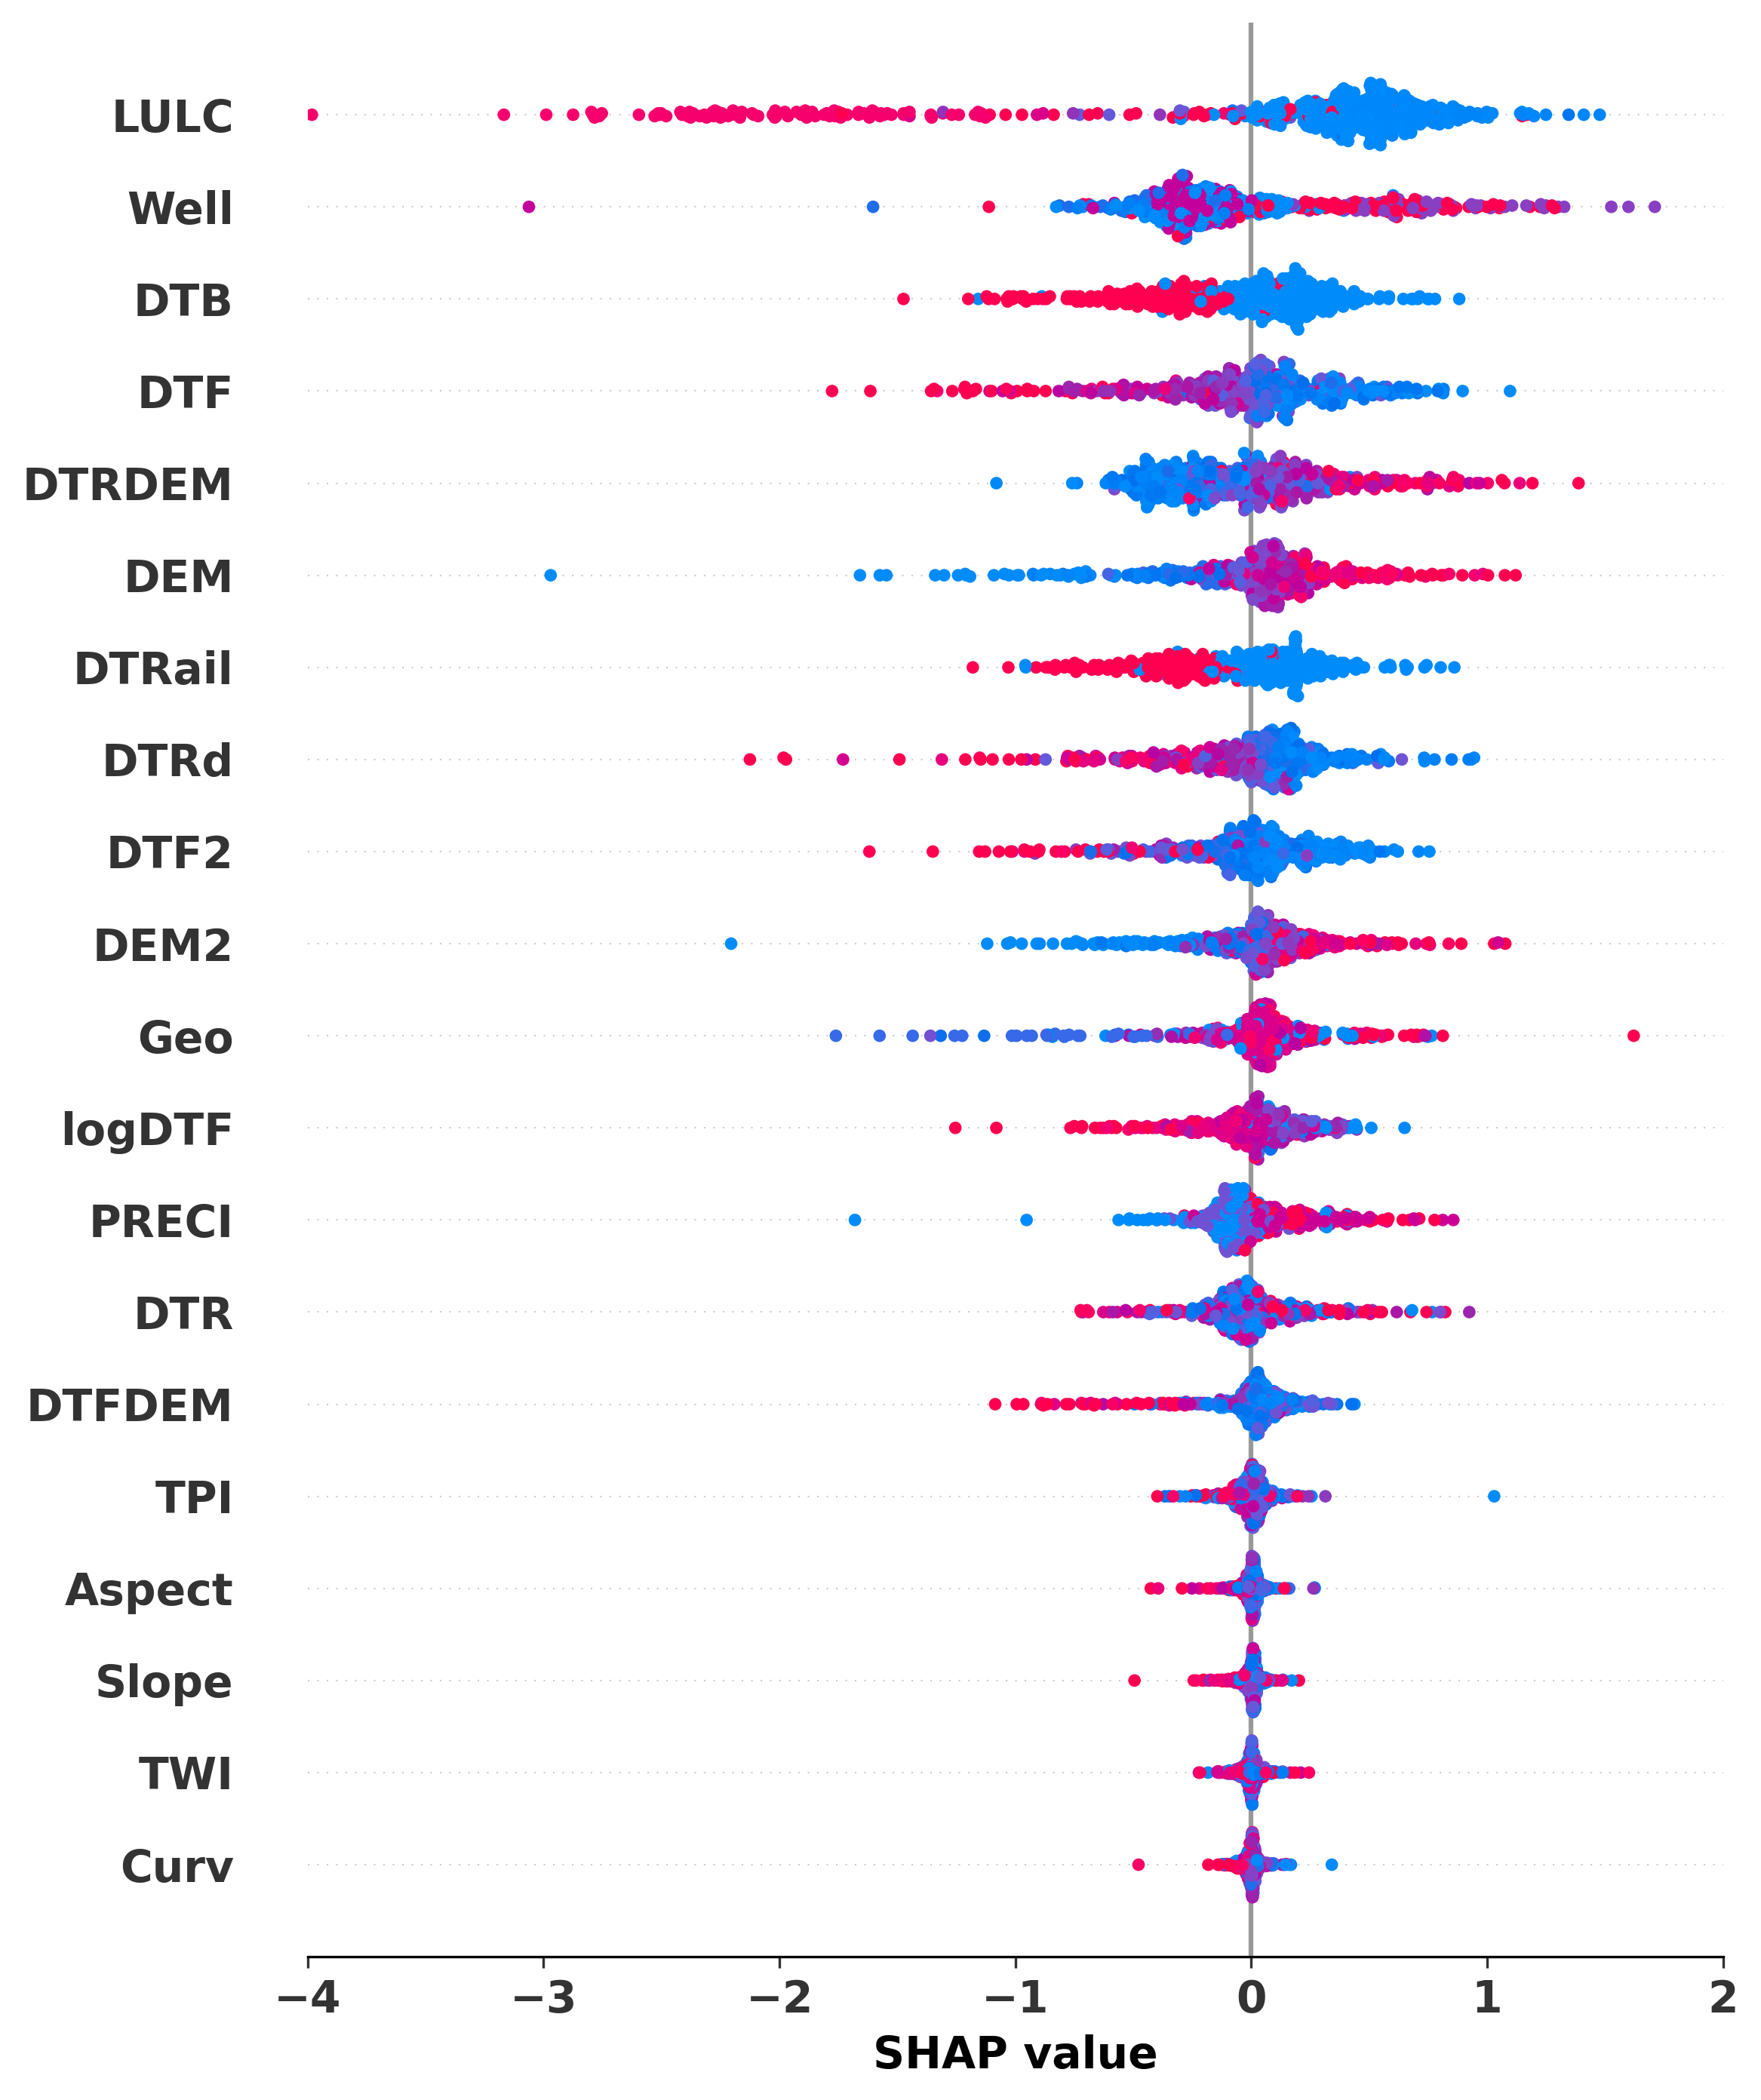
\includegraphics[width=0.48\textwidth]{media/shap_sum_et.png} &
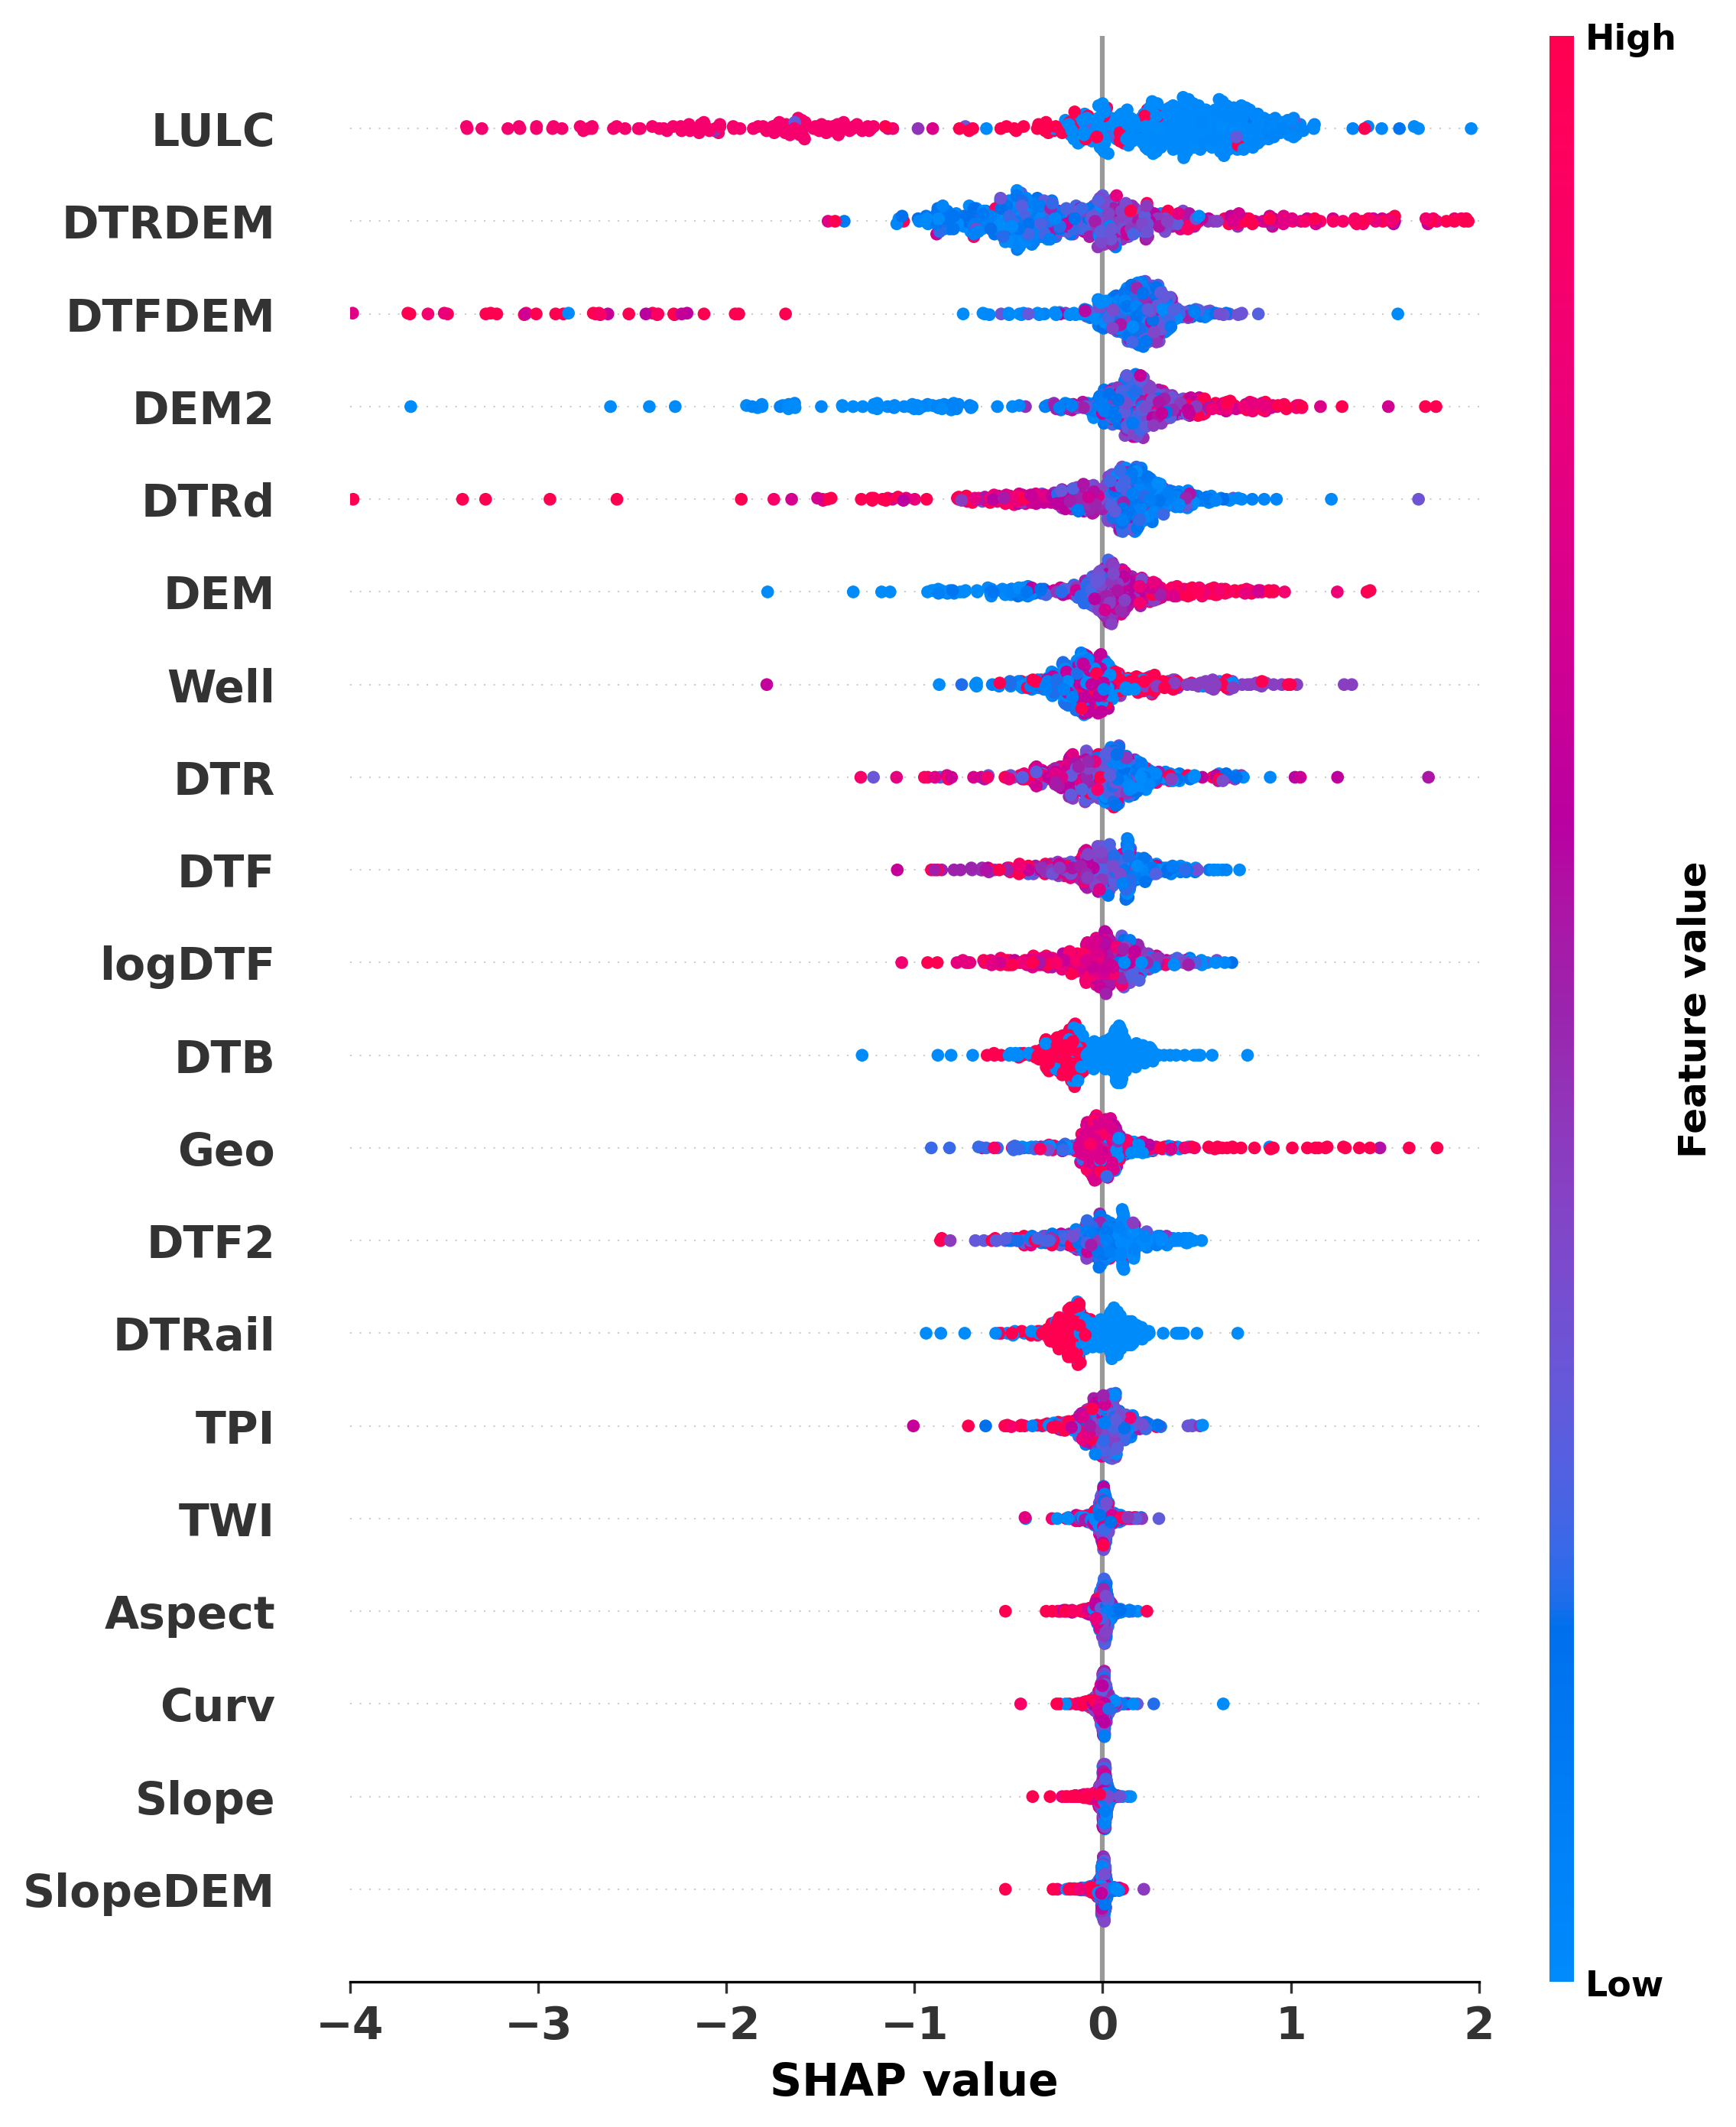
\includegraphics[width=0.48\textwidth]{media/shap_sum_rf.png} \\
(a) SHAP Summary (Extra Trees) & (b) SHAP Summary (Random Forest)
\end{tabular}
\caption{SHAP summary plots: (a) Extra Trees; (b) Random Forest. Color scale: red = high feature value, blue = low.}
\label{fig:shap_summary}
\end{figure}

\begin{figure}[!t]
\centering
\begin{tabular}{cc}
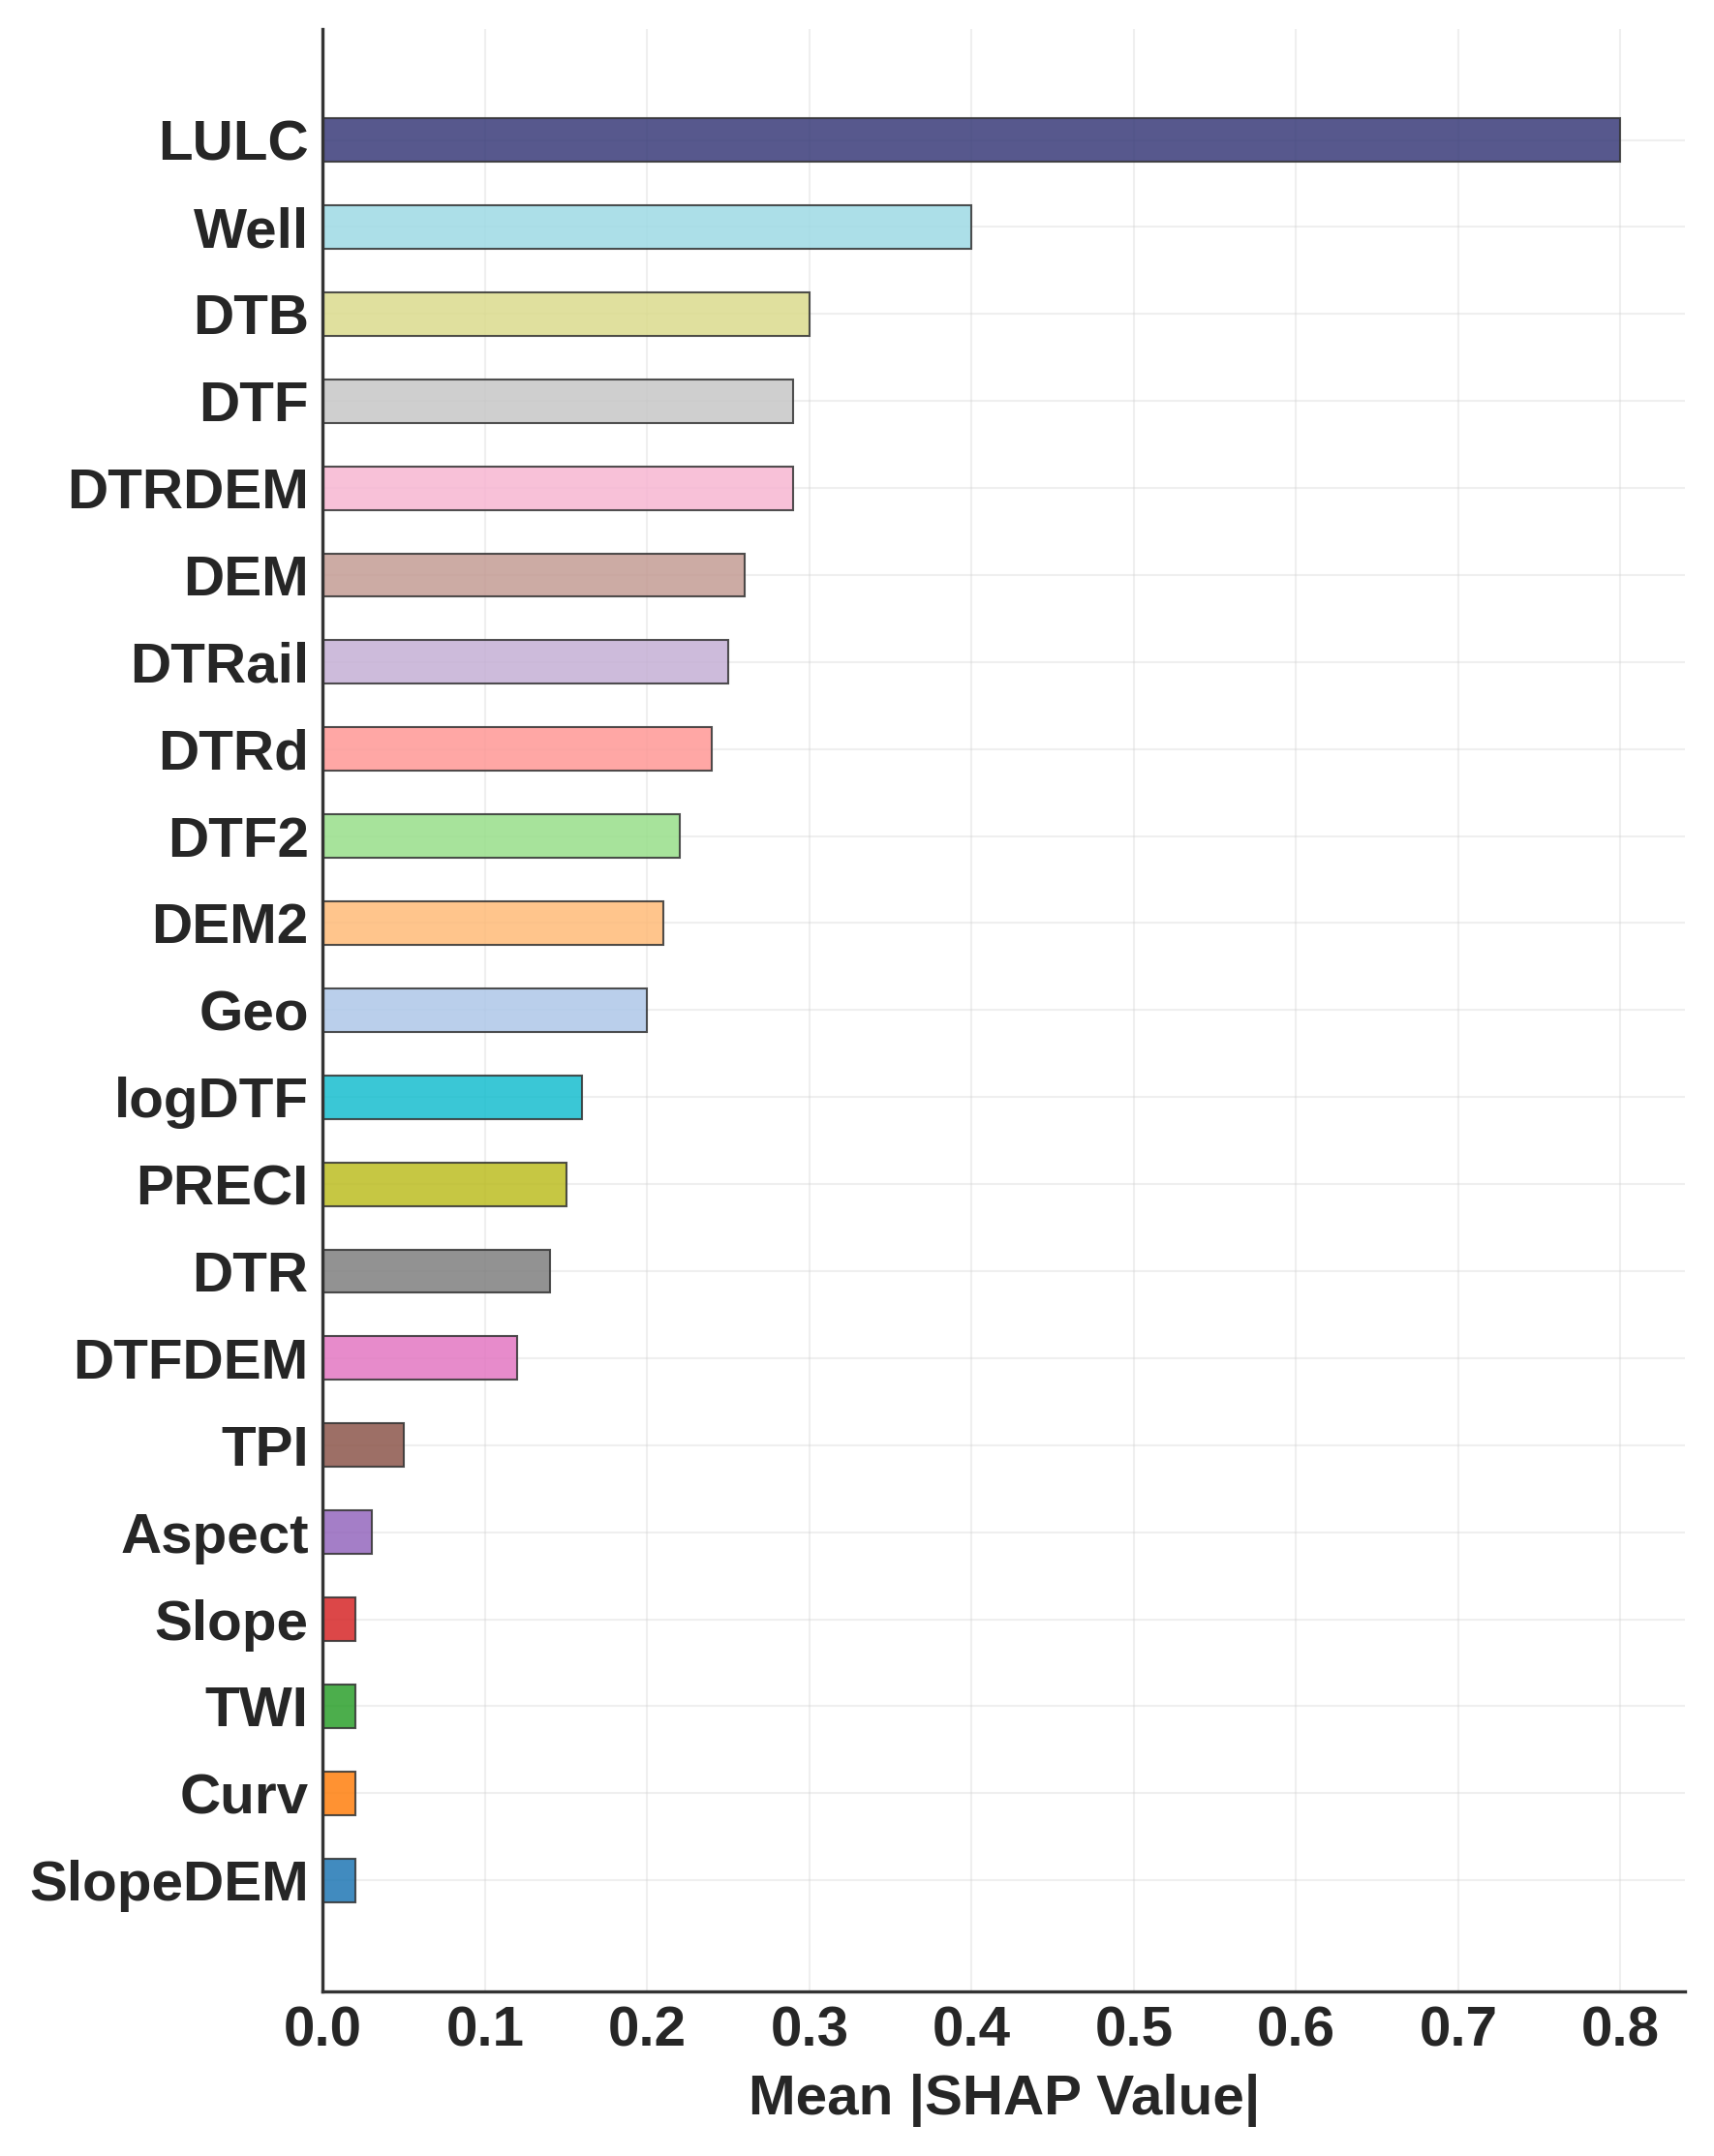
\includegraphics[width=0.48\textwidth]{media/shap_bar_et_slim.png} &
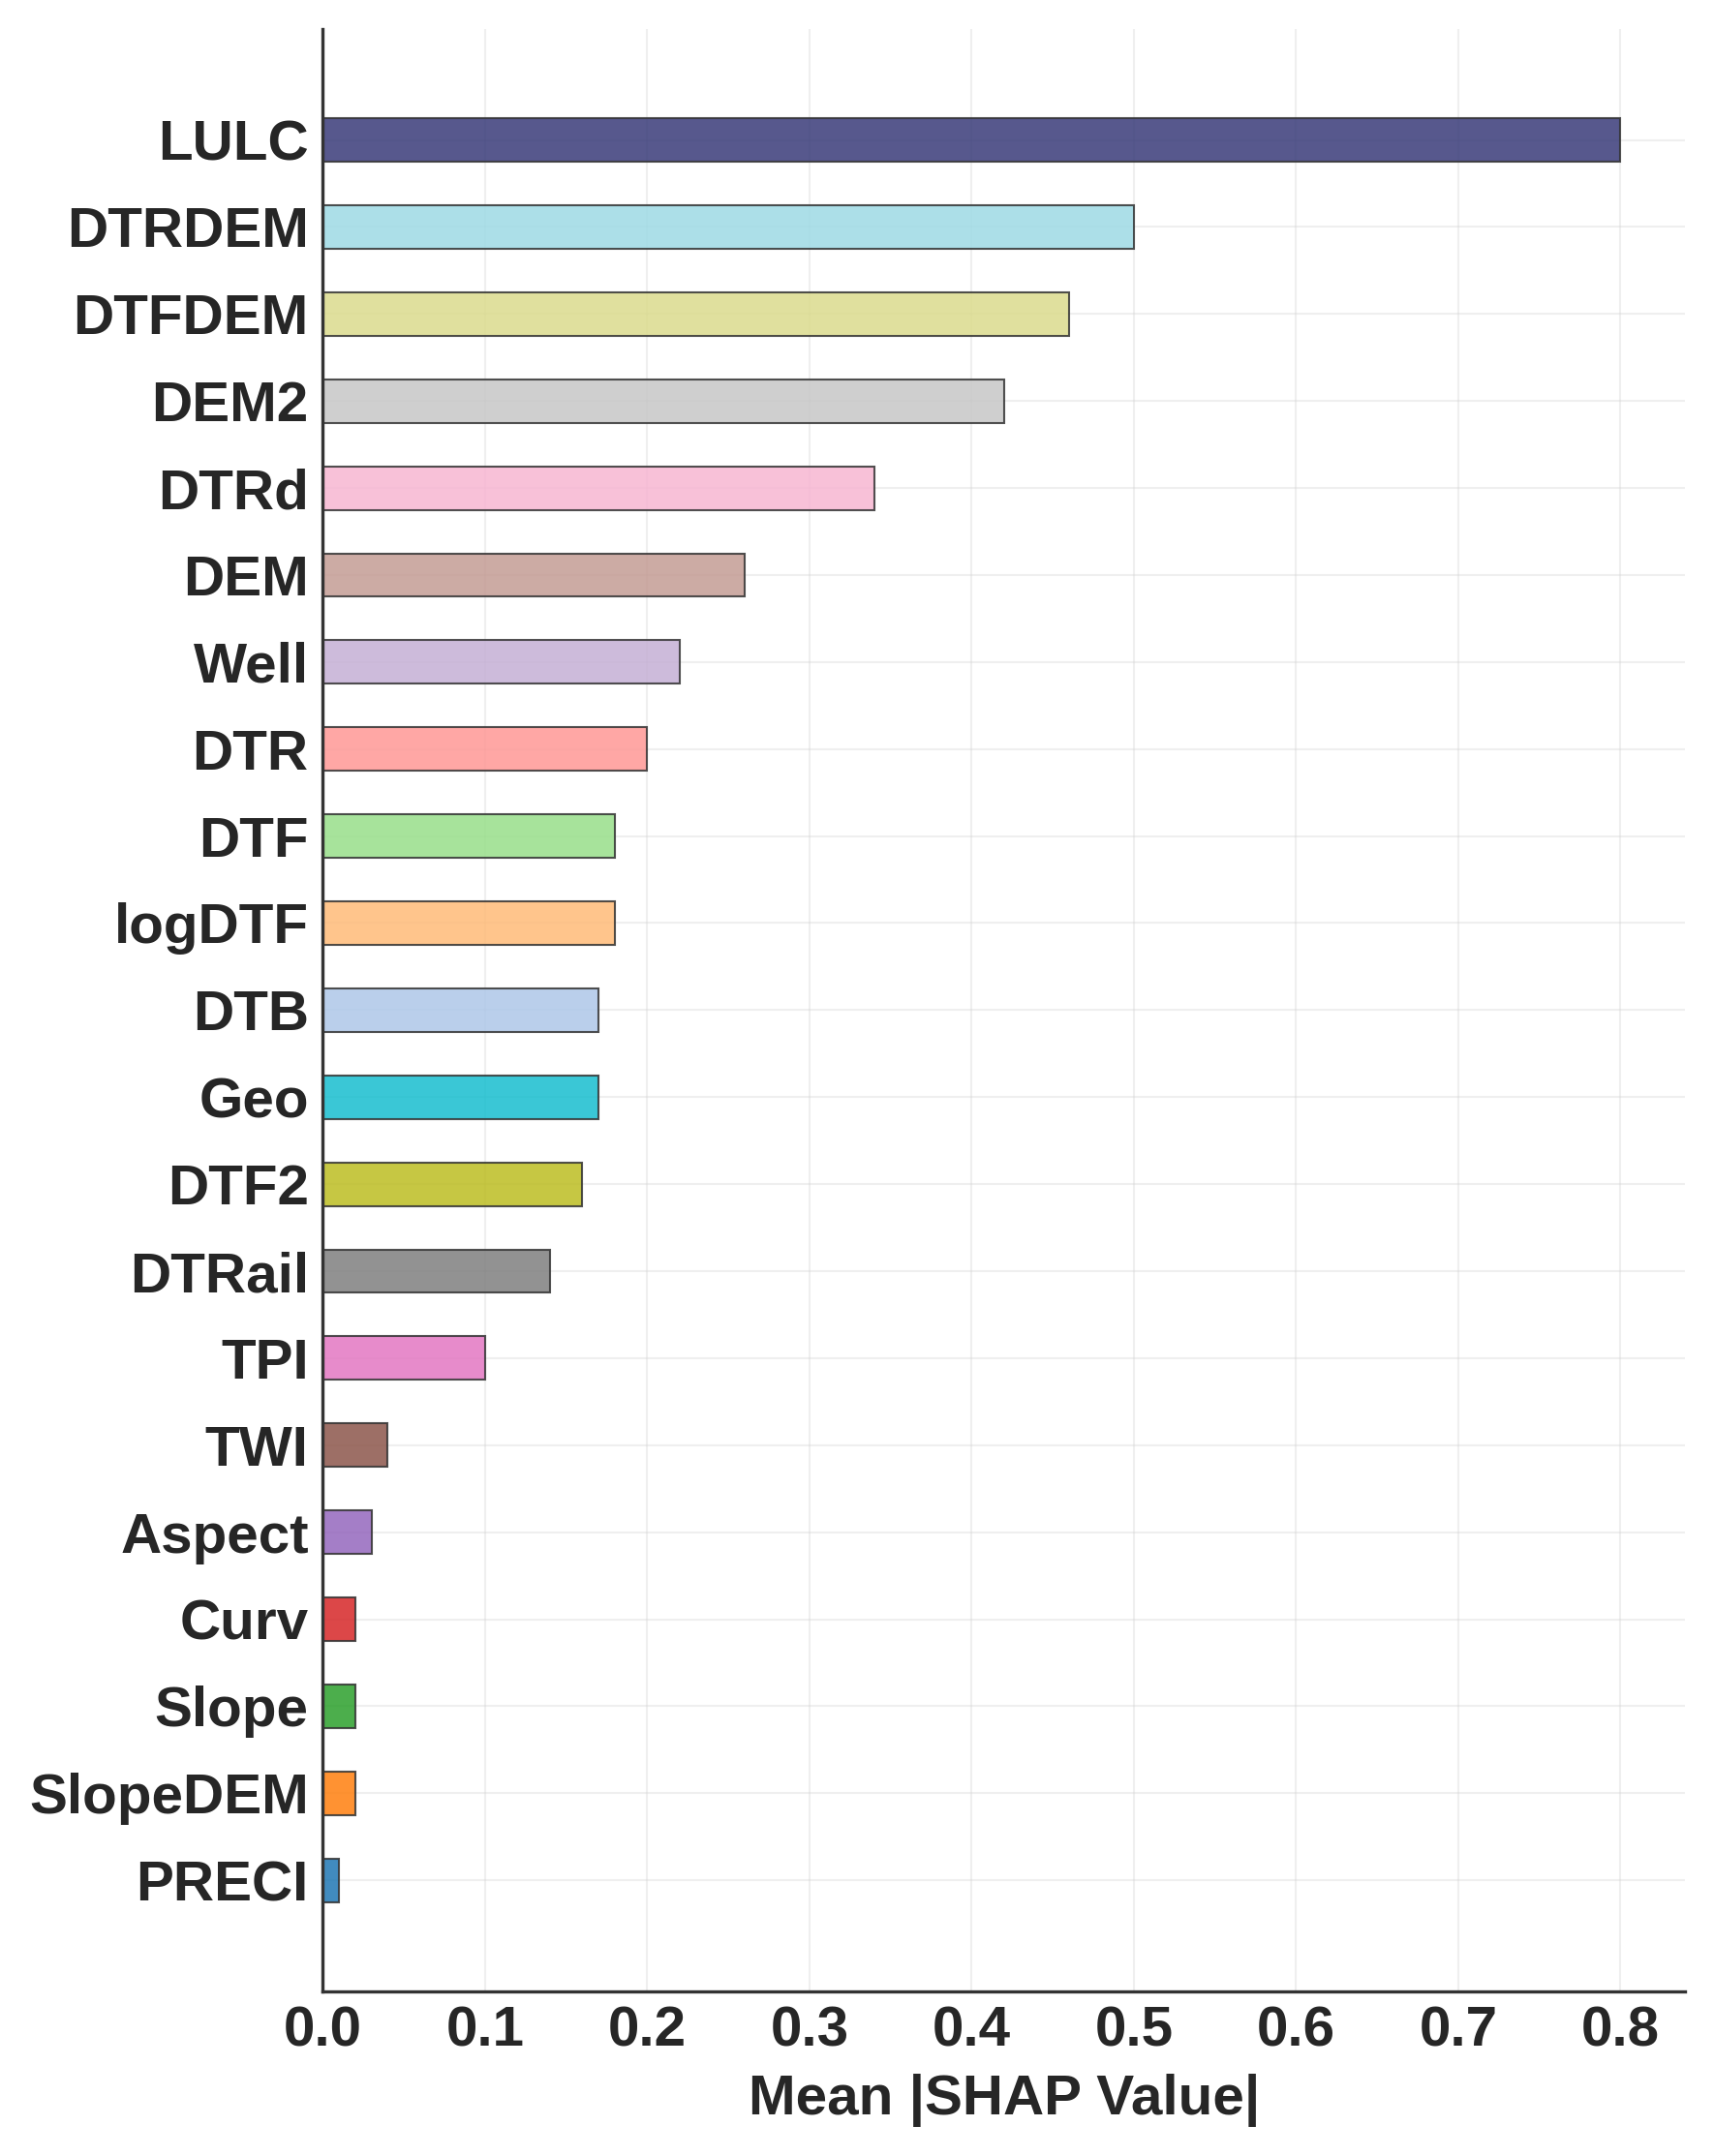
\includegraphics[width=0.48\textwidth]{media/shap_bar_rf_slim.png} \\
(a) SHAP Bar Plot (Extra Trees) & (b) SHAP Bar Plot (Random Forest)
\end{tabular}
\caption{SHAP bar plots showing mean absolute SHAP values: (a) Extra Trees; (b) Random Forest.}
\label{fig:shap_bar}
\end{figure}

LIME analysis (Figures~\ref{fig:lime_et} and \ref{fig:lime_rf}) provides interpretable local explanations for individual predictions. For Extra Trees (Figure~\ref{fig:lime_et}), top positive contributors include LULC, distance from railway, and River\_DEM interaction. For Random Forest (Figure~\ref{fig:lime_rf}), LULC, distance from river, and distance from railway are the dominant contributors. Both models consistently identify LULC as the strongest predictor, confirming that land use is a primary driver of subsidence predictions.

\begin{figure}[!t]
\centering
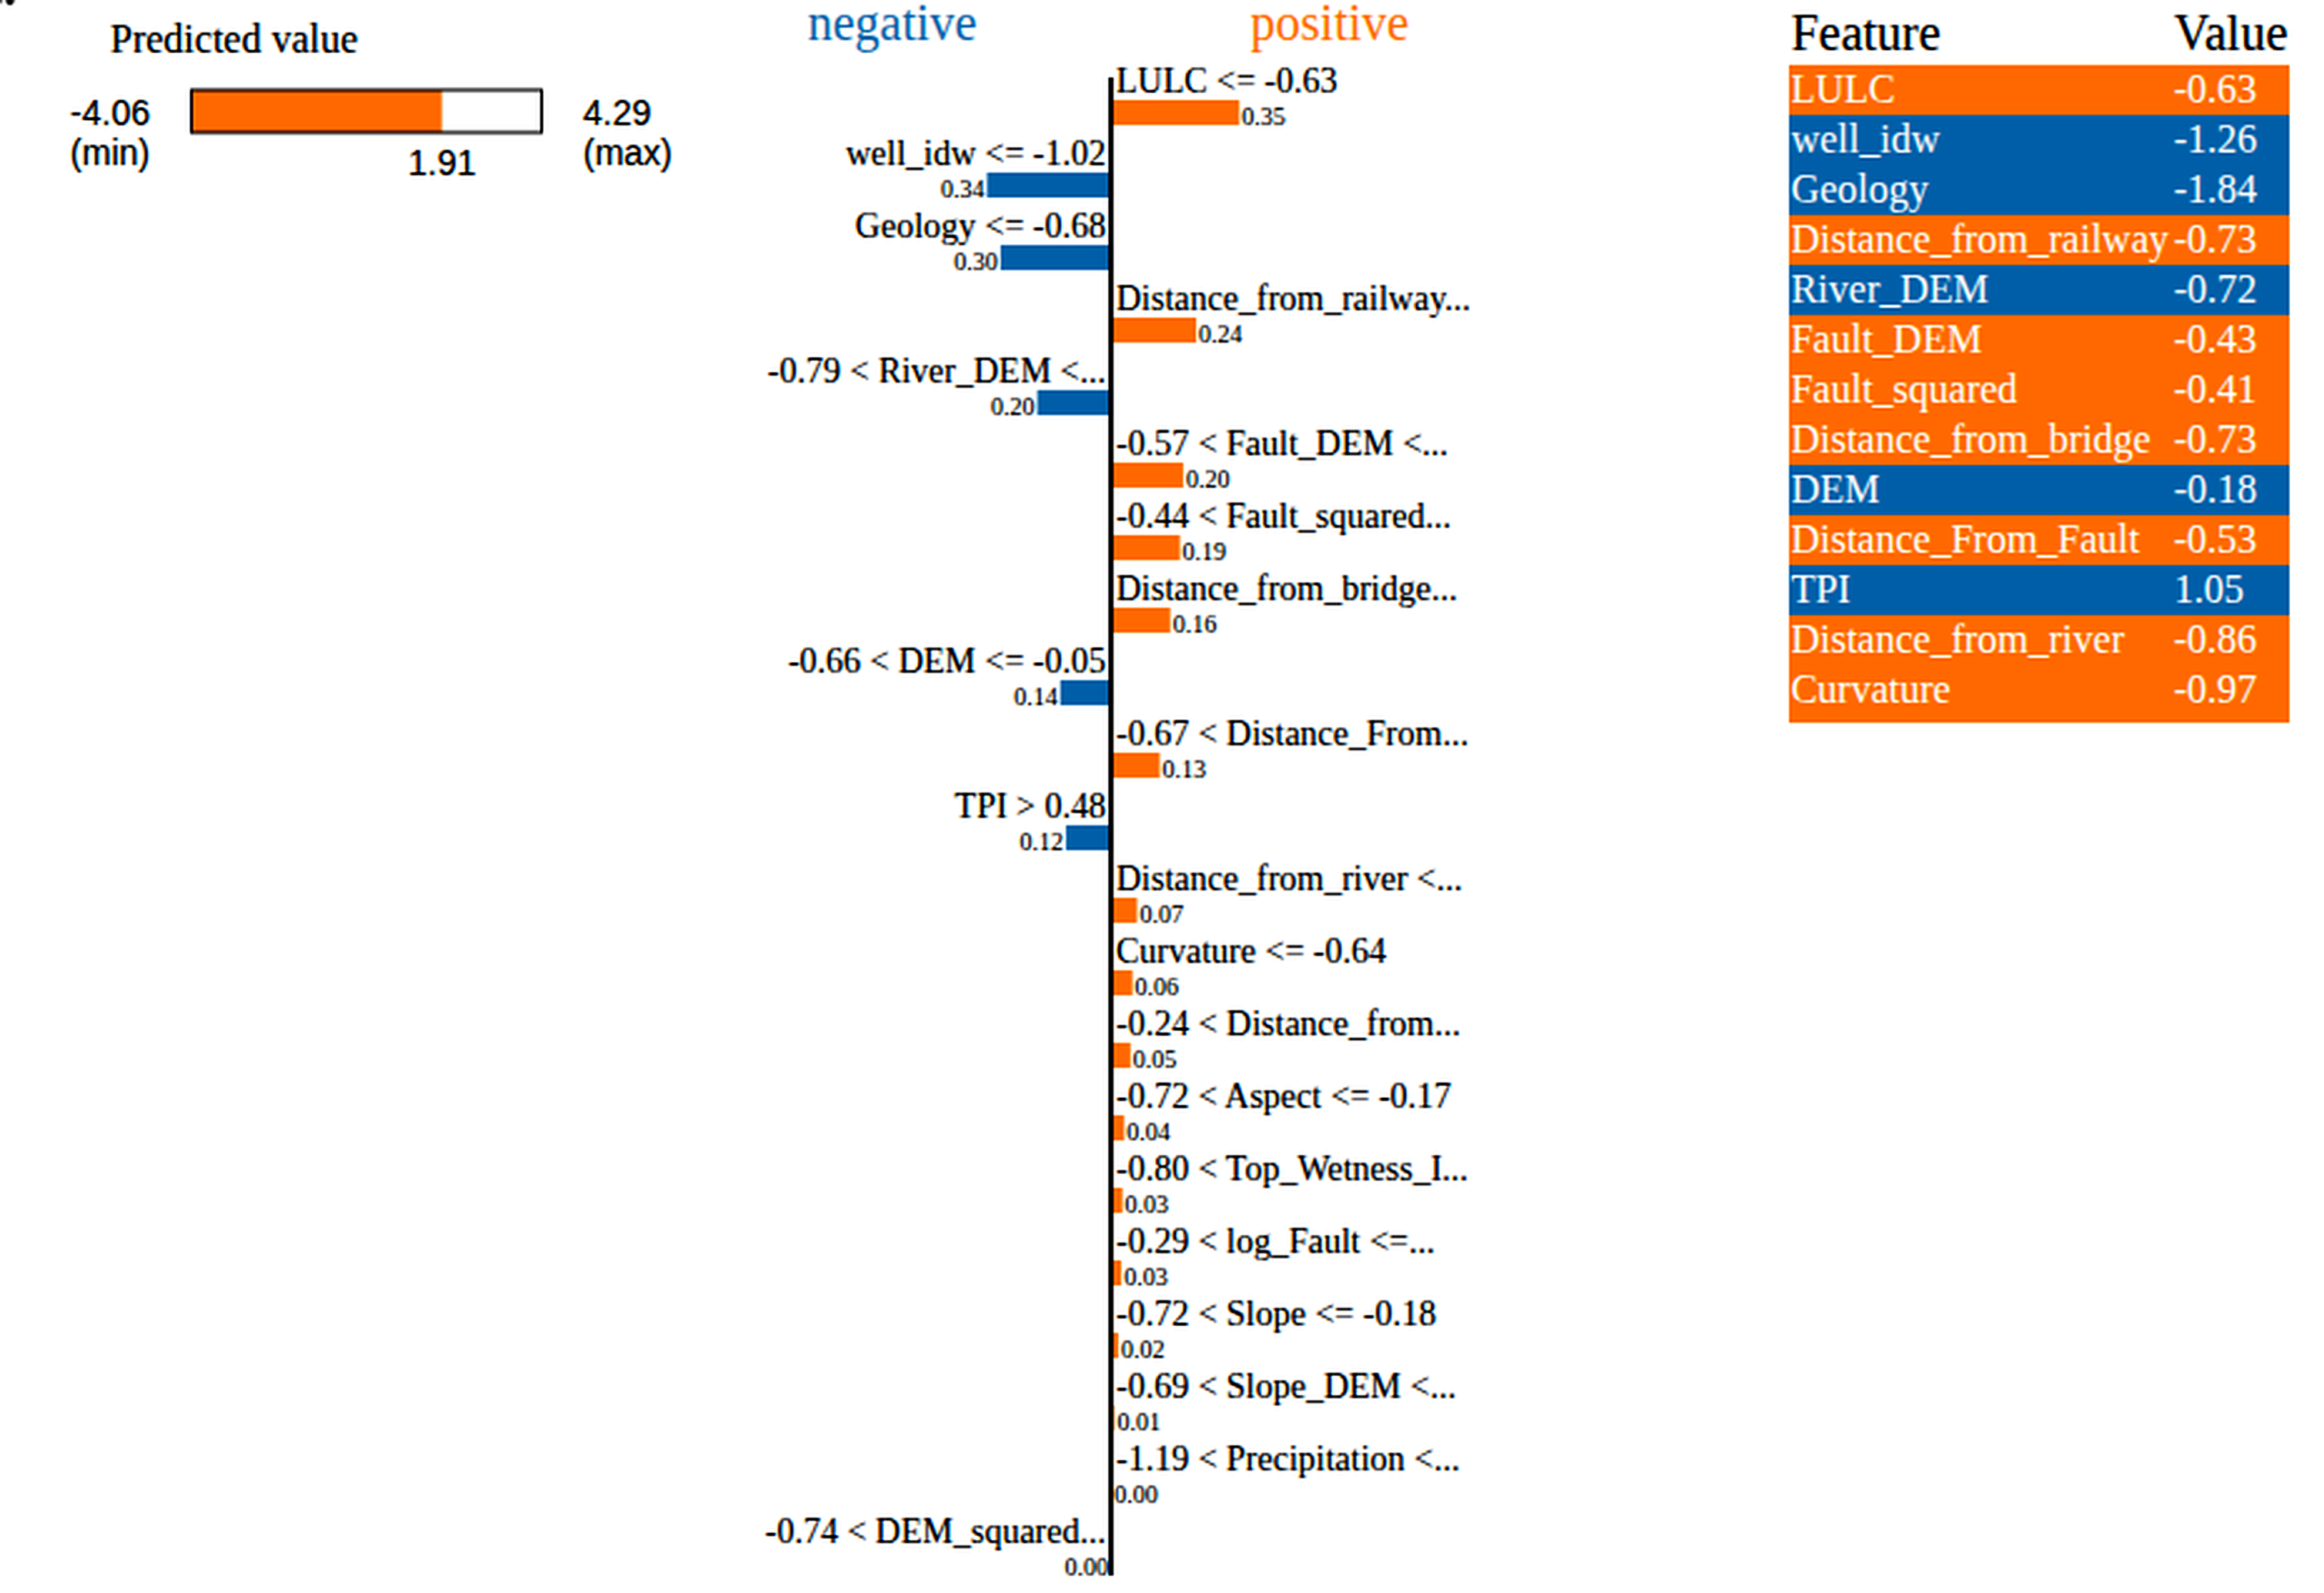
\includegraphics[width=0.85\textwidth]{media/lime_et.png}
\caption{LIME local explanation for Extra Trees model at a representative high-subsidence location. Orange bars indicate positive contributions to subsidence; blue bars indicate negative contributions.}
\label{fig:lime_et}
\end{figure}

\begin{figure}[!t]
\centering
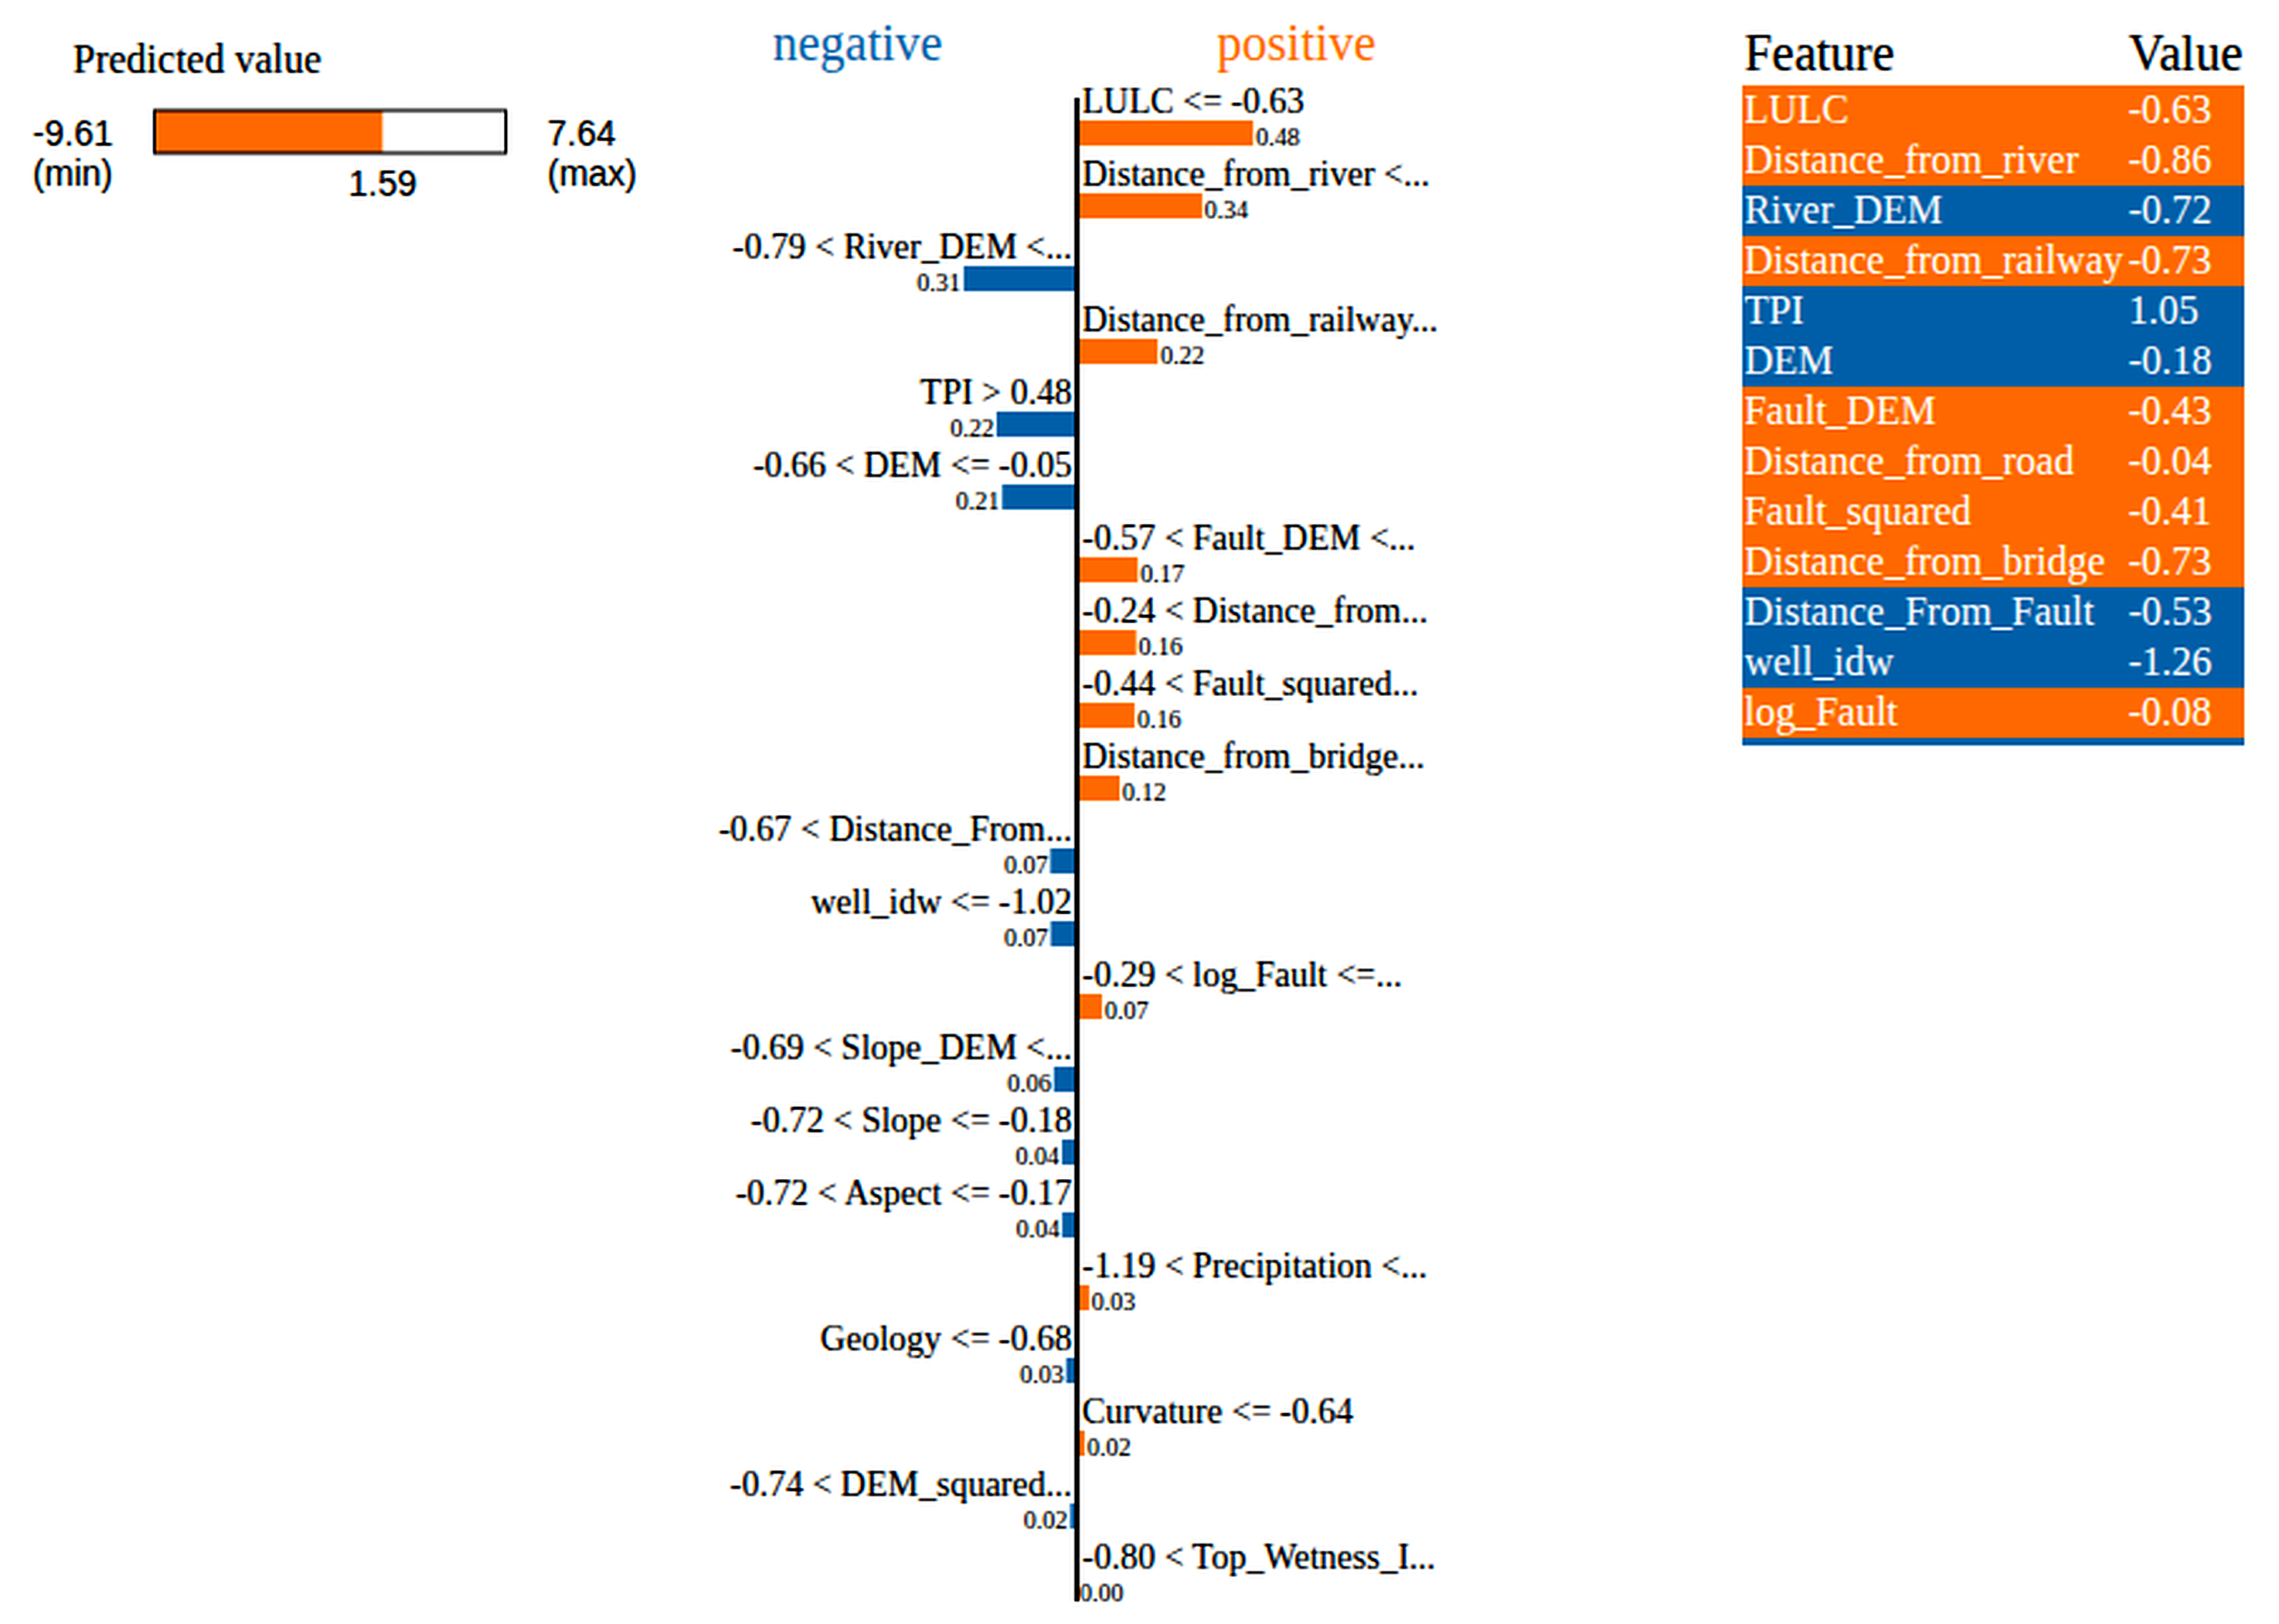
\includegraphics[width=0.85\textwidth]{media/lime_rf.png}
\caption{LIME local explanation for Random Forest model at a representative high-subsidence location. Orange bars indicate positive contributions to subsidence; blue bars indicate negative contributions.}
\label{fig:lime_rf}
\end{figure}

The consistency across MDI, SHAP, and LIME rankings validates the robustness of identified drivers and strengthens confidence in the physical interpretation. LULC, fault proximity, elevation, and groundwater extraction emerge as the dominant factors controlling subsidence in EBRP.


\section{Temporal Forecasting with Physics-Informed LSTM}

The physics-informed Bi-LSTM addresses this limitation by learning sequential deformation dynamics while enforcing geomechanically consistent constraints during long-term extrapolation.

The Bi-LSTM network was trained on 12,847 time-series pixels exhibiting mean velocity $|v| \geq 1.5$~mm/yr, using an 18-month input window and 6-month output horizon. Training on historical data (2017--2023) achieved convergence after 85 epochs. Validation on the held-out period (2024--2025) demonstrates strong performance (Table~\ref{tab:lstm_performance}): $R^2 = 0.834$, RMSE = 18.71~mm, Pearson correlation $r = 0.918$, and Nash-Sutcliffe Efficiency NSE = 0.834.

The strong Pearson correlation ($r = 0.918$) indicates excellent linear correspondence between predicted and observed values, while $R^2 = 0.834$ confirms the model explains 83.4\% of variance in subsidence rates. The physics-informed constraints successfully prevent unphysical trends (velocity reversals, unrealistic acceleration) while maintaining predictive accuracy, demonstrating the value of integrating geomechanical principles with data-driven learning \citep{Zhu2024}.

\begin{table}[!t]
\centering
\caption{Physics-informed LSTM accuracy metrics for the Temporal Forecasting}
\label{tab:lstm_performance}
\begin{tabular}{lc}
\hline
\textbf{Metric} & \textbf{Value} \\
\hline
$R^2$           & 0.834 \\
RMSE (mm)       & 18.71 \\
MAE (mm)        & 14.26 \\
Pearson $r$     & 0.918 \\
NSE             & 0.834 \\
Bias (mm)       & $-4.03$ \\
\hline
\end{tabular}
\end{table}

Autoregressive forecasting to 2030 (Figure~\ref{fig:lstm_forecast_results}) predicts continuous subsidence with a mean velocity of $-0.530$~mm/yr by 2030. 
The forecasted velocity map (Figure~\ref{fig:lstm_forecast_results}a) shows subsidence ranging from $-19.54$ to $-3.36$~mm/yr concentrated in the southern parish, with uplift ($1.31$ to $8.65$~mm/yr) in the northern regions. The susceptibility classification (Figure~\ref{fig:lstm_forecast_results}b) maintains the same five risk levels, with Very High risk zones persisting in the southern urban corridor.

\begin{figure}[!t]
\centering
\begin{tabular}{cc}
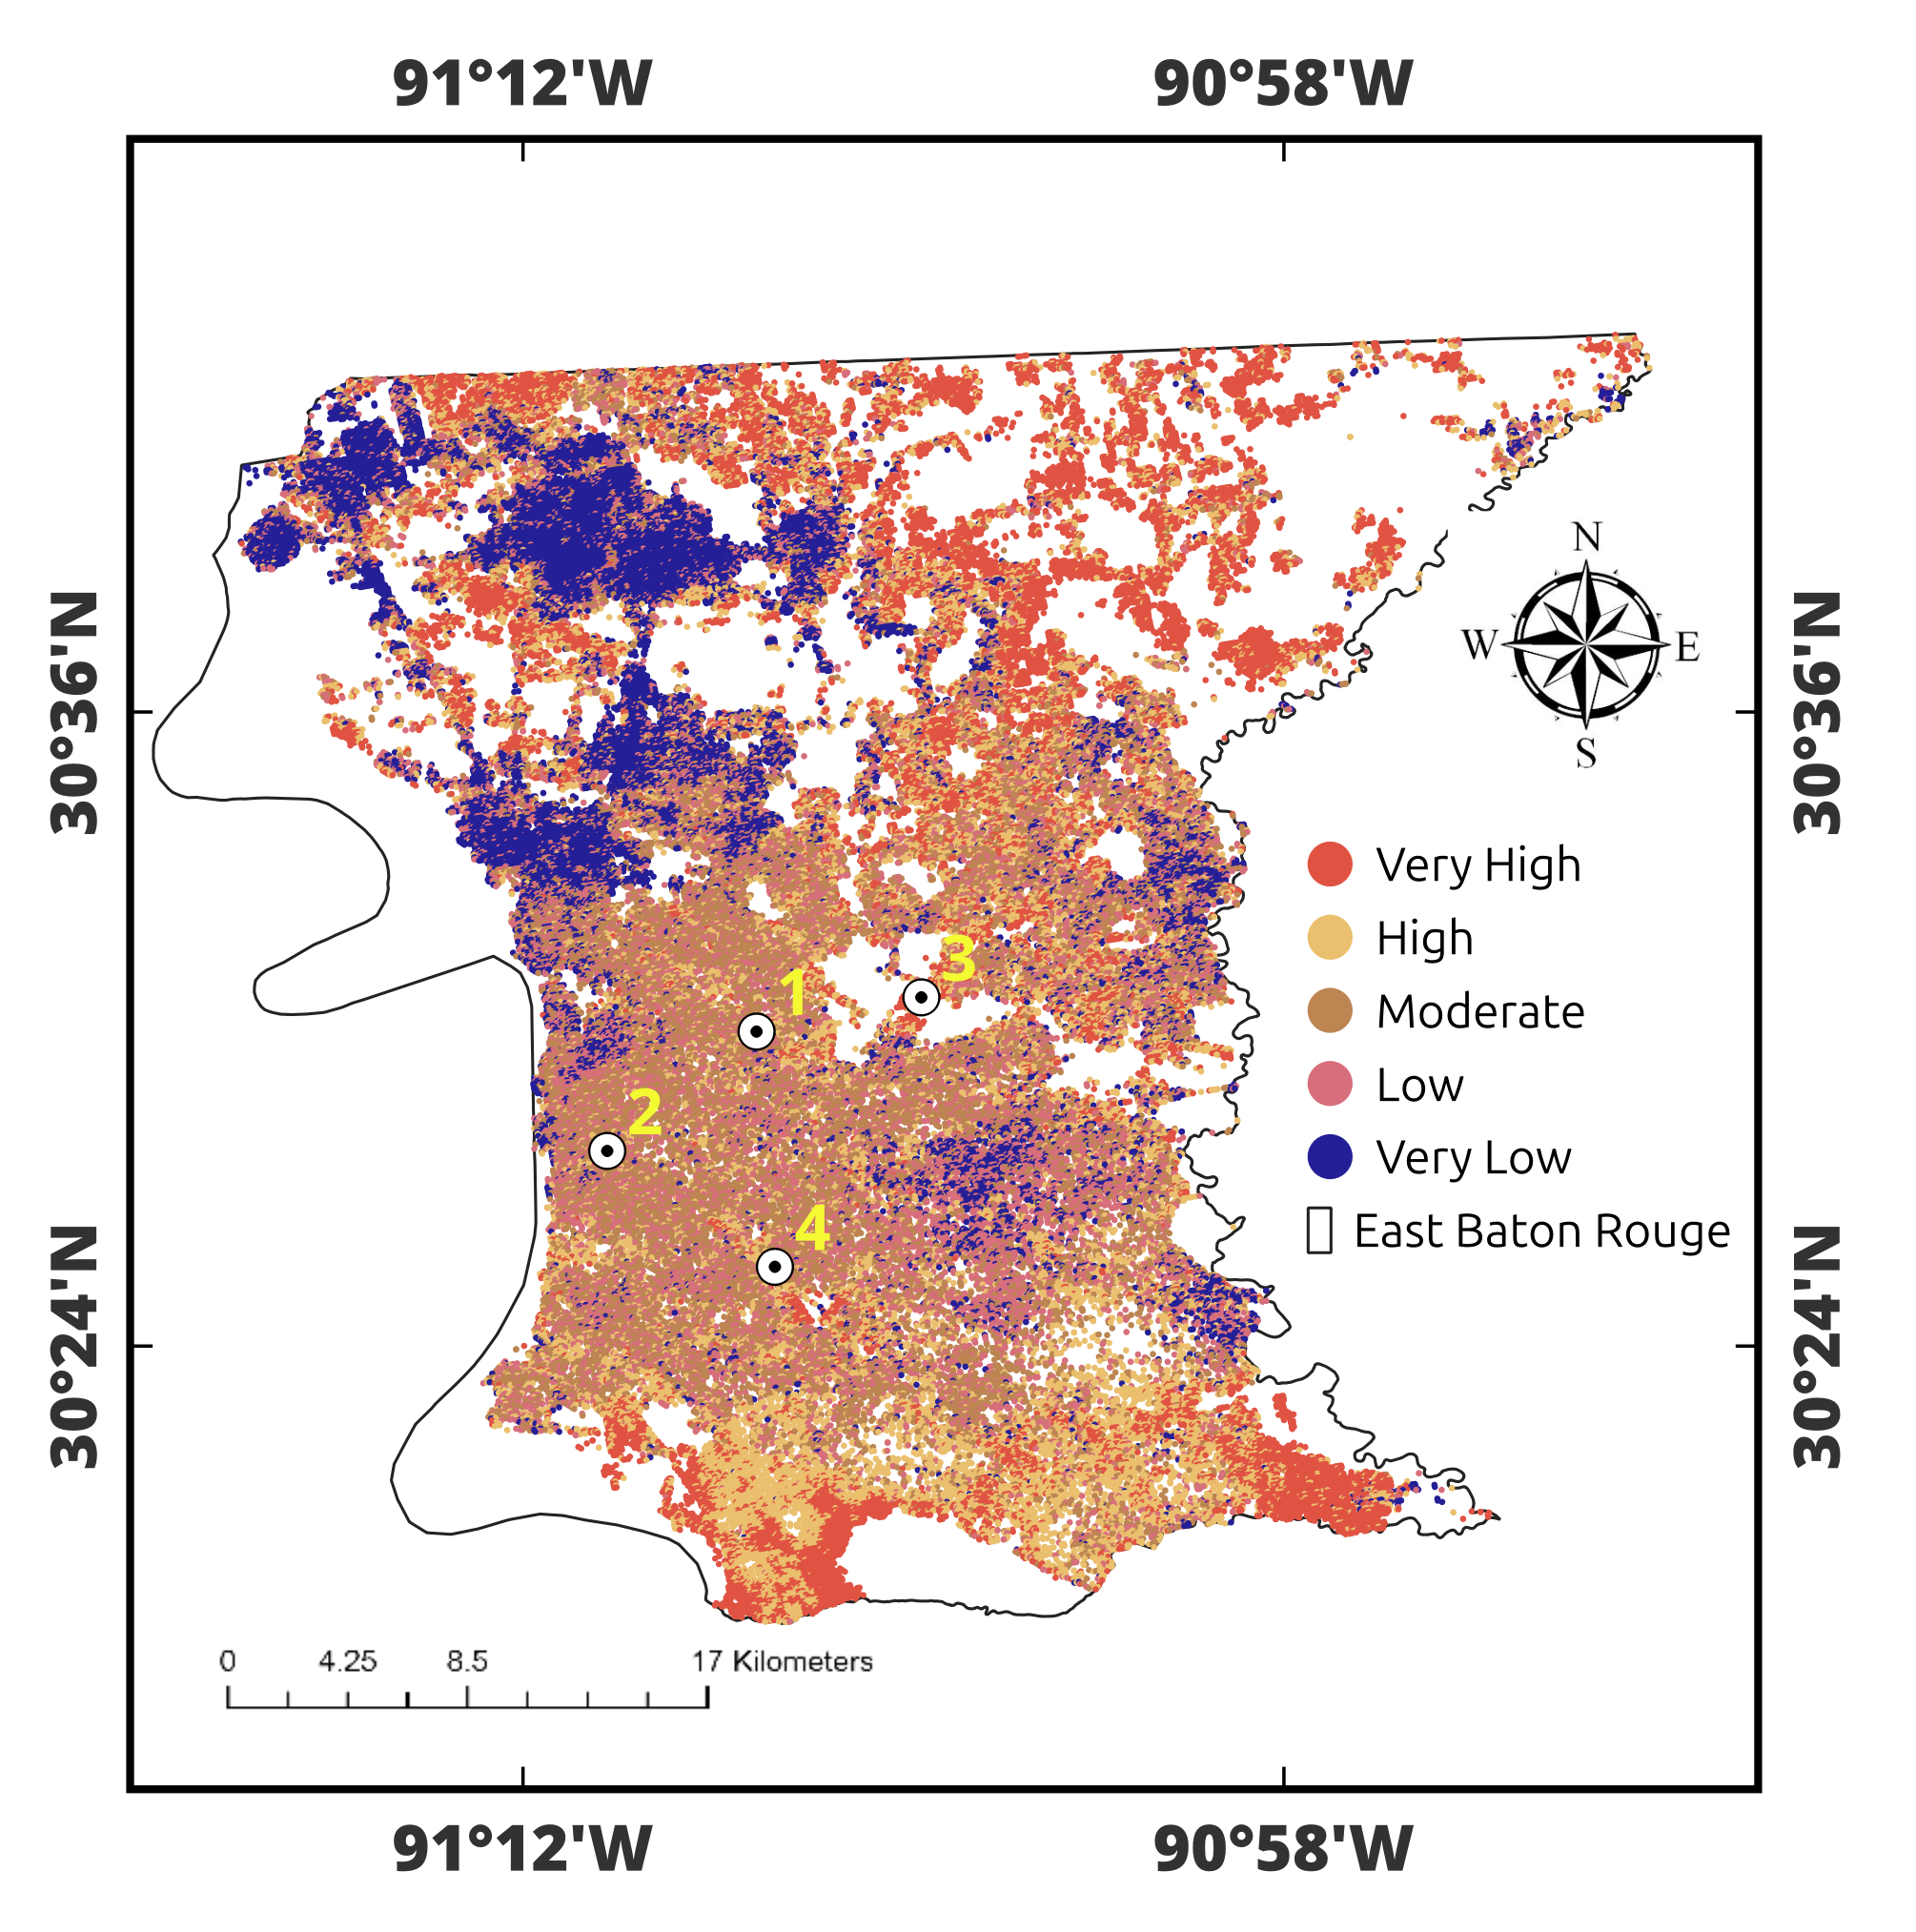
\includegraphics[width=0.48\textwidth]{media/lstm_vel2.png} &
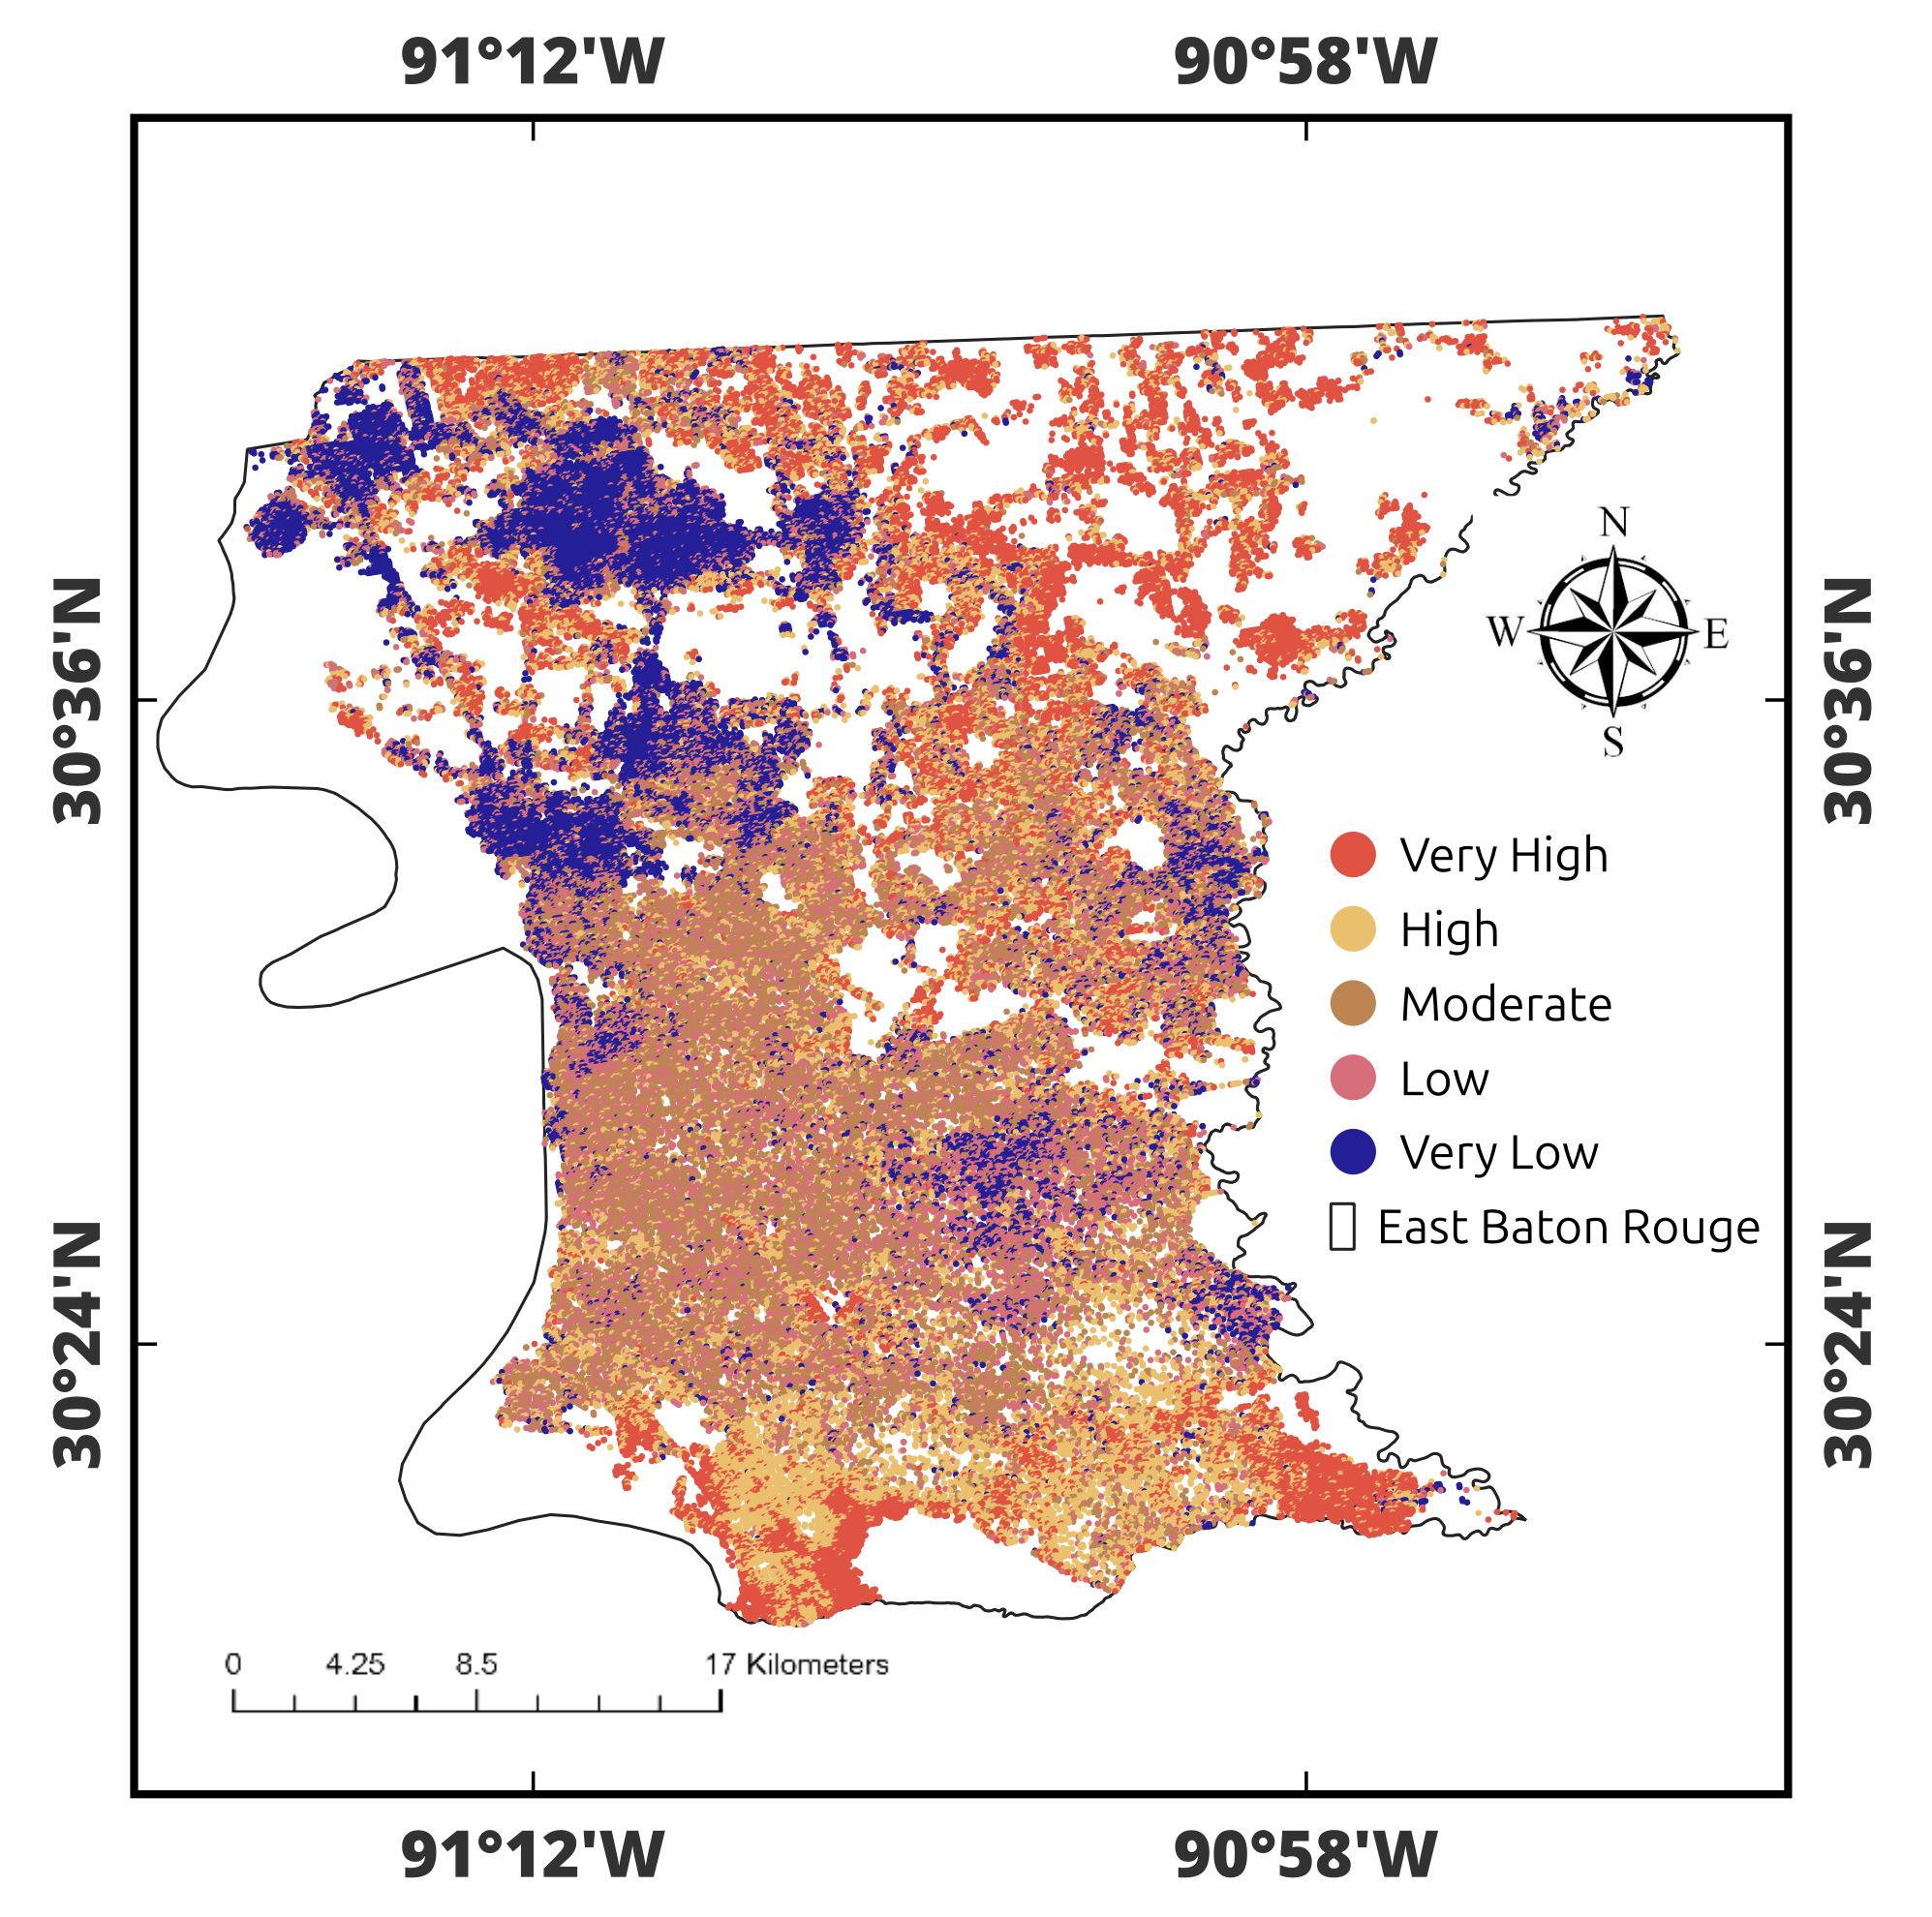
\includegraphics[width=0.48\textwidth]{media/lstm_susc2.png} \\
(a) LSTM Forecasted Velocity & (b) LSTM Forecasted Susceptibility
\end{tabular}
\caption{Physics-informed LSTM forecasts to 2030: (a) Predicted velocity showing continued subsidence; (b) Forecasted susceptibility classification indicating persistent high-risk zones.}
\label{fig:lstm_forecast_results}
\end{figure}

Time-series forecasts at four representative locations (Figure~\ref{fig:lstm_timeseries}) reveal spatially heterogeneous 
subsidence behavior controlled by geological and land-use characteristics. Location 1 (Winbourne/Foster area) sits on Pleistocene Prairie Terraces with relatively stable, stiffer clay-rich soils, exhibiting a subsidence trend of $-8.10$~mm/yr with total displacement of $-197.69$~mm. Location 2 (Downtown, State Capitol/Main St) represents the urbanized core near the Mississippi River levee and active fault traces, showing the lowest subsidence rate ($-5.02$~mm/yr, total $-122.57$~mm). Location 3 (Merrydale, Greenwell Springs/Airline) lies within the active fault zone between the Baton Rouge and Denham Springs faults, with moderate subsidence ($-6.72$~mm/yr, total $-164.03$~mm). Location 4 (LSU Lakes, Stanford Ave area) consists of Holocene-age sediments that are highly prone to compaction, exhibiting the highest subsidence rate ($-12.25$~mm/yr, total $-299.12$~mm).

\begin{figure}[!t]
\centering
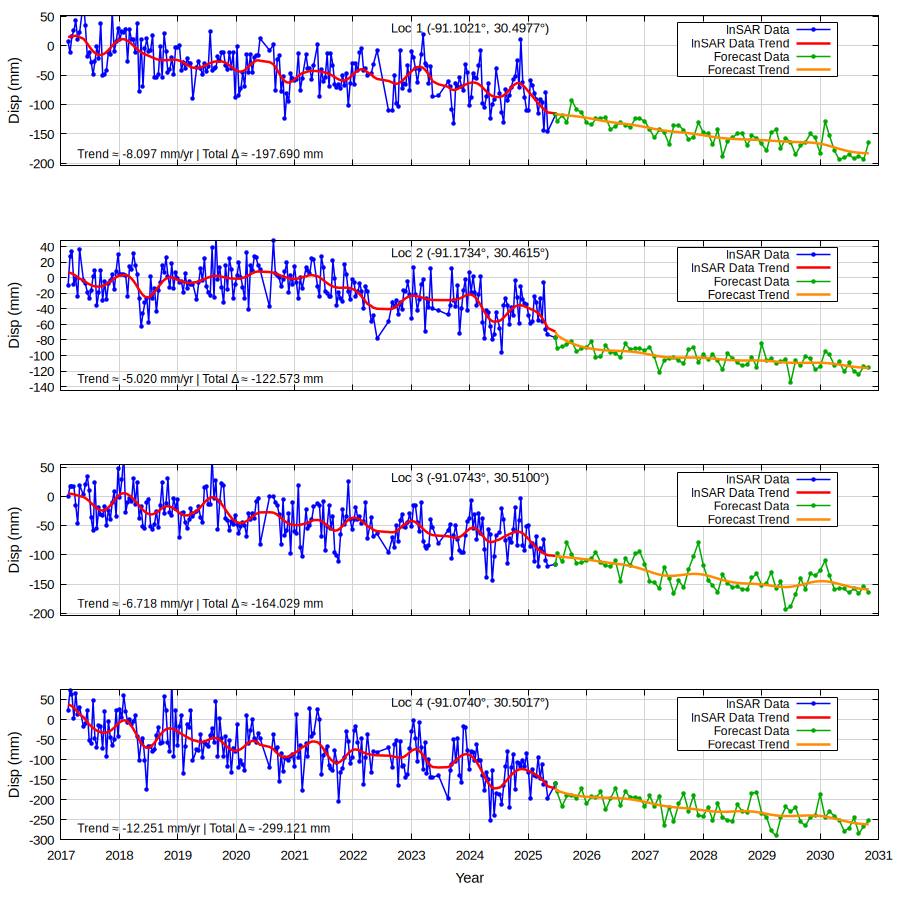
\includegraphics[width=0.95\textwidth]{media/lstm_ts.png}
\caption{Forecasted time-series at four representative locations (1--4) showing varied subsidence patterns. Blue: InSAR observations (2017--2025); green/orange: LSTM forecasts (2025--2030). Smooth transitions demonstrate physics-constraint effectiveness.}
\label{fig:lstm_timeseries}
\end{figure}

The physics-informed constraints effectively reduce forecast uncertainty, with one-year-ahead forecasts showing $\pm 2.1$~mm/yr uncertainty growing to $\pm 4.8$~mm/yr for five-year forecasts. The cumulative displacement results highlight areas requiring continued monitoring, particularly zones with high subsidence rates where critical infrastructure may be affected.


\section{Integrated Assessment and Implications}

The spatial susceptibility mapping (ET) and temporal forecasting (physics-informed LSTM) provide separate but complementary perspectives on subsidence risk. Time-series analysis at four representative locations demonstrates how geological setting controls subsidence behavior: LSU Lakes ($-12.25$~mm/yr) on compressible Holocene sediments shows the highest rates, while Downtown ($-5.02$~mm/yr) near the Mississippi River levee exhibits the lowest. North Baton Rouge ($-8.10$~mm/yr) on stable Pleistocene terraces and Merrydale ($-6.72$~mm/yr) within the active fault zone show intermediate rates. These findings confirm that both sediment age/compressibility and proximity to geological structures control subsidence magnitude.

The results provide actionable information for stakeholders: restricting high-density development within 2~km of fault systems, assessing critical infrastructure in zones exceeding $-10$~mm displacement by 2030, regulating groundwater extraction in high-well-density clusters, integrating subsidence risk into flood modeling and levee maintenance, and expanding InSAR monitoring and GNSS coverage in fault-proximal areas.


\chapter[Conclusions and Recommendations]{\centering Conclusions and Recommendations}

\section{Conclusions}

This study established an integrated framework to map and forecast land subsidence in East Baton Rouge Parish using SBAS-InSAR and machine learning. Ground deformation from 2017–2025 showed spatial variability, with subsidence concentrated in southern urban areas near faults and uplift in the north. The Extra Trees model predicted deformation more accurately than Random Forest and closely matched InSAR observations, while feature analysis identified land use/land cover, proximity to faults, elevation, and drainage distance as the main drivers. A physics-informed Bi-LSTM projected continued subsidence through 2030, with higher rates near the Mississippi River and LSU Lakes, and moderate rates in North Baton Rouge and Merrydale. Overall, geological conditions—especially compressible Holocene sediments and proximity to active faults—are the dominant controls on subsidence magnitude.


\section{Recommendations}

Based on the findings, the following recommendations are provided: restricting high-density development within 2~km of fault systems and incorporating subsidence risk into zoning regulations; conducting structural assessments for critical infrastructure in zones with high subsidence rates, particularly areas exceeding $-10$~mm/yr; regulating groundwater extraction in high-well-density clusters; and expanding GNSS coverage and integrating multi-satellite InSAR for improved monitoring.

\clearpage
\phantomsection
\addcontentsline{toc}{chapter}{References}
\printbibliography[title={References}]

\end{document}
